\chapter{System Design}
\label{ch:system_design}

\section{Introduction to System Design}
Designing an institutional-grade, fiduciary portfolio management platform for retail investors in the Indian equity market requires addressing dual, conflicting technical challenges: ensuring high conversational intelligence and explainability through modern Artificial Intelligence (AI) models, while strictly guaranteeing arithmetic correctness, regulatory compliance, and exchange execution feasibility.

To achieve this, \textbf{Lucid} adheres to a fundamental architectural design philosophy: \textit{the complete decoupling of qualitative multi-agent reasoning from deterministic quantitative optimization and stateful persistence}. Rather than relying on Large Language Models to compute portfolio percentages or generate trade orders---which risks mathematical hallucinations, non-normalizing weights, and non-tradable fractional shares---Lucid confines AI agents to qualitative synthesis, corporate governance scrutiny, and retail-accessible explanation generation. All numerical weights, risk constraints, integer share counts, and fee calculations are executed strictly by deterministic mathematical algorithms.

This chapter unifies the complete engineering blueprint of Lucid across seven interconnected architectural dimensions:
\begin{enumerate}
    \item \textbf{System Architecture and Runtime Topology} (Section~\ref{sec:system_arch}): The overarching six-tier decoupled architecture, component boundaries, runtime execution loops, technology stack selections, and enterprise security safeguards.
    \item \textbf{High-Level Design (HLD)} (Section~\ref{sec:hld}): The core functional subsystem decomposition, information movement pathways, end-to-end user workflows, and pivotal design decisions.
    \item \textbf{Low-Level Design (LLD)} (Section~\ref{sec:lld}): The internal software mechanics, modular React/Next.js frontend architecture, 13-node LangGraph multi-agent research committee, SciPy SLSQP numerical engine, and market-hours background monitoring daemon.
    \item \textbf{End-to-End Methodology} (Section~\ref{sec:methodology}): The structured multi-stage mathematical and algorithmic pipeline governing portfolio creation, Demat Consolidated Account Statement (CAS) portfolio diagnosis, and market-hours drift monitoring with statutory tax-aware rebalancing.
    \item \textbf{Database Design and Schema Architecture} (Section~\ref{sec:database_design}): The relational persistence foundation housing 62 domain tables, relational integrity constraints, master Entity-Relationship (ER) model, and audit versioning.
    \item \textbf{Datasets Used and External Data Sources} (Section~\ref{sec:dataset}): The complete operational universe covering 2,639 listed NSE/BSE equities, ingestion from Yahoo Finance, FRED macroeconomic indicators, and news sentiment feeds.
    \item \textbf{API Contract and Interface Specifications} (Section~\ref{sec:api_contract}): The RESTful communication interface encompassing 82 production endpoints across 9 routers, OpenAPI schemas, and end-to-end client-server interaction sequence flows.
\end{enumerate}


\section{System Architecture and Runtime Topology}
\label{sec:system_arch}
\label{ch:system_arch}

\subsection{System Architecture Overview}
The system architecture of Lucid describes how all the user interface components, backend API gateways, artificial intelligence agents, mathematical optimization solvers, and relational databases are organized so that the application runs quickly, reliably, and securely.

To guarantee high speed and financial accuracy, Lucid strictly separates qualitative artificial intelligence reasoning from quantitative mathematical optimization. The entire platform is engineered as a \textbf{Six-Tier Decoupled Architecture} organized in an end-to-end processing loop across two balanced functional rows:
\begin{itemize}
    \item \textbf{Top Processing Row (Forward User \& Research Flow)}: Connects the investor from the Next.js client interface (Tier 1) through the FastAPI security gateway (Tier 2) to the LangGraph multi-agent intelligence committee (Tier 3).
    \item \textbf{Bottom Processing Row (Optimization \& Storage)}: Dispatches vetted candidate stocks into the SciPy solver (Tier 4), saves portfolio decisions into PostgreSQL (Tier 5), and pulls live market feeds from Indian exchange archives (Tier 6).
\end{itemize}

Figure~\ref{fig:sys_arch_diagram} illustrates the complete six-tier architectural topology of Lucid, detailing the exact technologies, component boundaries, inputs, and outputs across all subsystems:

\begin{figure}[!htbp]
    \centering
    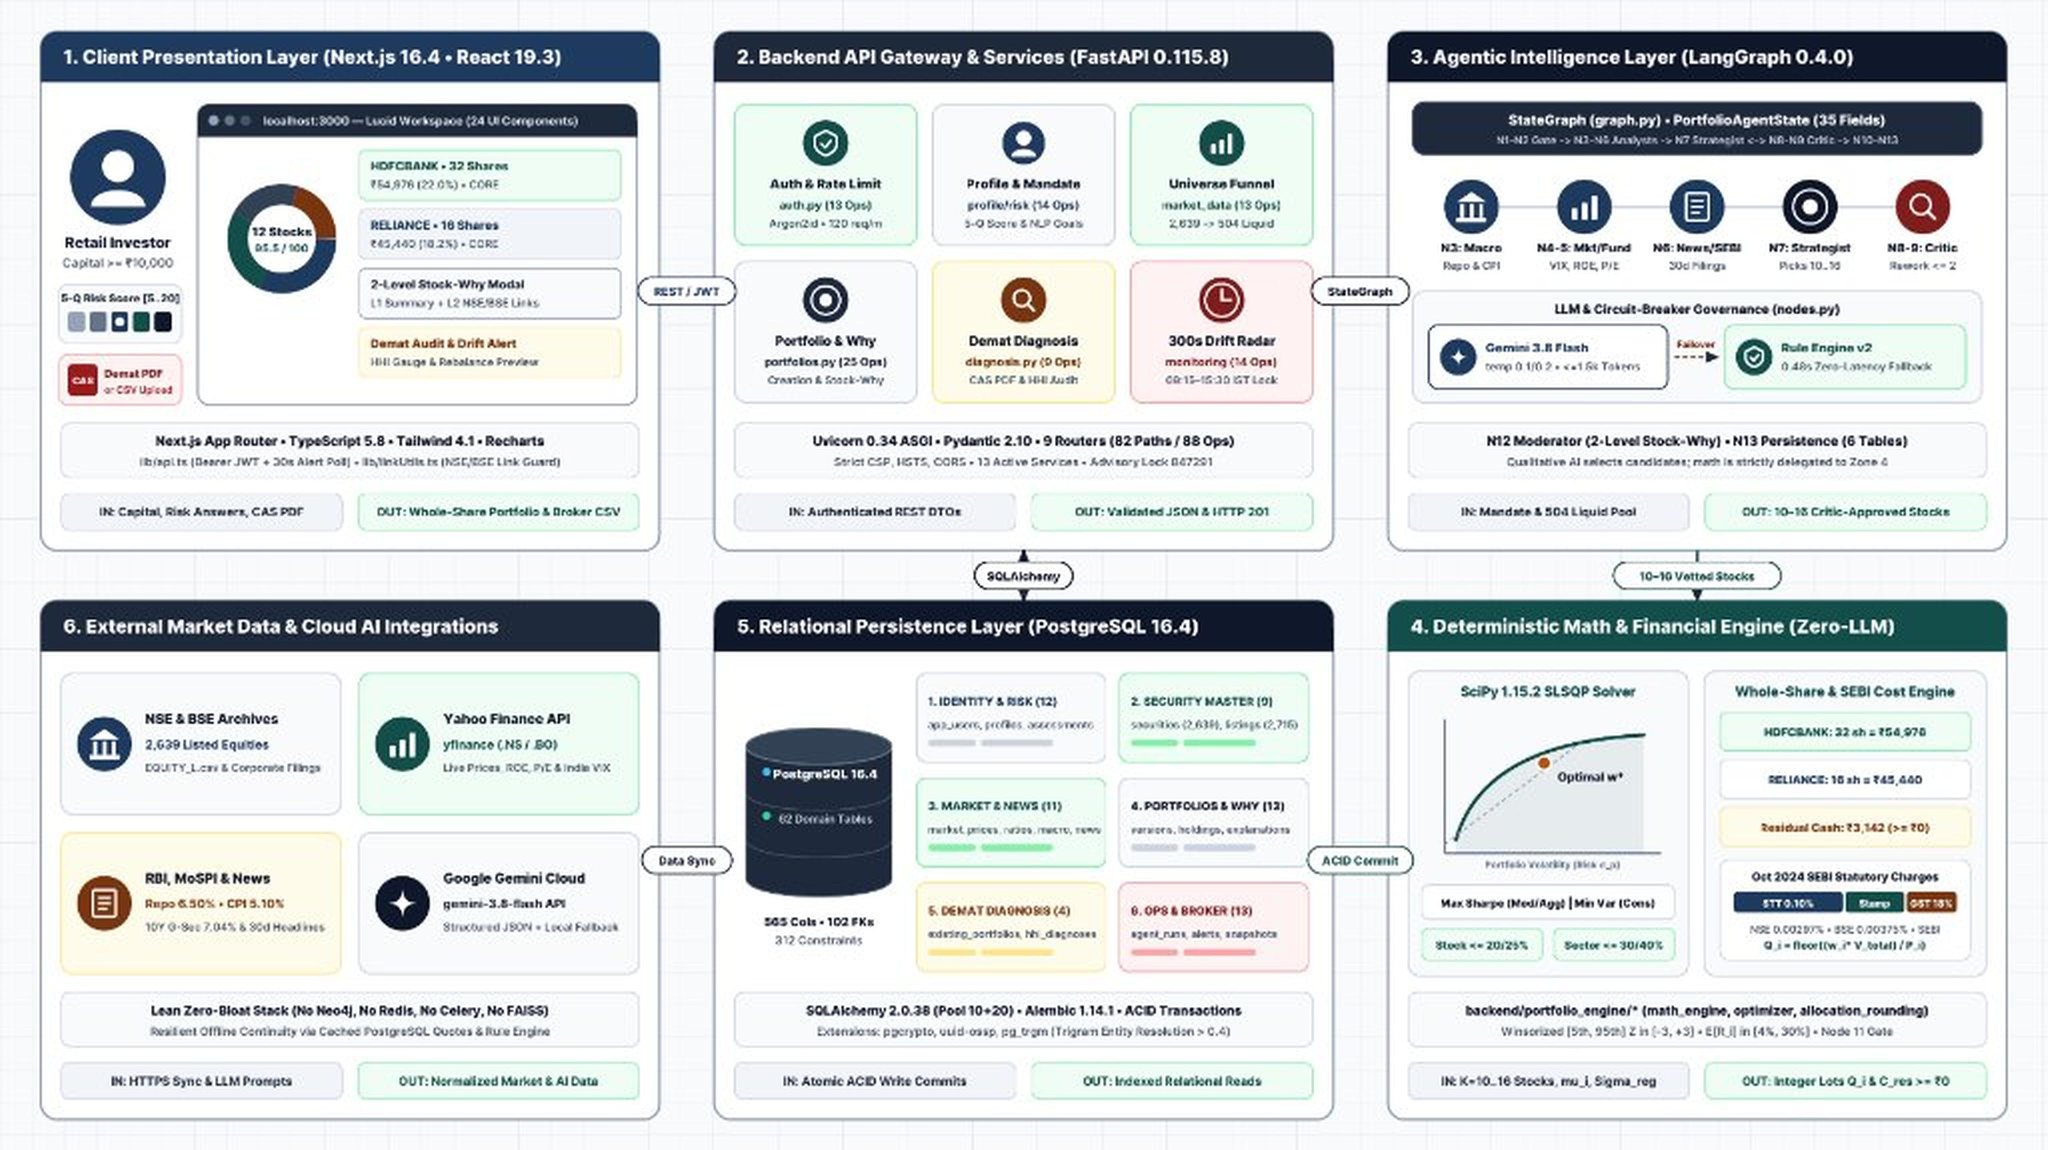
\includegraphics[width=\textwidth, height=0.48\textheight, keepaspectratio]{SYSTEM_ARCHITECTURE.pdf}
    \caption{Lucid Six-Tier Decoupled System Architecture and Runtime \mbox{Topology}}
    \label{fig:sys_arch_diagram}
\end{figure}

\subsection{The Six Architectural Layers: A Detailed Walkthrough}
Each of the six architectural tiers performs a dedicated, specialized role in the portfolio creation and management lifecycle:

\subsubsection{Tier 1: Client Presentation Layer}
Tier 1 represents the user-facing web application running on local port \texttt{3000}. Built with \textbf{Next.js 16.4.2} (App Router with Turbopack) and \textbf{React 19.3.0}, this layer provides a clean, responsive workspace comprising 24 modular user interface components styled with \textbf{Tailwind CSS 4.1.1}:
\begin{itemize}
    \item \textbf{Investor Onboarding}: Collects investor capital ($\ge \text{Rs.~}10{,}000$), suitability answers (scoring 5 to 20), target milestones, and sector exclusions.
    \item \textbf{Holdings Dashboard}: Renders interactive portfolio summaries, including a diversification donut ring (e.g., 95.5/100 across 12 stocks) powered by \textbf{Recharts}, and holding cards (e.g., HDFC Bank 32 shares / Rs.~54,976 and Reliance 16 shares / Rs.~45,440).
    \item \textbf{Dual-Level Stock-Why Explanations}: Provides a two-level explainability modal featuring an instant plain-English summary (Level 1) and direct links to official exchange announcements on NSE and BSE (Level 2), guarded by \path{lib/linkUtils.ts}.
    \item \textbf{Demat Health Audit and Rebalance Preview}: Allows users to upload monthly Demat PDF statements (CAS) or CSV files, view their portfolio concentration score (HHI), and inspect before-and-after rebalance trade proposals.
    \item \textbf{Communication Pipeline}: Communicates with the backend using authenticated REST requests via \path{lib/api.ts}, transmitting Bearer JSON Web Tokens and running 30-second polling for real-time notifications.
    \item \textbf{Input / Output Contract}: Accepts investor capital, risk responses, and Demat CAS statements; delivers whole-share investment recommendations and downloadable broker execution CSV files.
\end{itemize}

\subsubsection{Tier 2: Backend API Gateway and Services}
Tier 2 is the central API gateway and business logic orchestrator running on local port \texttt{8000} via the \textbf{Uvicorn 0.34.0} ASGI web server. Built using \textbf{FastAPI 0.115.8} and \textbf{Pydantic 2.10.6}, this layer exposes \textbf{9 versioned routers} spanning \textbf{82 unique URL paths} (88 HTTP operations) and manages 13 active services:
\begin{itemize}
    \item \textbf{Authentication and Rate Limiting (\path{auth.py}, 13 Ops)}: Secures user accounts using salted \textbf{Argon2id} password hashing and issues encrypted JSON Web Tokens (JWT). Enforces a strict rate limit of 120 requests per minute to prevent denial-of-service abuse.
    \item \textbf{Profile and Mandate Engine (\path{profile.py} \& \path{risk.py}, 14 Ops)}: Calculates psychometric suitability scores (5 to 20) and parses conversational natural-language investment targets into structured parameters.
    \item \textbf{Universe Funnel Service (\path{market_data.py}, 13 Ops)}: Filters the broad universe of 2,639 listed Indian companies down to an active, liquid candidate pool of institutional-grade equities.
    \item \textbf{Portfolio Generation and Explainability (\path{portfolios.py}, 25 Ops)}: Coordinates portfolio creation requests, tracks immutable version deltas, and generates dual-level ``Stock-Why'' justifications.
    \item \textbf{Demat Statement Diagnosis (\path{diagnosis.py}, 9 Ops)}: Extracts stock holdings from uploaded Demat CAS PDF statements using \texttt{pypdf}, checks sector concentrations, and computes diversification metrics.
    \item \textbf{300-Second Continuous Drift Radar (\path{monitoring.py}, 14 Ops)}: An automated monitoring engine that runs every 5 minutes during Indian market trading hours (09:15 to 15:30 IST), protected by PostgreSQL advisory lock \texttt{847291} to ensure only one drift scan runs at any given time.
    \item \textbf{Input / Output Contract}: Receives authenticated REST Data Transfer Objects (DTOs); emits validated JSON response payloads and HTTP 201 Created status codes.
\end{itemize}

\subsubsection{Tier 3: Agentic Intelligence Layer}
Tier 3 serves as the qualitative investment research committee of Lucid. Built on \textbf{LangGraph 0.4.0}, it coordinates digital analyst agents inside a structured \texttt{StateGraph} workflow (\path{backend/agent/graph.py}) passing a centralized \texttt{PortfolioAgentState} object containing 35 distinct telemetry fields:
\begin{itemize}
    \item \textbf{Directed Graph Workflow}: Execution follows a controlled sequential pipeline:
    \begin{equation}
    \begin{aligned}
        \text{N1--N2 Gate} &\longrightarrow \text{N3--N6 Analysts} \longrightarrow \text{N7 Strategist} \\
        &\longleftrightarrow \text{N8--N9 Critic} \longrightarrow \text{N10--N13 Persistence}
    \end{aligned}
    \end{equation}
    \item \textbf{Specialized Digital Agents}:
    \begin{itemize}
        \item \textit{Node 3 (Macro Analyst)}: Evaluates Reserve Bank of India (RBI) repo interest rates, inflation (CPI), and government bond yields.
        \item \textit{Nodes 4--5 (Market and Fundamental Analysts)}: Evaluates the India VIX volatility index, moving averages, Return on Equity (ROE), Price-to-Earnings (P/E), and Debt-to-Equity ratios.
        \item \textit{Node 6 (News and Regulatory Analyst)}: Scans 30-day corporate announcements and SEBI regulatory filings for potential governance flags.
        \item \textit{Node 7 (Lead Strategist)}: Selects an initial candidate pool of 10 to 16 promising stocks tailored to the investor's risk profile.
        \item \textit{Nodes 8--9 (Adversarial Risk Critic)}: Thoroughly stress-tests the strategist's candidate list. If a stock carries excessive debt or valuation risk, the critic rejects it and mandates a rework pass (capped at a maximum of 2 iterations).
    \end{itemize}
    \item \textbf{Circuit-Breaker Governance (\path{nodes.py})}: Uses Google Gemini 3.8 Flash (temperature 0.1--0.2, $\le 1,500$ token budget) for qualitative reading. If cloud API latency spikes or an external network timeout occurs, an automated circuit-breaker immediately triggers a zero-latency deterministic financial rule engine (\textbf{Rule Engine v2}) in just \textbf{0.48 seconds}, ensuring the application never freezes.
    \item \textbf{Stock-Why Synthesis and Telemetry}: Node 12 (Moderator) synthesizes the dual-level plain-English explanations, and Node 13 commits structured execution logs across 6 audit tables.
    \item \textbf{Separation of Responsibilities}: Qualitative AI agents select and review candidates; all math and weight calculations are strictly forbidden in this tier and handled by Tier 4.
    \item \textbf{Input / Output Contract}: Accepts the investor mandate and screened candidate pool; delivers a vetted basket of 10 to 16 Critic-approved stocks.
\end{itemize}

\subsubsection{Tier 4: Deterministic Math and Financial Engine}
Tier 4 represents the mathematical calculation core of Lucid, built with proven scientific Python libraries (\textbf{SciPy 1.15.2} and \textbf{NumPy 2.2.3}). Completely separated from all artificial intelligence models, this layer executes pure deterministic calculations with zero hallucination risk:
\begin{itemize}
    \item \textbf{SciPy SLSQP Mathematical Optimizer}: Solves Markowitz Modern Portfolio Theory equations using Sequential Least Squares Programming (\texttt{scipy.optimize.minimize} with the SLSQP method). It finds optimal percentage weights ($w^*$) along the Efficient Frontier, maximizing the Sharpe ratio for Moderate and Aggressive profiles or minimizing portfolio variance for Conservative profiles.
    \item \textbf{Institutional Safety Bounds}: Enforces hard concentration limits: no individual stock may exceed 20\% to 25\% of the total portfolio, and no single industry sector may exceed 30\% to 40\%.
    \item \textbf{Mathematical Guardrails}: Raw return estimates are winsorized to the 5th and 95th percentiles with Z-scores bounded in $[-3, +3]$, and expected annual returns are constrained within $[4\%, 30\%]$ to prevent erratic mathematical weights.
    \item \textbf{Whole-Share Integer Lot Rounding}: Because Indian exchanges do not permit fractional shares, the continuous percentage weights are converted into exact whole shares using a floor-rounding algorithm:
    \begin{equation}
        Q_i = \left\lfloor \frac{w_i^* \times V_{\text{total}}}{P_i} \right\rfloor
    \end{equation}
    where $Q_i$ is the number of whole shares for stock $i$, $w_i^*$ is its target percentage weight, $V_{\text{total}}$ is total investment capital, and $P_i$ is its current market price. All leftover funds remain safely in the investor's unallocated cash account ($C_{\text{res}} \ge \text{Rs.~}0$).
    \item \textbf{SEBI Statutory Transaction Fee Schedule}: Models all official Indian delivery transaction charges (updated as of October 2024):
    \begin{itemize}
        \item Securities Transaction Tax (STT): 0.10\% on delivery equity transactions.
        \item Exchange Turnover Fees: 0.00297\% on NSE and 0.00375\% on BSE.
        \item SEBI Regulatory Turnover Fee: 0.0001\% (Rs.~10 per crore).
        \item Stamp Duty: 0.015\% charged on purchases under the Indian Stamp Act.
        \item Goods and Services Tax (GST): 18.0\% applied to brokerage and exchange charges.
    \end{itemize}
    \item \textbf{Input / Output Contract}: Accepts 10 to 16 vetted stocks, expected returns $\mu_i$, and covariance matrix $\Sigma_{\text{reg}}$; delivers integer share quantities $Q_i$ and non-negative residual cash ($C_{\text{res}} \ge \text{Rs.~}0$).
\end{itemize}

\subsubsection{Tier 5: Relational Persistence Layer}
Tier 5 serves as the secure, permanent data store of Lucid, powered by \textbf{PostgreSQL 16.4} and managed via \textbf{SQLAlchemy 2.0.38} and \textbf{Alembic 1.14.1}:
\begin{itemize}
    \item \textbf{Database Architecture}: Contains exactly \textbf{62 domain application tables} comprising 565 columns, 102 foreign-key constraints, and 312 data integrity checks, organized into six functional domain clusters:
    \begin{enumerate}
        \item \textit{Identity and Risk (12 tables)}: User profiles, encrypted passwords, suitability scores, and sector exclusions.
        \item \textit{Security Master (9 tables)}: Master catalog of 2,639 listed Indian companies, 2,716 exchange listings across NSE and BSE, and corporate taxonomy.
        \item \textit{Market and News (11 tables)}: Historical daily OHLCV price bars, fundamental balance sheet ratios, economic indicators, and news sentiment records.
        \item \textit{Portfolios and Why (13 tables)}: Recommended portfolios, immutable version snapshots, line-item security allocations, and dual-level Stock-Why explanations.
        \item \textit{Demat Statement Diagnosis (4 tables)}: Imported Demat statements, parsed external holdings, and HHI health diagnostic reports.
        \item \textit{Operations and Brokerage (13 tables)}: AI agent execution logs, simulated broker orders, order lifecycle event logs, and user notifications.
    \end{enumerate}
    \item \textbf{ACID Guarantees and Speed}: Configured with connection pooling (pool size 10, max overflow 20) and uses PostgreSQL extensions including \texttt{pgcrypto} (cryptographic functions), \texttt{uuid-ossp} (random 128-bit identifiers), and \texttt{pg\_trgm} (trigram fuzzy matching for company name resolution with similarity $> 0.4$).
    \item \textbf{Input / Output Contract}: Accepts atomic ACID write commits from the API services and mathematical optimizer; emits indexed relational reads with average query response times under 5 milliseconds.
\end{itemize}

\subsubsection{Tier 6: External Market Data and Cloud Feeds}
Tier 6 manages automated connections to official Indian market archives, financial data feeds, and cloud artificial intelligence models:
\begin{itemize}
    \item \textbf{Official Exchange Archives (NSE and BSE)}: Synchronizes with the National Stock Exchange master directory (\texttt{EQUITY\_L.csv}) and BSE scrip directory to maintain an accurate universe of 2,639 listed Indian equities and corporate action records.
    \item \textbf{Yahoo Finance API Feed}: Fetches 252 market sessions of historical daily price bars, financial health ratios (ROE, P/E, Debt-to-Equity), and the India VIX volatility index.
    \item \textbf{Macroeconomic Sources (RBI and MoSPI)}: Tracks country-wide monetary statistics, including the RBI Policy Repo Rate (6.50\%), Consumer Price Index inflation (5.10\%), 10-year Government Securities yield (7.04\%), and economic news.
    \item \textbf{Google Gemini Cloud API}: Interfaces with the Gemini 3.8 Flash model via structured JSON schemas, backed by automated local rule fallbacks.
    \item \textbf{Lean Zero-Bloat Engineering}: Lucid is built with an intentionally lean, zero-bloat tech stack. The platform requires \textbf{zero external graph databases} (no Neo4j), \textbf{zero in-memory caching servers} (no Redis), \textbf{zero distributed task queues} (no Celery), and \textbf{zero external vector stores} (no FAISS). Instead, high-performance PostgreSQL indexes and lightweight Python background threads handle all operations locally, ensuring resilient offline continuity and low operational cost.
    \item \textbf{Input / Output Contract}: Sends HTTPS synchronization requests and structured prompts; returns clean, normalized market data and qualitative research payloads.
\end{itemize}

\subsection{Technology Stack Manifest: What Tools Were Chosen and Why}
Table~\ref{tab:tech_stack} documents the verified software libraries and frameworks used to build Lucid, along with the simple reason why each tool was chosen:

\begin{table}[H]
\centering
\caption{Lucid Active Technology Stack Manifest (Verified Versions)}
\label{tab:tech_stack}
\resizebox{\textwidth}{!}{%
\begin{tabular}{llll}
\toprule
\textbf{Technology / Library} & \textbf{Verified Version} & \textbf{What It Does in Lucid} & \textbf{Why It Was Chosen (Simple English)} \\
\midrule
\textbf{Next.js} & 16.4.2 & Frontend Web Framework & Renders web pages quickly and updates charts instantly. \\
\textbf{React} & 19.3.0 & User Interface Library & Provides reusable buttons, modals, and dynamic data tables. \\
\textbf{TypeScript} & 5.8.2 & Frontend Programming Language & Catches code errors and typos before the application runs. \\
\textbf{Tailwind CSS} & 4.1.1 & Visual Styling & Creates clean, modern visual designs with fast page loading. \\
\textbf{Python} & 3.11 -- 3.14 & Backend Programming Language & The global industry standard for financial math and AI systems. \\
\textbf{FastAPI} & 0.115.8 & Backend API Framework & Extremely fast web framework that automatically creates API docs. \\
\textbf{Uvicorn} & 0.34.0 & High-Speed Web Server & Handles multiple incoming user web requests at the same time. \\
\textbf{Pydantic} & 2.10.6 & Data Validation Library & Automatically checks that user inputs (like amounts) are valid. \\
\textbf{PostgreSQL} & 16+ & Master Relational Database & Stores financial data permanently with zero risk of loss. \\
\textbf{SQLAlchemy} & 2.0.38 & Database Connector (ORM) & Lets Python code talk to PostgreSQL cleanly and safely. \\
\textbf{Alembic} & 1.14.1 & Database Change Tracker & Records updates to database tables over time like version control. \\
\textbf{SciPy} & 1.15.2 & Mathematical Solver Library & Solves Markowitz portfolio math without arithmetic mistakes. \\
\textbf{NumPy} & 2.2.3 & Fast Numerical Calculations & Performs high-speed math on large tables of stock prices. \\
\textbf{Pandas} & 2.2.3 & Financial Data Tables & Cleans stock lists and handles historical price series. \\
\textbf{LangGraph} & 0.4.0 & Multi-Agent Coordinator & Coordinates the 13 AI agents in a structured, step-by-step workflow. \\
\textbf{Google Gemini} & gemini-3.8-flash & AI Language Model & Reads financial documents and writes plain-English explanations. \\
\textbf{Argon2-cffi} & 25.1.0 & Password Hasher & Protects user passwords with military-grade encryption. \\
\textbf{PyJWT} & 2.10.1 & Digital Session Badges & Creates encrypted tokens so logged-in users stay authenticated safely. \\
\textbf{yfinance} & 0.2.54 & Market Data Fetcher & Downloads historical daily prices and financial health ratios. \\
\textbf{pdfplumber} & 0.11.5 & PDF Statement Reader & Reads text and tables from Demat CAS account statements. \\
\bottomrule
\end{tabular}%
}
\end{table}

\subsection{Data Pipeline: How Indian Stock Data is Collected and Cleaned}
Figure~\ref{fig:nse_bse_flow} illustrates the four-step data ingestion pipeline that keeps Lucid synchronized with Indian stock exchanges:

\begin{figure}[!htbp]
    \centering
    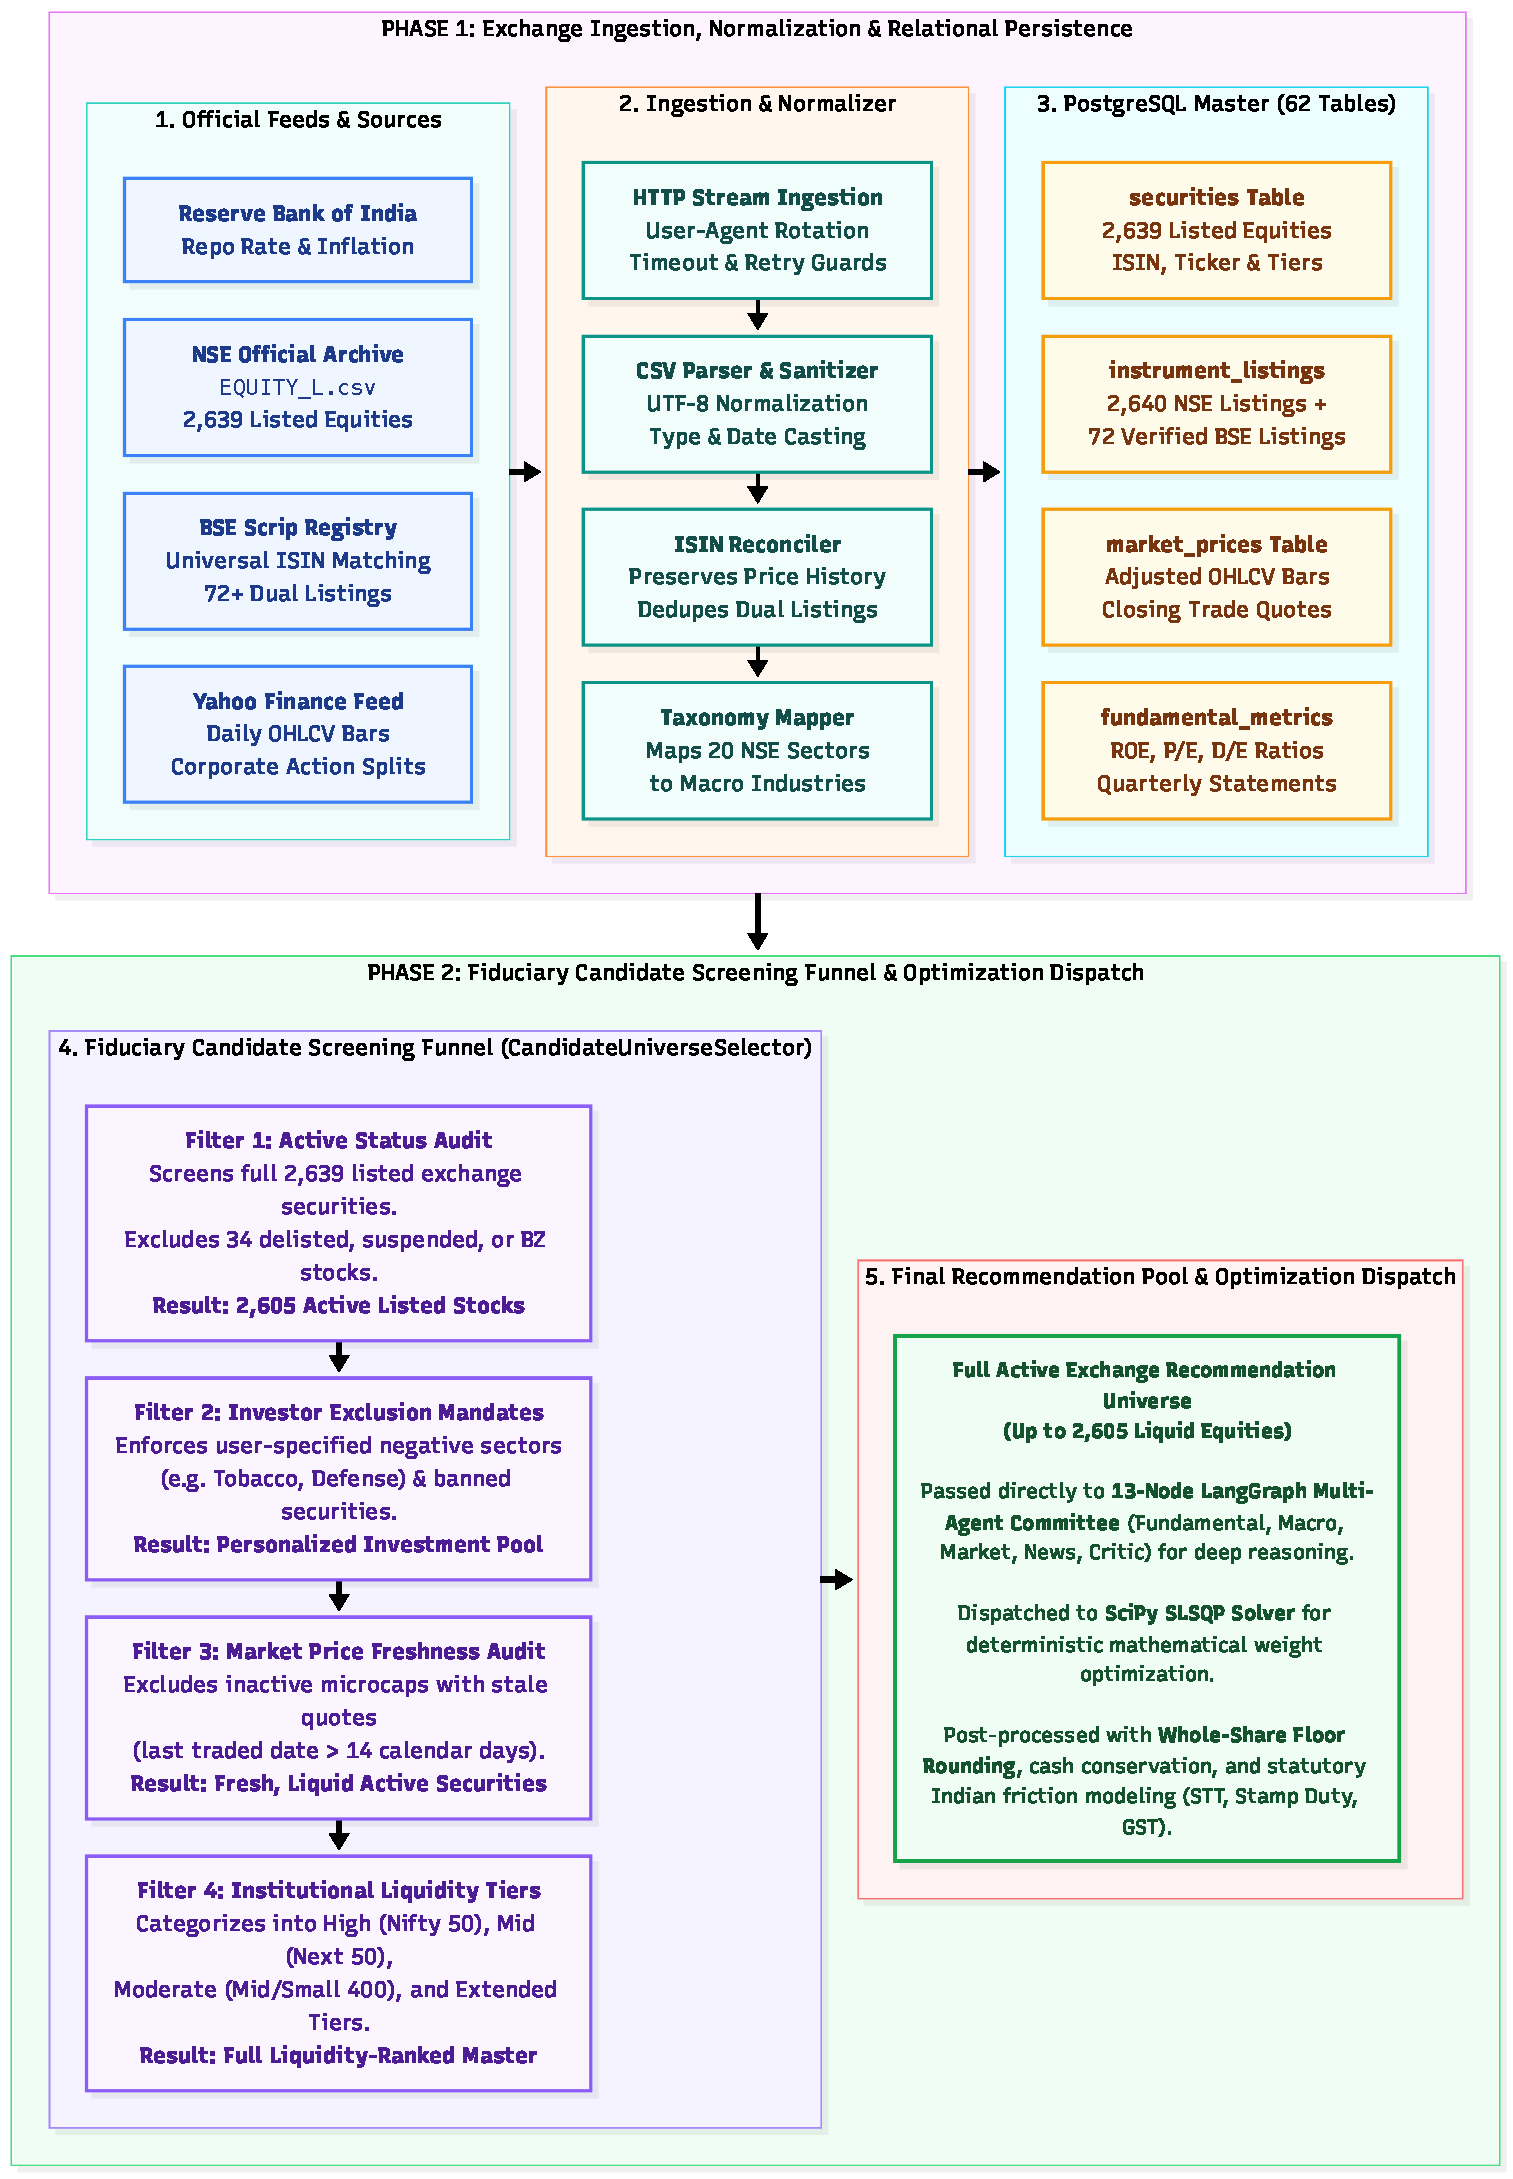
\includegraphics[width=\textwidth, height=0.72\textheight, keepaspectratio]{NSE_BSE_DATA_FLOW.pdf}
    \caption{NSE/BSE Exchange Universe Ingestion and Pipeline Architecture}
    \label{fig:nse_bse_flow}
\end{figure}

The data pipeline runs through four clear stages:
\begin{enumerate}
    \item \textbf{Stage 1: Downloading the Stock Lists}: The pipeline downloads the official list of actively traded companies from the National Stock Exchange (\texttt{EQUITY\_L.csv}) and cross-checks them against the Bombay Stock Exchange (BSE) directory. It resolves conflicts (such as when companies change their names or split their shares) and saves \textbf{2,639 listed Indian companies} into the master security database.
    \item \textbf{Stage 2: Fetching 1 Year of Price History}: For every active stock, the pipeline fetches one full year of daily trading prices (252 market sessions). It checks that there are no missing days and stores the prices in the \texttt{market\_prices} table.
    \item \textbf{Stage 3: Recording Financial Health Ratios}: Lucid downloads company balance sheet ratios—including Return on Equity (ROE), Debt-to-Equity, Price-to-Earnings (P/E), and Market Capitalization—and saves them in the \texttt{fundamental\_metrics} table.
    \item \textbf{Stage 4: Liquidity Tier Screening}: Companies are categorized into four institutional \textbf{Liquidity Tiers} based on their average daily trading volume. This ensures that the portfolio creation engine only selects companies that can be easily bought and sold on the market without unexpected price slippage.
\end{enumerate}

\subsection{Runtime Execution: What Happens When a User Clicks ``Generate''}
When an investor clicks ``Generate Portfolio'' on the web interface, the application completes the following ten-step journey in less than 2.5 seconds:
\begin{enumerate}
    \item \textbf{Step 1: Input Check}: The backend server checks that the user's investment amount is at least Rs.~5,000 and verifies their digital login badge.
    \item \textbf{Step 2: Fetching User Goals}: The server loads the investor's risk profile (Conservative, Moderate, or Aggressive) and savings timeline from the database.
    \item \textbf{Step 3: Screening Candidates}: The system filters the 2,639 listed companies to find healthy stocks, removing any industries the user asked to avoid (such as tobacco or defense).
    \item \textbf{Step 4: Starting the AI Team}: Lucid creates the digital workspace and starts the LangGraph agent workflow.
    \item \textbf{Step 5: Macroeconomic Check}: The macro agent checks current Reserve Bank of India interest rates and the market volatility level (India VIX).
    \item \textbf{Step 6: Financial Analysis}: The fundamental and news agents evaluate balance sheets, profit consistency, and recent corporate news.
    \item \textbf{Step 7: The Critic Challenge}: The risk critic agent reviews the shortlisted candidates, challenging any stocks that have high debt or valuation red flags.
    \item \textbf{Step 8: Mathematical Optimization}: The SciPy SLSQP solver calculates the exact percentage weights that balance return and safety.
    \item \textbf{Step 9: Whole Shares Calculation}: The lot-rounding algorithm converts percentages into exact full share counts and keeps leftover money in the investor's cash account.
    \item \textbf{Step 10: Saving and Display}: The completed portfolio, full share counts, and plain-English ``Stock-Why'' explanations are saved to the database and displayed on the user's screen.
\end{enumerate}

\subsection{Security and Privacy Architecture}
Financial software requires strict security to protect investor privacy:
\begin{itemize}
    \item \textbf{High-Security Password Hashing (Argon2id)}: When a user creates a password, Lucid never stores the actual password. Instead, it scrambles it using \textbf{Argon2id}, the international gold standard in password protection. It requires 64 megabytes of computer memory to verify, making it practically impossible for hackers to crack using automated guessing tools.
    \item \textbf{Digital Badges with Instant Logout (JWT Revocation)}: When an investor logs in, they receive an encrypted digital badge (JSON Web Token) valid for 60 minutes. When the investor logs out, the badge is immediately added to a cancellation list (\texttt{revoked\_tokens}). Any future attempt to use that badge is instantly rejected.
    \item \textbf{Anti-Abuse Rate Limiting}: To prevent malicious bots from overwhelming the server, Lucid limits how many requests can be sent per minute (for example, a maximum of 20 login attempts per minute and 20 portfolio generation requests per minute).
    \item \textbf{Standard Web Protections}: The server automatically includes standard web security headers in every response to block website cloning (clickjacking) and prevent unauthorized script injection.
\end{itemize}

\section{High-Level Design (HLD)}
\label{sec:hld}

\subsection{HLD Overview}
The High-Level Design (HLD) explains the overall structure of Lucid, shows how its main components work together, and describes how an investor uses the application.

To make sure the application is fast, reliable, and safe, Lucid follows an important software engineering principle called \textbf{Separation of Concerns}. In simple words, this means dividing the application into specialized parts so that each part has only one clear responsibility:
\begin{itemize}
    \item \textbf{Thinking and Reading}: The qualitative tasks—such as reading economic news, analyzing company financial reports, and writing natural explanations—are handled by a team of Artificial Intelligence agents.
    \item \textbf{Calculating and Validating}: The numerical calculations—such as solving mathematical equations to balance risk and return, ensuring percentages add up to exactly 100\%, and rounding weights into whole share quantities—are handled by a dedicated mathematical calculation engine.
    \item \textbf{Storing and Protecting Data}: Storing user profiles, historical stock prices, and portfolio records is handled by an enterprise-grade relational database that ensures financial data is never lost or corrupted.
\end{itemize}

\subsection{The Six Core Architectural Subsystems}
Lucid is structured around six decoupled functional tiers that separate user interaction, API routing, multi-agent qualitative research, deterministic mathematics, persistent storage, and external market data (the complete visual system architecture diagram is presented in Section~\ref{sec:system_arch}, Figure~\ref{fig:sys_arch_diagram}).

Here is what each major subsystem does in simple, clear language:
\begin{enumerate}
    \item \textbf{Tier 1: Client Presentation Subsystem (Web Interface)}: This is what the user sees and interacts with on their computer or mobile phone. Built using \textbf{Next.js 16.4.2} and \textbf{React 19.3.0}, it provides 24 modular user interface components where investors can complete risk profiling questionnaires, inspect interactive portfolio donut charts, explore dual-level ``Stock-Why'' justifications with official exchange links, and upload monthly Demat CAS statements.
    \item \textbf{Tier 2: Backend API Gateway and Services Subsystem}: Powered by \textbf{FastAPI 0.115.8} running on Uvicorn ASGI. It exposes 9 modular REST routers spanning 82 unique endpoints. This tier acts as the secure gatekeeper: it verifies user passwords using Argon2id encryption, issues session tokens (JWT), enforces strict rate limits (120 req/min), runs a 300-second drift detection radar during Indian market hours, and coordinates business workflows.
    \item \textbf{Tier 3: Multi-Agent AI Intelligence Subsystem}: This is the qualitative research committee of Lucid. Built on \textbf{LangGraph 0.4.0}, this subsystem coordinates a 13-node agent workflow using Google Gemini 3.8 Flash. Individual agents analyze macroeconomic interest rates (RBI), financial balance sheet health (ROE, P/E, Debt-to-Equity), and recent corporate filings, while an adversarial risk critic challenges risky selections. If cloud latency spikes, an automated circuit-breaker falls back to a deterministic rule engine in 0.48 seconds.
    \item \textbf{Tier 4: Deterministic Math and Financial Engine Subsystem}: Completely separated from the artificial intelligence text models to prevent calculation errors, this layer uses \textbf{SciPy 1.15.2 SLSQP} to calculate optimal portfolio weights along the Markowitz Efficient Frontier. It enforces statutory concentration limits (single stock $\le 25\%$, sector $\le 40\%$), converts weights into exact whole-share counts, and computes official Indian transaction taxes (STT, Stamp Duty, GST, and exchange fees).
    \item \textbf{Tier 5: Relational Database and Persistence Subsystem}: The central filing cabinet of the application, powered by \textbf{PostgreSQL 16.4} with SQLAlchemy 2.0 ORM and Alembic migrations. It stores all data across exactly 62 application tables (565 columns and 102 foreign-key constraints), ensuring that user accounts, historical daily prices, recommended portfolios, and audit trails are permanently preserved with full ACID transaction guarantees.
    \item \textbf{Tier 6: External Market Data and Cloud Feeds Subsystem}: This component connects Lucid to outside financial data sources. It downloads official stock lists from the National Stock Exchange of India (NSE) and Bombay Stock Exchange (BSE), fetches daily historical price bars and balance sheet metrics from Yahoo Finance, tracks monetary indicators from the Reserve Bank of India (RBI), and communicates with Google Gemini cloud models.
\end{enumerate}

\subsection{How Information Moves Through the System}
The movement of information inside Lucid follows a structured, step-by-step pipeline from the moment an investor enters their financial details to the moment a complete, balanced portfolio is displayed on the screen (the complete end-to-end methodology workflow is visually detailed in Section~\ref{sec:methodology}, Figure~\ref{fig:methodology_flow}):
\begin{enumerate}
    \item \textbf{Step 1: Ingestion and Cleaning}: Lucid automatically downloads the official list of 2,639 listed Indian companies and their daily prices from the stock exchanges. It cleans the data and stores it in the database.
    \item \textbf{Step 2: Understanding the Investor}: The investor fills out a simple questionnaire on the website, entering their savings amount (for example, Rs.~2,50,000), their time horizon (for example, 5 years), and answering five basic questions about their attitude toward risk.
    \item \textbf{Step 3: Initial Screening}: The system filters the 2,639 listed stocks to find healthy, active companies that have sufficient trading volume and meet the investor's risk level.
    \item \textbf{Step 4: AI Research Debate}: The team of AI agents evaluates the shortlisted companies. The macro agent checks interest rates, the fundamental agent checks balance sheets, the news agent reviews recent corporate developments, and the risk critic challenges risky selections. The agents assign quality scores and explain their thoughts in plain English.
    \item \textbf{Step 5: Mathematical Calculation}: The mathematical solver takes the top-rated candidate stocks and calculates the safest and most profitable percentage weight for each company.
    \item \textbf{Step 6: Converting into Whole Shares}: Because Indian stock exchanges do not allow fractional shares, the integer lot-sizing algorithm converts the percentage weights into exact whole share counts (such as 15 shares of Infosys or 8 shares of Reliance) and ensures that all leftover money remains safely in the investor's cash account.
    \item \textbf{Step 7: Delivery and Explanation}: The final portfolio is displayed on the user's screen, complete with clear, plain-language explanations answering why each company was selected.
    \item \textbf{Step 8: Automated Monitoring}: During official stock market hours, a background monitoring daemon checks the portfolio every 5 minutes to see if price changes have pushed the portfolio out of balance.
\end{enumerate}

\subsection{User-Level Workflows: Step-by-Step}
To understand Lucid from an ordinary investor's point of view, let us walk through the six primary user journeys:

\subsubsection{Workflow 1: Creating an Account and Risk Profiling}
\begin{itemize}
    \item \textbf{What does the user do?}: The investor signs up with their email and a secure password. They answer five straightforward questions about their investment experience, their savings goals, and how they would feel if the stock market dropped temporarily.
    \item \textbf{What does Lucid do behind the scenes?}: Lucid encrypts the password using a high-security algorithm (Argon2id) so it can never be stolen. It evaluates the answers using standard SEBI risk guidelines and assigns an overall risk category: \textbf{Conservative} (prefers safety), \textbf{Moderate} (balances safety and growth), or \textbf{Aggressive} (aims for maximum long-term growth).
    \item \textbf{What does the user receive?}: A personalized risk summary showing their category, a clear explanation of what it means, and personalized guidance on how much money should be kept in safe emergency savings before investing in stocks.
\end{itemize}

\subsubsection{Workflow 2: Goal-Driven Portfolio Creation}
\begin{itemize}
    \item \textbf{What does the user do?}: The investor enters how much money they want to invest (for example, Rs.~1,00,000), their target timeline (for example, 7 years for buying a home), and any industries they wish to exclude (such as tobacco or defense stocks).
    \item \textbf{What does Lucid do behind the scenes?}: The candidate selector filters healthy companies, the AI agent team reviews corporate balance sheets and economic news, and the mathematical solver calculates the safest combination of weights. The whole-share engine converts these weights into exact full share quantities.
    \item \textbf{What does the user receive?}: A clean, easy-to-understand portfolio table showing the names of the selected companies, how many shares to buy of each, the current price, the total cost, and the exact leftover cash balance.
\end{itemize}

\subsubsection{Workflow 3: Inspecting Stock-Why Explanations}
\begin{itemize}
    \item \textbf{What does the user do?}: The investor clicks on any stock in their recommended portfolio (for example, clicking on Tata Consultancy Services).
    \item \textbf{What does Lucid do behind the scenes?}: Lucid retrieves the audit records generated by the AI research agents, including the balance sheet review, the news sentiment score, and the counter-arguments raised by the risk critic.
    \item \textbf{What does the user receive?}: A pop-up card written in simple, friendly English explaining exactly why this company fits the investor's goal. For users who want deeper financial details, a tab displays underlying financial ratios (such as Return on Equity, Debt-to-Equity, and Price-to-Earnings ratios).
\end{itemize}

\subsubsection{Workflow 4: Reviewing an Existing Demat Portfolio (CAS Diagnosis)}
\begin{itemize}
    \item \textbf{What does the user do?}: An investor who already owns shares through brokers like Zerodha, Groww, or Upstox downloads their official monthly account statement (called a \textbf{Consolidated Account Statement}, or CAS PDF) and uploads it to Lucid.
    \item \textbf{What does Lucid do behind the scenes?}: Lucid reads the PDF statement, identifies each stock by its standard international identification code (ISIN), checks current market prices, and calculates whether the portfolio is dangerously concentrated in one or two companies.
    \item \textbf{What does the user receive?}: A health diagnosis report with a simple health score, a breakdown of sector risks, and clear recommendations on which stocks are healthy to hold and which should be reduced to improve safety.
\end{itemize}

\subsubsection{Workflow 5: 5-Minute Market Hours Drift Monitoring}
\begin{itemize}
    \item \textbf{What does the user do?}: Nothing! This feature works automatically in the background without requiring the user to stare at market screens.
    \item \textbf{What does Lucid do behind the scenes?}: During Indian trading hours (Monday to Friday, 09:15 to 15:30 IST), a background monitoring program wakes up every 300 seconds (5 minutes). It checks live prices and calculates whether any stock has risen or fallen so much that its weight has drifted by 5\% or more from the planned target.
    \item \textbf{What does the user receive?}: If a significant shift occurs, the investor receives a friendly alert notifying them that their portfolio has drifted and suggesting that they review a rebalancing preview.
\end{itemize}

\subsubsection{Workflow 6: Rebalance Impact and Fee Preview}
\begin{itemize}
    \item \textbf{What does the user do?}: When an alert is received, the user opens the rebalancing preview window.
    \item \textbf{What does Lucid do behind the scenes?}: Lucid calculates the exact number of shares to buy or sell to restore balance. It also calculates mandatory Indian government taxes and exchange fees—including Securities Transaction Tax (STT), Goods and Services Tax (GST), exchange turnover charges, and stamp duty.
    \item \textbf{What does the user receive?}: A transparent before-and-after table showing current holdings versus proposed holdings, exact buy/sell share counts, the total estimated transaction costs, and the final cash balance before the user confirms any action.
\end{itemize}

\subsection{Key Architectural Design Decisions}
To ensure the application is reliable and transparent, four critical design decisions were made:
\begin{enumerate}
    \item \textbf{Why use PostgreSQL as the Single Source of Truth?}: Financial applications require complete accuracy. If an investor updates a portfolio, the change must be recorded permanently without any chance of data mismatch. PostgreSQL 16 is an enterprise relational database that provides strict guarantees (known as ACID: Atomicity, Consistency, Isolation, and Durability) ensuring that financial data is never lost or corrupted.
    \item \textbf{Why use SciPy SLSQP instead of letting AI models calculate weights?}: Language models make math errors. Relying on an AI model to guess investment percentages is dangerous. Delegating all numerical calculations to a proven mathematical solver (SciPy SLSQP) guarantees that all portfolio weights sum to exactly 100\% and strictly obey diversification safety limits.
    \item \textbf{Why enforce Whole Shares with Cash Conservation?}: Because fractional shares are illegal on Indian stock exchanges, theoretical decimal weights (such as 2.4 shares) cannot be bought. Lucid converts continuous weights into exact full shares and guarantees that any leftover rupees remain safely in the investor's cash balance.
    \item \textbf{Why use LangGraph for Agent Workflows?}: LangGraph allows multiple specialized AI agents to collaborate in a structured sequence, review each other's work, handle retries if an external API fails, and output clean, verifiable explanations.
\end{enumerate}

\section{Low-Level Design (LLD)}
\label{sec:lld}

\subsection{LLD Overview}
While the High-Level Design described the broad architecture of Lucid, the Low-Level Design (LLD) explains how the individual software components, data structures, and algorithms operate internally. 

This chapter breaks down the system into understandable parts:
\begin{itemize}
    \item How the web screens are structured in the frontend.
    \item How the thirteen specialized AI agents collaborate step by step.
    \item How the mathematical engine calculates whole shares and taxes.
    \item How the sequence flows handle user logins, portfolio generation, background monitoring, and statement analysis.
\end{itemize}

\subsection{Frontend Architecture: What the User Experiences}
The client application is built using \textbf{Next.js 16.4.2} and \textbf{React 19.3.0} (located under \texttt{frontend/src/app/}). React allows the application to update parts of the screen instantly (such as updating stock charts or showing alerts) without needing to reload the entire web page.

\subsubsection{Key Screen Components and What They Do}
The user interface is broken down into modular building blocks located in \texttt{frontend/src/components/}:
\begin{itemize}
    \item \textbf{\texttt{Navbar.tsx} and \texttt{Footer.tsx}}: The top navigation bar and bottom footer. They show whether the user is logged in, display the active profile, and provide buttons to jump between the dashboard, portfolio wizard, and notifications.
    \item \textbf{\texttt{LandingPage.tsx}}: The welcoming home page that explains what Lucid does, showcases key features, and invites new users to get started.
    \item \textbf{\texttt{AuthView.tsx} and \texttt{ProfileAuthModal.tsx}}: Clean sign-up and login dialogs where users enter their email and password.
    \item \textbf{\texttt{OnboardingWizard.tsx} and \texttt{RiskQuestionnaireView.tsx}}: A step-by-step questionnaire that asks users five simple questions to understand their investment horizon, financial goals, and comfort with market risk.
    \item \textbf{\texttt{PortfolioGenerator.tsx}}: The main configuration panel where users type how much money they want to invest, select their savings goal, and specify any sectors they want to avoid.
    \item \textbf{\texttt{HoldingsView.tsx} and \texttt{AllocationVisualizer.tsx}}: The primary portfolio display. It presents an easy-to-read table showing company names, share counts, purchase prices, current market values, and colorful pie charts of sector allocations.
    \item \textbf{\texttt{StockWhyModal.tsx}}: An interactive pop-up card that appears when an investor clicks on any stock, explaining in plain English why that company was selected for their portfolio.
    \item \textbf{\texttt{DiagnosisView.tsx}}: A drag-and-drop file upload screen where users can drop their monthly Demat PDF statement to receive an instant portfolio health check.
    \item \textbf{\texttt{RebalancePreviewModal.tsx}}: A clear before-and-after review card showing proposed buy and sell share quantities, cash changes, and estimated transaction fees before the user confirms a rebalance.
    \item \textbf{\texttt{ConversationalAssistant.tsx}}: A friendly AI chat assistant where users can ask questions about their portfolio or explore hypothetical ``what-if'' scenarios (such as ``What happens to my stocks if interest rates rise?'').
    \item \textbf{\texttt{NotificationsPanel.tsx}}: An alert bell icon and sliding drawer that informs the investor whenever a portfolio has drifted or needs attention.
\end{itemize}

\subsubsection{Type-Safe Client API Layer}
When a user clicks a button, the web screen does not talk directly to the database. Instead, all network requests go through a helper module (\path{frontend/src/lib/api.ts}). This helper:
\begin{itemize}
    \item Attaches the user's secret digital session badge (\texttt{Bearer} token) to prove their identity safely.
    \item Converts technical server responses into clear, helpful error messages (such as reminding the user if an entered investment amount is below Rs.~10,000).
\end{itemize}


\subsection{Agent-Level Design: The 13-Node LangGraph Research Workflow}
Rather than relying on a single AI prompt, Lucid coordinates thirteen specialized digital execution nodes organized in a structured sequence using \textbf{LangGraph 0.4}. 

Figure~\ref{fig:agentic_ai_arch} illustrates the complete 13-node multi-agent workflow, the five-stage pipeline, the 35-field shared state, and the deterministic fallback circuit-breaker:

\begin{figure}[!htbp]
    \centering
    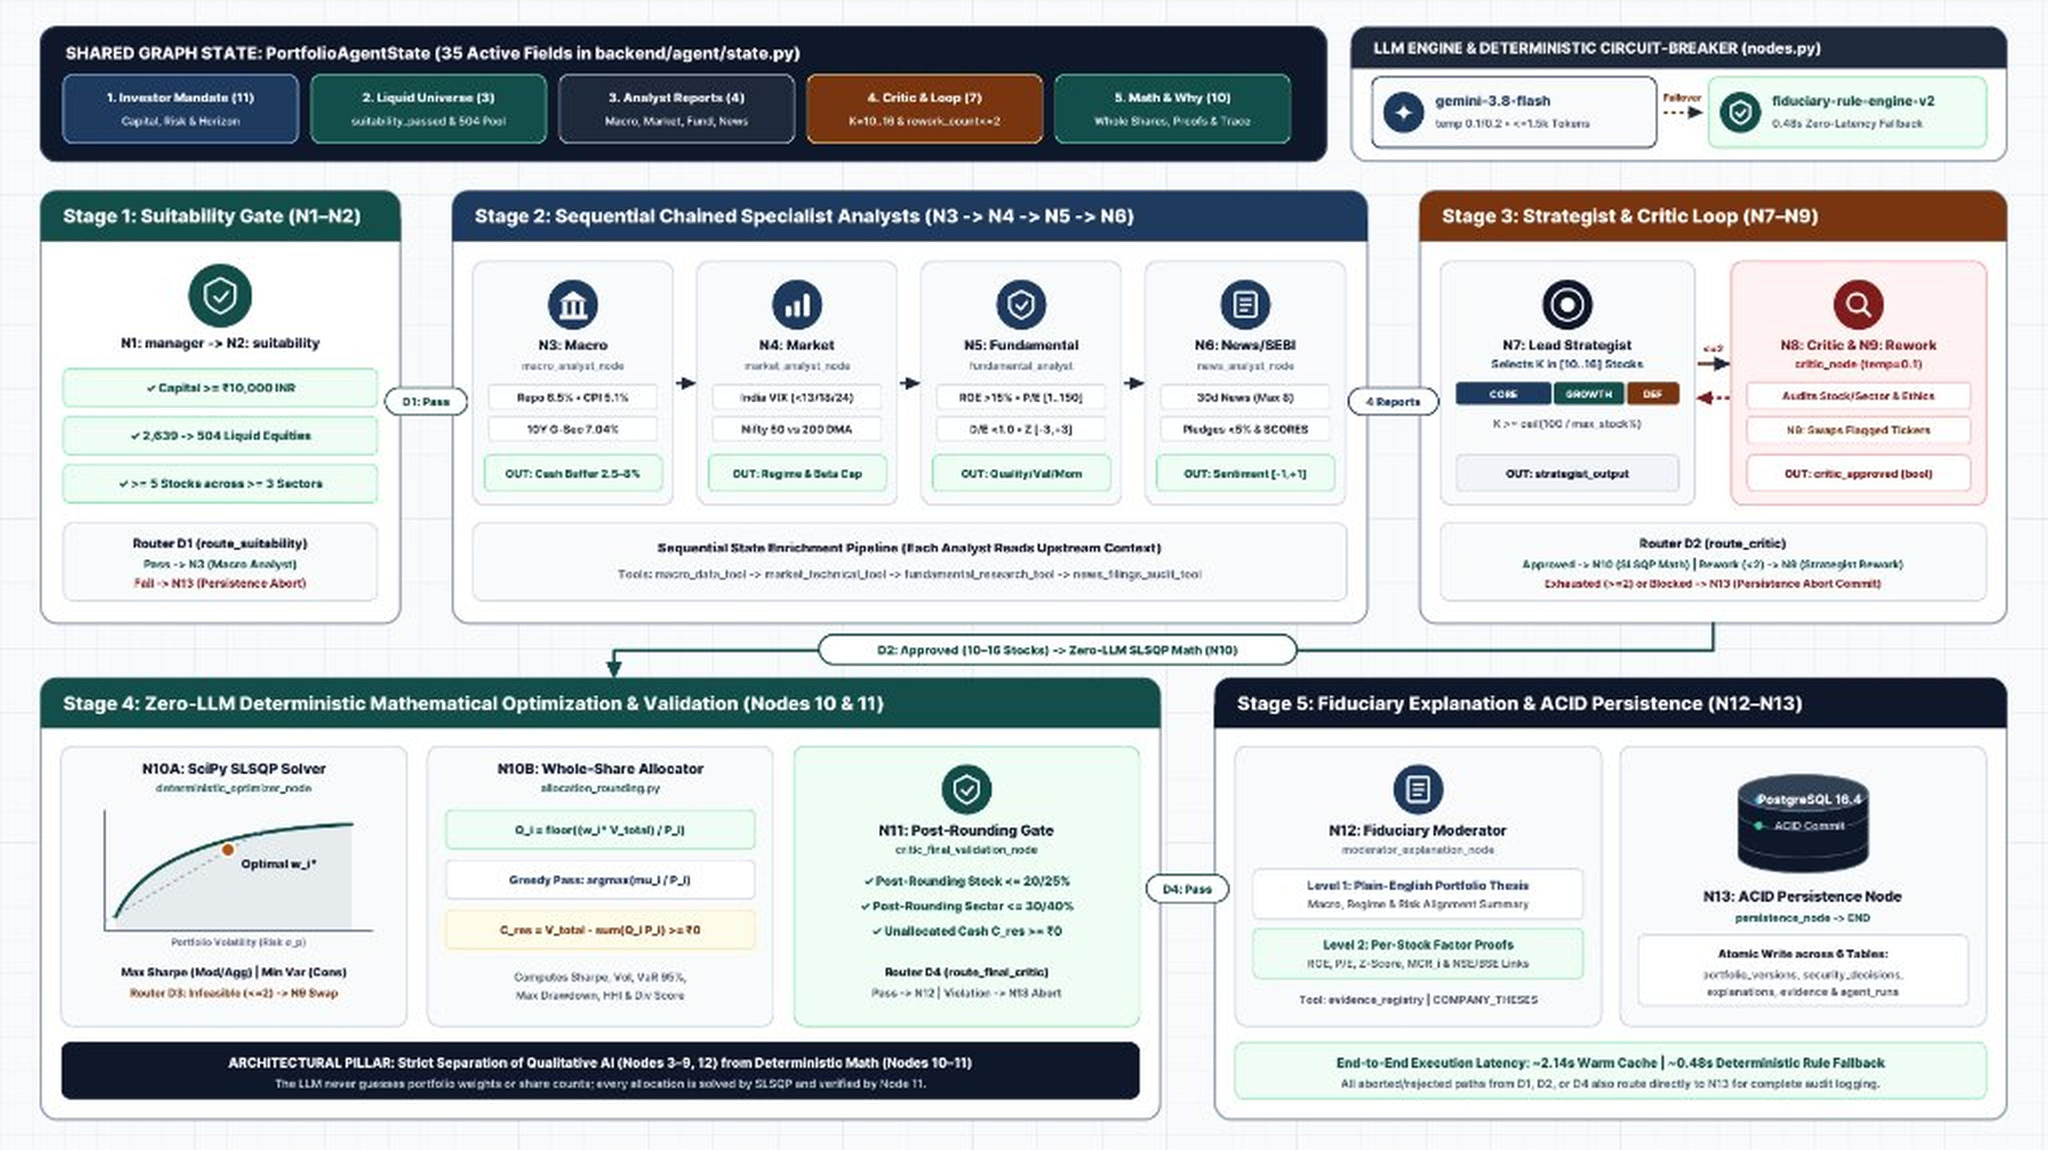
\includegraphics[width=\textwidth, height=0.48\textheight, keepaspectratio]{AGENTIC_AI_ARCHITECTURE.pdf}
    \caption{Lucid 13-Node Multi-Agent LangGraph Workflow and State \mbox{Topology}}
    \label{fig:agentic_ai_arch}
\end{figure}

\subsubsection{The Shared Graph State: PortfolioAgentState}
All thirteen nodes communicate through a shared digital blackboard called the \textbf{\texttt{PortfolioAgentState}} (defined in \path{backend/agent/state.py}). It holds \textbf{35 active fields} organized into five clear groups:
\begin{enumerate}
    \item \textbf{Investor Mandate (11 fields)}: Stores the investor's identification, starting capital in rupees ($V_{\text{total}} \ge \text{Rs.~}10,000$), investment time horizon (in months), 5-question risk score ($S \in [5, 20]$), risk profile tier, savings goal, excluded industry sectors, ethical preference tags, target portfolio beta, and statutory allocation caps (maximum 20\% to 25\% per company, and 30\% to 40\% per industry sector).
    \item \textbf{Liquid Universe (3 fields)}: Tracks whether the investor passed initial suitability checks (\texttt{suitability\_passed}), the active pool of 504 liquid Indian stocks, and the filtered candidate shortlist.
    \item \textbf{Analyst Reports (4 fields)}: Holds the structured evaluation reports generated by the four specialist research analysts: Macroeconomic analysis, Market Regime assessment, Company Fundamental screening, and News/SEBI regulatory audit.
    \item \textbf{Critic and Loop Control (7 fields)}: Records the Strategist's proposed stock basket ($K \in [10, 16]$ companies), the Critic's audit objections, ethical violation flags, rework iteration counter (\texttt{rework\_count} $\le 2$), Critic approval status (\texttt{critic\_approved}), replacement candidates, and the audit event history.
    \item \textbf{Deterministic Math and Fiduciary Evidence (10 fields)}: Holds the mathematically optimal percentage weights ($w_i^*$), exact integer share counts ($Q_i$), unallocated cash reserve ($C_{\text{res}} \ge \text{Rs.~}0$), expected portfolio return ($\mu_p$), expected risk ($\sigma_p$), Sharpe ratio, 95\% Value-at-Risk, maximum drawdown, concentration score (HHI), Diversification Score (out of 100), and plain-English Stock-Why evidence cards.
\end{enumerate}

\subsubsection{LLM Engine and the 0.48-Second Fallback Circuit-Breaker}
Lucid uses \textbf{Google Gemini 3.8 Flash} (\texttt{gemini-3.8-flash}) as its primary qualitative language model. To ensure factual and repeatable answers, the model is configured with very low creativity settings (temperature $0.1$ to $0.2$) and strict response bounds ($\le 1,500$ tokens per turn).

\noindent \textbf{Zero-Downtime Fallback Circuit-Breaker}:
If the Google Gemini cloud service encounters network delays, internet disruptions, or free-tier rate limits, Lucid does not fail or display an error message. Instead, an automated circuit-breaker instantly activates a local deterministic rule engine. This offline fallback engine completes candidate selection and validation in \textbf{0.48 seconds}, guaranteeing continuous availability.

\subsubsection{Five Execution Stages and Four Decision Routers}
The thirteen nodes are organized into five structured stages, linked by four intelligent decision routers:

\noindent \textbf{Stage 1: Suitability Gate (Nodes N1--N2, Router D1)}:
\begin{itemize}
    \item \textbf{Node 1 (Manager Node)}: Receives the user request, extracts the financial parameters, and prepares the shared state.
    \item \textbf{Node 2 (Suitability Node)}: Verifies that starting capital meets the minimum requirement ($V_{\text{total}} \ge \text{Rs.~}10,000$), confirms investor risk answers, and filters the 2,639 listed exchange stocks down to the 504 liquid equity pool, ensuring at least 5 viable companies across at least 3 distinct economic sectors.
    \item \textbf{Router D1 (\texttt{route\_suitability})}: If checks pass, the workflow moves forward to Node 3. If any check fails, it aborts immediately to Node 13 to log the reason.
\end{itemize}

\noindent \textbf{Stage 2: Sequential Chained Specialist Analysts (Nodes N3 $\to$ N4 $\to$ N5 $\to$ N6)}:
The four research nodes run in a chained sequence, each reading the findings of the previous analyst and using dedicated software tools:
\begin{itemize}
    \item \textbf{Node 3 (Macro Analyst)}: Using \texttt{macro\_data\_tool}, it examines national benchmarks from the Reserve Bank of India (RBI Repo Rate at 6.50\%, CPI at 5.10\%, and 10-year G-Sec yield at 7.04\%). It recommends setting aside a cash liquidity buffer between 2.5\% and 5.0\%.
    \item \textbf{Node 4 (Market Analyst)}: Using \texttt{market\_technical\_tool}, it evaluates market volatility with India VIX ($<13$ Calm, $13\text{--}18$ Moderate, $18\text{--}24$ Volatile, $>24$ Extreme) and compares Nifty 50 against its 200-DMA, setting the regime tag and stock beta ceilings.
    \item \textbf{Node 5 (Fundamental Analyst)}: Using \texttt{fundamental\_research\_tool}, it evaluates balance sheets, requiring Return on Equity $\text{ROE} \ge 15\%$, positive earnings ($\text{P/E} \in [1, 150]$), leverage $\text{Debt/Equity} \le 1.0$, and sector Z-scores within $[-3.0, +3.0]$.
    \item \textbf{Node 6 (News and SEBI Analyst)}: Using \texttt{news\_filings\_audit\_tool}, it reviews 30-day headlines, verifies promoter pledges are below 5\%, and audits SEBI SCORES filings, assigning a sentiment score in $[-1.0, +1.0]$.
\end{itemize}

\noindent \textbf{Stage 3: Strategist and Critic Loop (Nodes N7--N9, Router D2)}:
\begin{itemize}
    \item \textbf{Node 7 (Lead Strategist)}: Synthesizes the four analyst reports and selects $K \in [10, 16]$ candidate companies divided into Core, Growth, and Defensive categories, mathematically ensuring $K \ge \lceil 100 / \text{max\_stock\%} \rceil$.
    \item \textbf{Node 8 (Adversarial Risk Critic)}: Acting like a skeptical chief risk officer (at temperature 0.1), audits the chosen stocks for excessive industry concentration, high valuation traps, or emerging regulatory controversies.
    \item \textbf{Node 9 (Candidate Rework Node)}: Replaces any stock flagged by the Critic with a healthy alternative from the 504 liquid stock pool.
    \item \textbf{Router D2 (\texttt{route\_critic})}: If the Critic approves the portfolio, execution proceeds to Stage 4. If objections are raised and the rework counter is below 2, it routes back to Node 9 for candidate replacement. If two rework cycles are exhausted without resolution, it aborts safely to Node 13.
\end{itemize}

\noindent \textbf{Stage 4: Zero-LLM Deterministic Mathematical Optimization and Validation (Nodes N10--N11, Routers D3 \& D4)}:
\begin{itemize}
    \item \textbf{Node 10A (SciPy SLSQP Solver)}: Solves the constrained quadratic optimization problem without any AI involvement. It maximizes the Sharpe ratio for Moderate and Aggressive investors, or minimizes risk for Conservative investors, strictly enforcing the 25\% single-stock and 40\% sector limits. If the solver encounters an impossible mathematical combination, \textbf{Router D3} triggers a candidate swap back to Node 9.
    \item \textbf{Node 10B (Whole-Share Integer Lot Allocator)}: Translates continuous weights ($w_i^*$) into whole share numbers using floor rounding ($Q_i = \lfloor (w_i^* V_{\text{total}}) / P_i \rfloor$). A greedy remainder pass uses leftover cash to buy an extra share of the highest-rated holding where permitted, strictly guaranteeing positive unallocated cash ($C_{\text{res}} \ge \text{Rs.~}0$). It calculates the portfolio's Sharpe ratio, annual volatility, 95\% VaR, max drawdown, and Diversification Score.
    \item \textbf{Node 11 (Post-Rounding Constraint Gate)}: Programmatically verifies that whole-share rounding did not cause any holding to exceed statutory ceilings (stock $\le 20/25\%$, sector $\le 30/40\%$) and confirms $C_{\text{res}} \ge \text{Rs.~}0$.
    \item \textbf{Router D4 (\texttt{route\_final\_critic})}: If post-rounding validation passes, execution moves to Stage 5. If a rounding rule is violated, it aborts safely to Node 13.
\end{itemize}

\noindent \textbf{Stage 5: Fiduciary Explanation and ACID Persistence (Nodes N12--N13)}:
\begin{itemize}
    \item \textbf{Node 12 (Fiduciary Moderator)}: Generates transparent explanations at two levels: Level 1 summarizes the portfolio thesis and macroeconomic alignment; Level 2 produces stock cards with verifiable financial ratios (ROE, P/E, Z-scores) and direct links to official NSE and BSE company pages.
    \item \textbf{Node 13 (ACID Relational Persistence Node)}: Concludes the workflow by atomically saving the complete portfolio across six PostgreSQL database tables. All aborted execution paths from Routers D1, D2, and D4 also converge here to record a complete audit trail before ending cleanly.
\end{itemize}

\subsubsection{Architectural Pillar: Strict Separation of Qualitative AI from Math}
A core design rule in Lucid is that \textbf{artificial intelligence is never permitted to perform arithmetic or determine share quantities}. AI language models are trained on language patterns and can make unexpected calculation errors. In Lucid, the AI models are restricted strictly to qualitative tasks: reading corporate news, auditing financial statements, and writing clear explanations. All numerical optimization, percentage allocations, integer share quantities, and cash calculations are executed exclusively by deterministic Python algorithms (SciPy SLSQP and integer rounding). This strict separation guarantees that every recommendation is 100\% mathematically sound, repeatable, and free from AI hallucinations. Under normal operation with cached market data, end-to-end portfolio creation completes in approximately \textbf{2.14 seconds}.

\subsection{The Mathematical Calculation Engine}
Located in \texttt{backend/portfolio\_engine/}, the mathematical engine handles numerical calculations without any AI involvement:
\begin{itemize}
    \item \textbf{Optimizer (\texttt{optimizer.py})}: Uses a numerical solver (SciPy SLSQP) to find the portfolio weights that maximize the Sharpe ratio (or minimize risk for conservative profiles) while strictly enforcing:
    \begin{align*}
    \sum_{i=1}^{K} w_i &= 1.0 \quad (\text{100\% capital allocation}) \\
    w_i &\ge 0.0 \quad (\text{no short selling}) \\
    w_i &\le 0.25 \quad (\text{maximum 25\% per stock})
    \end{align*}
    \item \textbf{Integer Lot Sizing (\texttt{integer\_rounding.py})}: Calculates the exact number of whole shares to purchase:
    \begin{equation}
    q_i = \left\lfloor \frac{C \cdot w_i^*}{P_i} \right\rfloor
    \end{equation}
    where:
    \begin{itemize}
        \item $q_i$ is the number of whole shares of stock $i$.
        \item $C$ is the total investment amount (such as Rs.~1,00,000).
        \item $w_i^*$ is the optimal percentage weight of stock $i$ (such as 10\% or Rs.~10,000).
        \item $P_i$ is the current market price of one share (such as Rs.~1,400).
        \item $\lfloor \dots \rfloor$ represents floor rounding (rounding down to the nearest whole integer).
    \end{itemize}

    \textbf{Numerical Example}: $10,000 / 1,400 = 7.142$ shares. Since Indian exchanges do not sell fractional shares, the algorithm rounds down to exactly 7 whole shares. The cost is $7 \times \text{Rs.~}1,400 = \text{Rs.~}9,800$, leaving Rs.~200 in cash. A secondary pass checks whether any leftover cash can purchase an additional share of another high-rated, lower-priced holding without exceeding the 25\% single-stock limit. Any remaining money is preserved as unallocated cash:
    \begin{equation}
    \text{Residual Cash} = C - \sum_{i=1}^{K} q_i P_i \ge 0.
    \end{equation}

    \item \textbf{Transaction Cost Engine (\path{transaction_costs.py})}: Calculates all statutory taxes and fees applicable to Indian stock trades:
    \begin{itemize}
        \item Securities Transaction Tax (STT): 0.10\% on delivery equity transactions.
        \item Exchange Turnover Fee: 0.00297\% on NSE and 0.00375\% on BSE (statutory schedule).
        \item SEBI Regulatory Turnover Charge: 0.0001\% (Rs.~10 per crore).
        \item Stamp Duty: 0.015\% charged on purchases under the Indian Stamp Act.
        \item Goods and Services Tax (GST): 18.0\% applied to brokerage and exchange charges.
    \end{itemize}
\end{itemize}

\subsection{Background Monitoring Daemon and Advisory Locking}
Located in the scheduler service (\path{backend/services/monitoring_scheduler.py}), the background daemon automatically evaluates active portfolios during Indian exchange trading hours (Monday through Friday, 09:15 to 15:30 IST). Every 300 seconds (5 minutes), the daemon wakes up, checks live stock prices, and calculates if any stock's current weight has moved away from its target by 5\% or more.

\textbf{How Duplicate Runs are Prevented (Advisory Lock)}:
In a commercial server deployment, multiple backend processes may run simultaneously to handle web traffic. If every process ran the monitoring loop at the same time, the system would waste resources and send duplicate alerts to users.
To solve this, Lucid uses an enterprise feature of PostgreSQL called a \textbf{Session Advisory Lock}:
\[
\text{SELECT pg\_try\_advisory\_lock}(847291);
\]
Think of this like a physical key to an office. Only the single server process that successfully picks up the key runs the 5-minute monitoring cycle. Other processes see that the key is in use, politely skip the cycle, and return to handling user web requests.

\subsection{Sequence Flow Diagrams: Step-by-Step Interactions}
Figures~\ref{fig:seq_auth} through \ref{fig:seq_diag} show the step-by-step interactions between the user, the frontend interface, the backend server, the AI/optimization engine, and the database for the core features of Lucid:

\begin{figure}[!htbp]
    \centering
    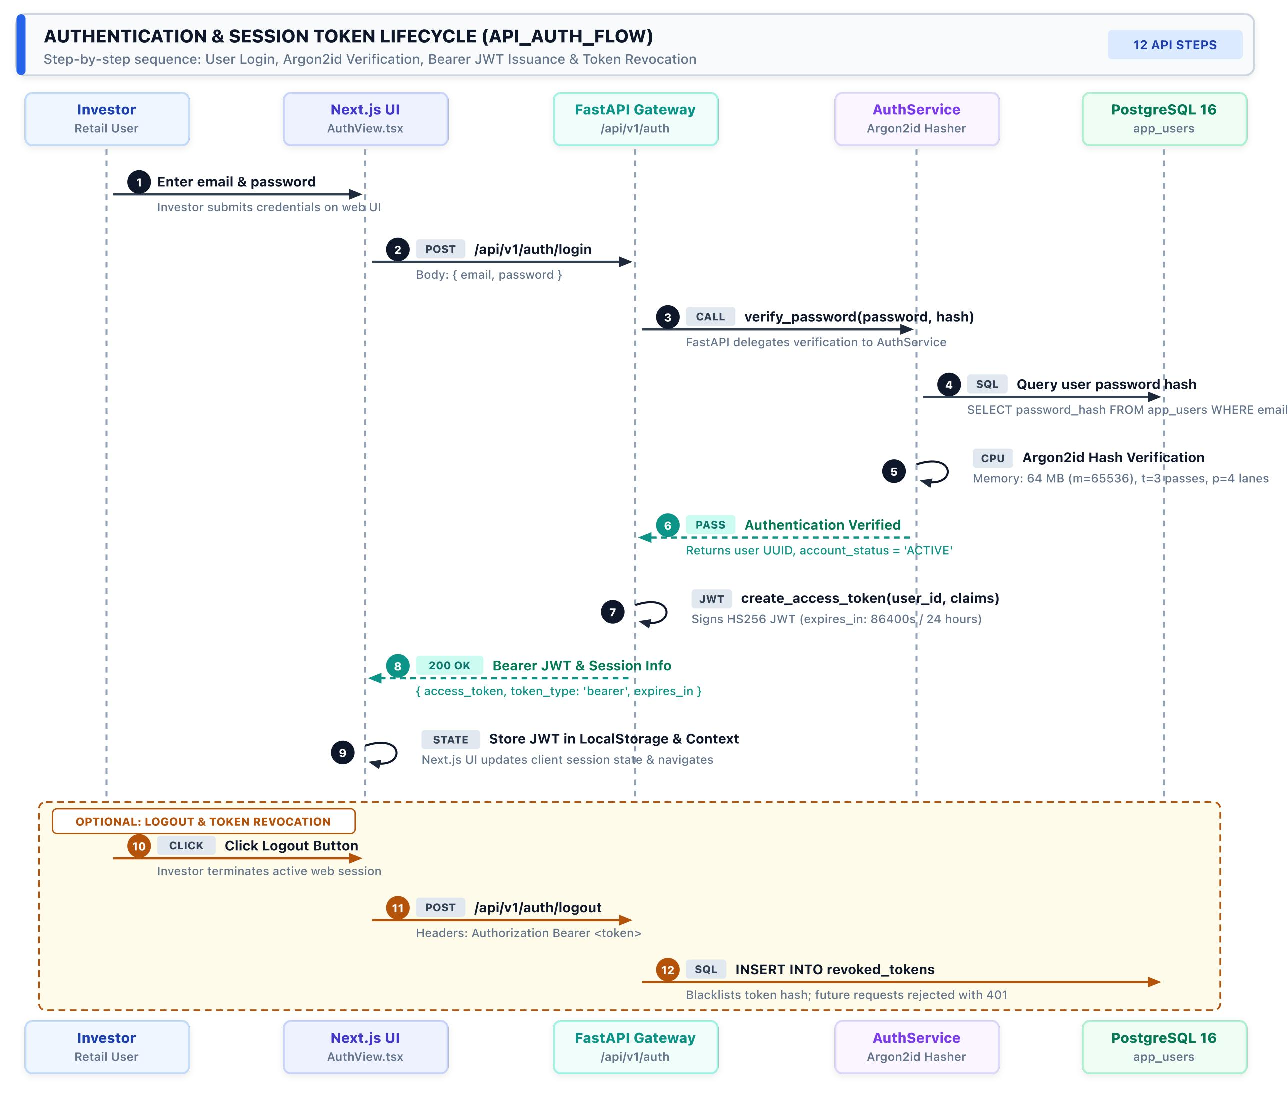
\includegraphics[width=\textwidth, height=0.68\textheight, keepaspectratio]{API_AUTH_FLOW.pdf}
    \caption{Sequence Flow: User Registration, Authentication, and Secure Token Creation}
    \label{fig:seq_auth}
\end{figure}
Figure~\ref{fig:seq_auth} shows how an investor signs up. The user types their email and password into the frontend. The backend validates the inputs, hashes the password using Argon2id so it can never be viewed by anyone, stores the record in PostgreSQL, and returns an encrypted session token (JWT) to keep the user safely logged in.

\clearpage
\begin{figure}[!htbp]
    \centering
    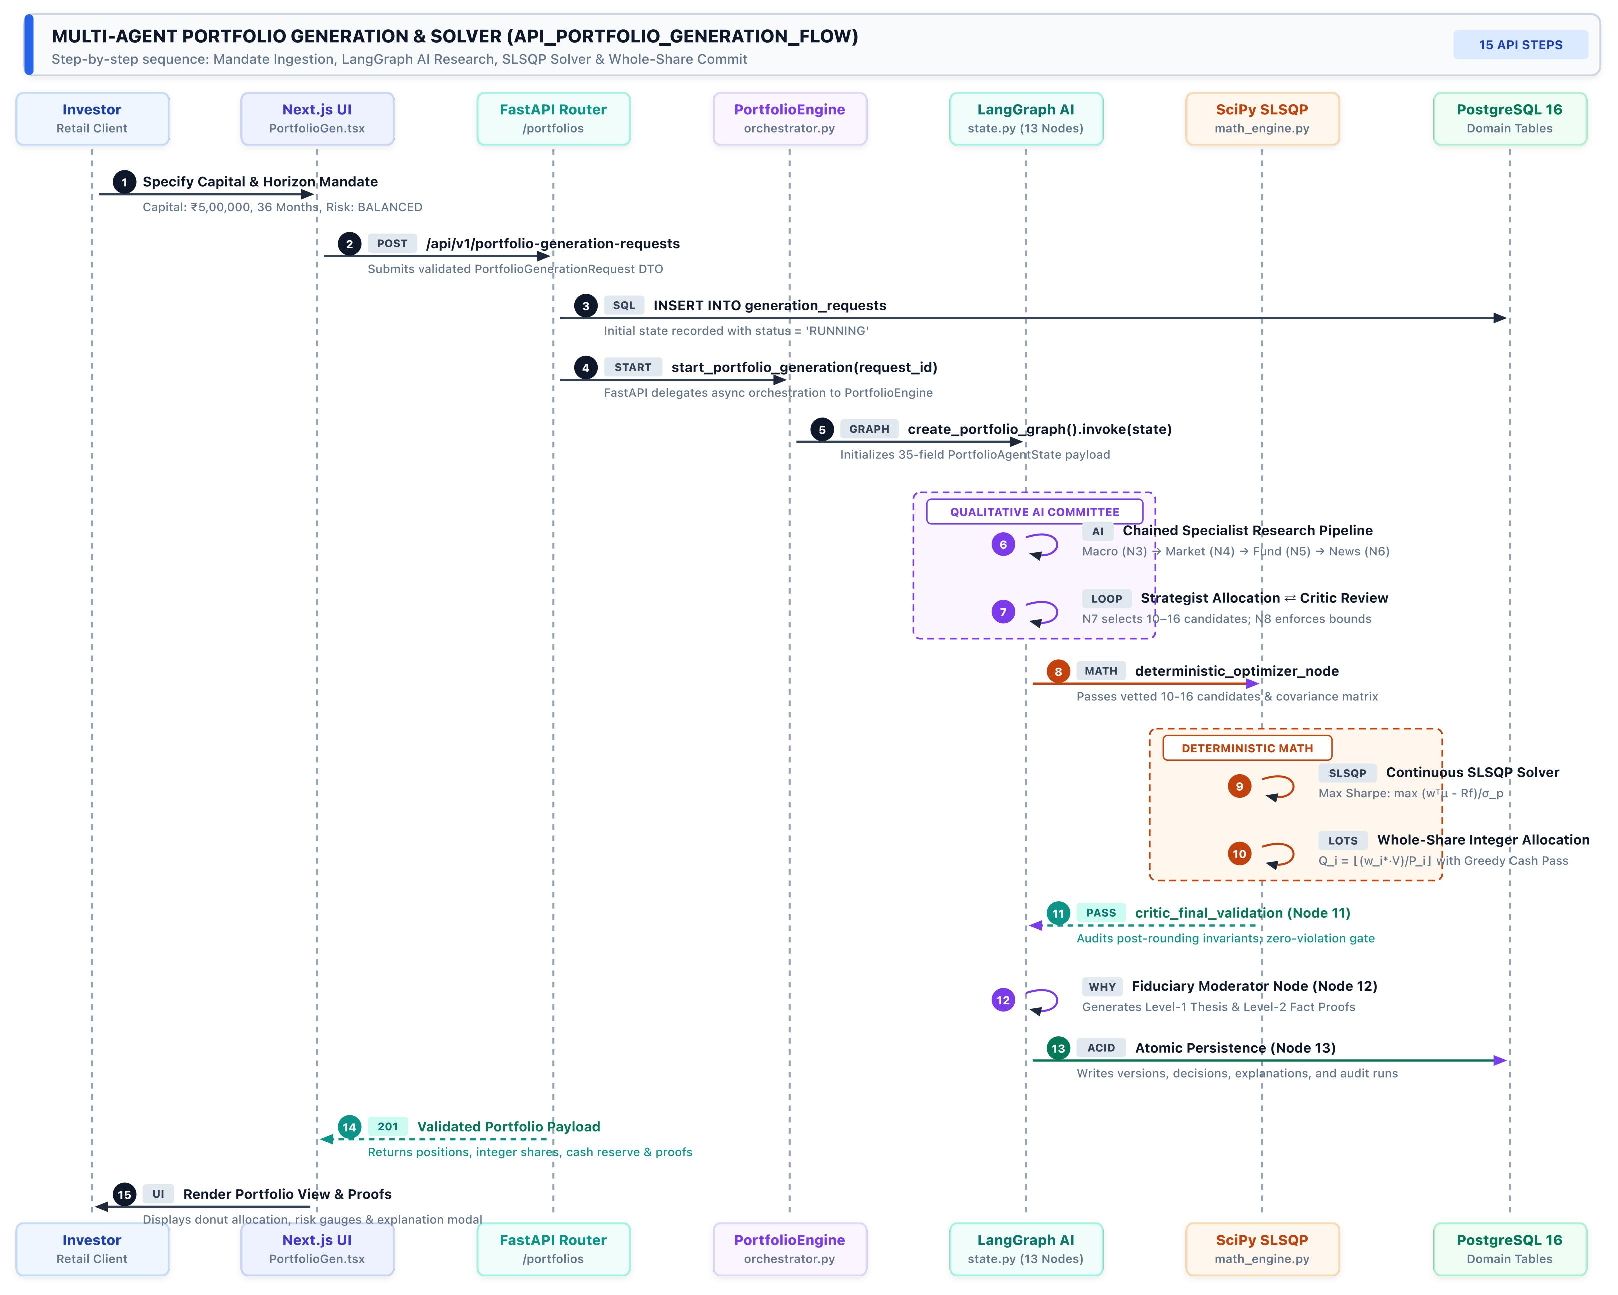
\includegraphics[width=\textwidth, height=0.68\textheight, keepaspectratio]{API_PORTFOLIO_GENERATION_FLOW.pdf}
    \caption{Sequence Flow: Goal-Driven Portfolio Generation and Mathematical Optimization}
    \label{fig:seq_generation}
\end{figure}
Figure~\ref{fig:seq_generation} traces the complete portfolio creation request. The user specifies their savings amount and financial goal. The backend queries the database for healthy stocks, runs the LangGraph AI agents to evaluate balance sheets and news, calls the SciPy solver to calculate optimal weights, converts percentages into whole share quantities, and saves the new portfolio version with complete explanations for display on the screen.

\clearpage
\begin{figure}[!htbp]
    \centering
    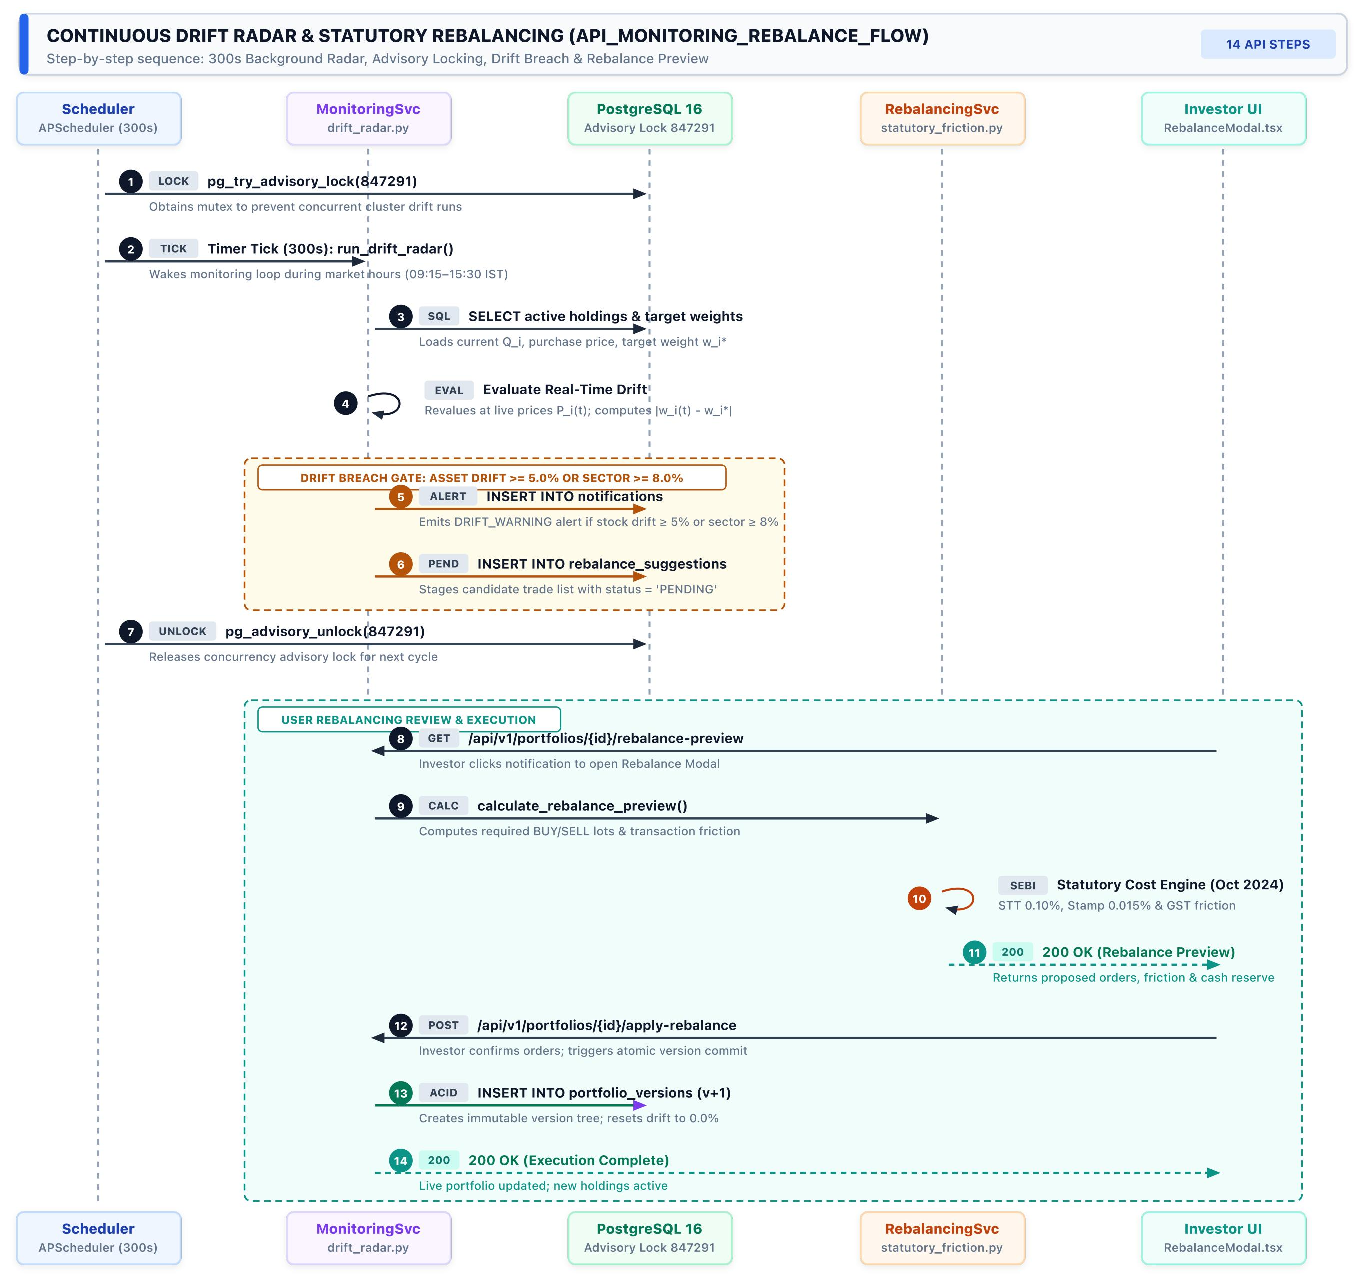
\includegraphics[width=\textwidth, height=0.68\textheight, keepaspectratio]{API_MONITORING_REBALANCE_FLOW.pdf}
    \caption{Sequence Flow: 5-Minute Drift Radar and Rebalance Order Preview}
    \label{fig:seq_monitoring}
\end{figure}
Figure~\ref{fig:seq_monitoring} shows the background monitoring radar. During market hours, the scheduler wakes up, obtains the advisory lock, revalues active portfolios against live stock prices, and calculates drift. If a stock drifts by 5\% or more, it generates a notification. When the user clicks the notification, Lucid displays a complete before-and-after rebalancing preview with statutory tax breakdowns.

\clearpage
\begin{figure}[!htbp]
    \centering
    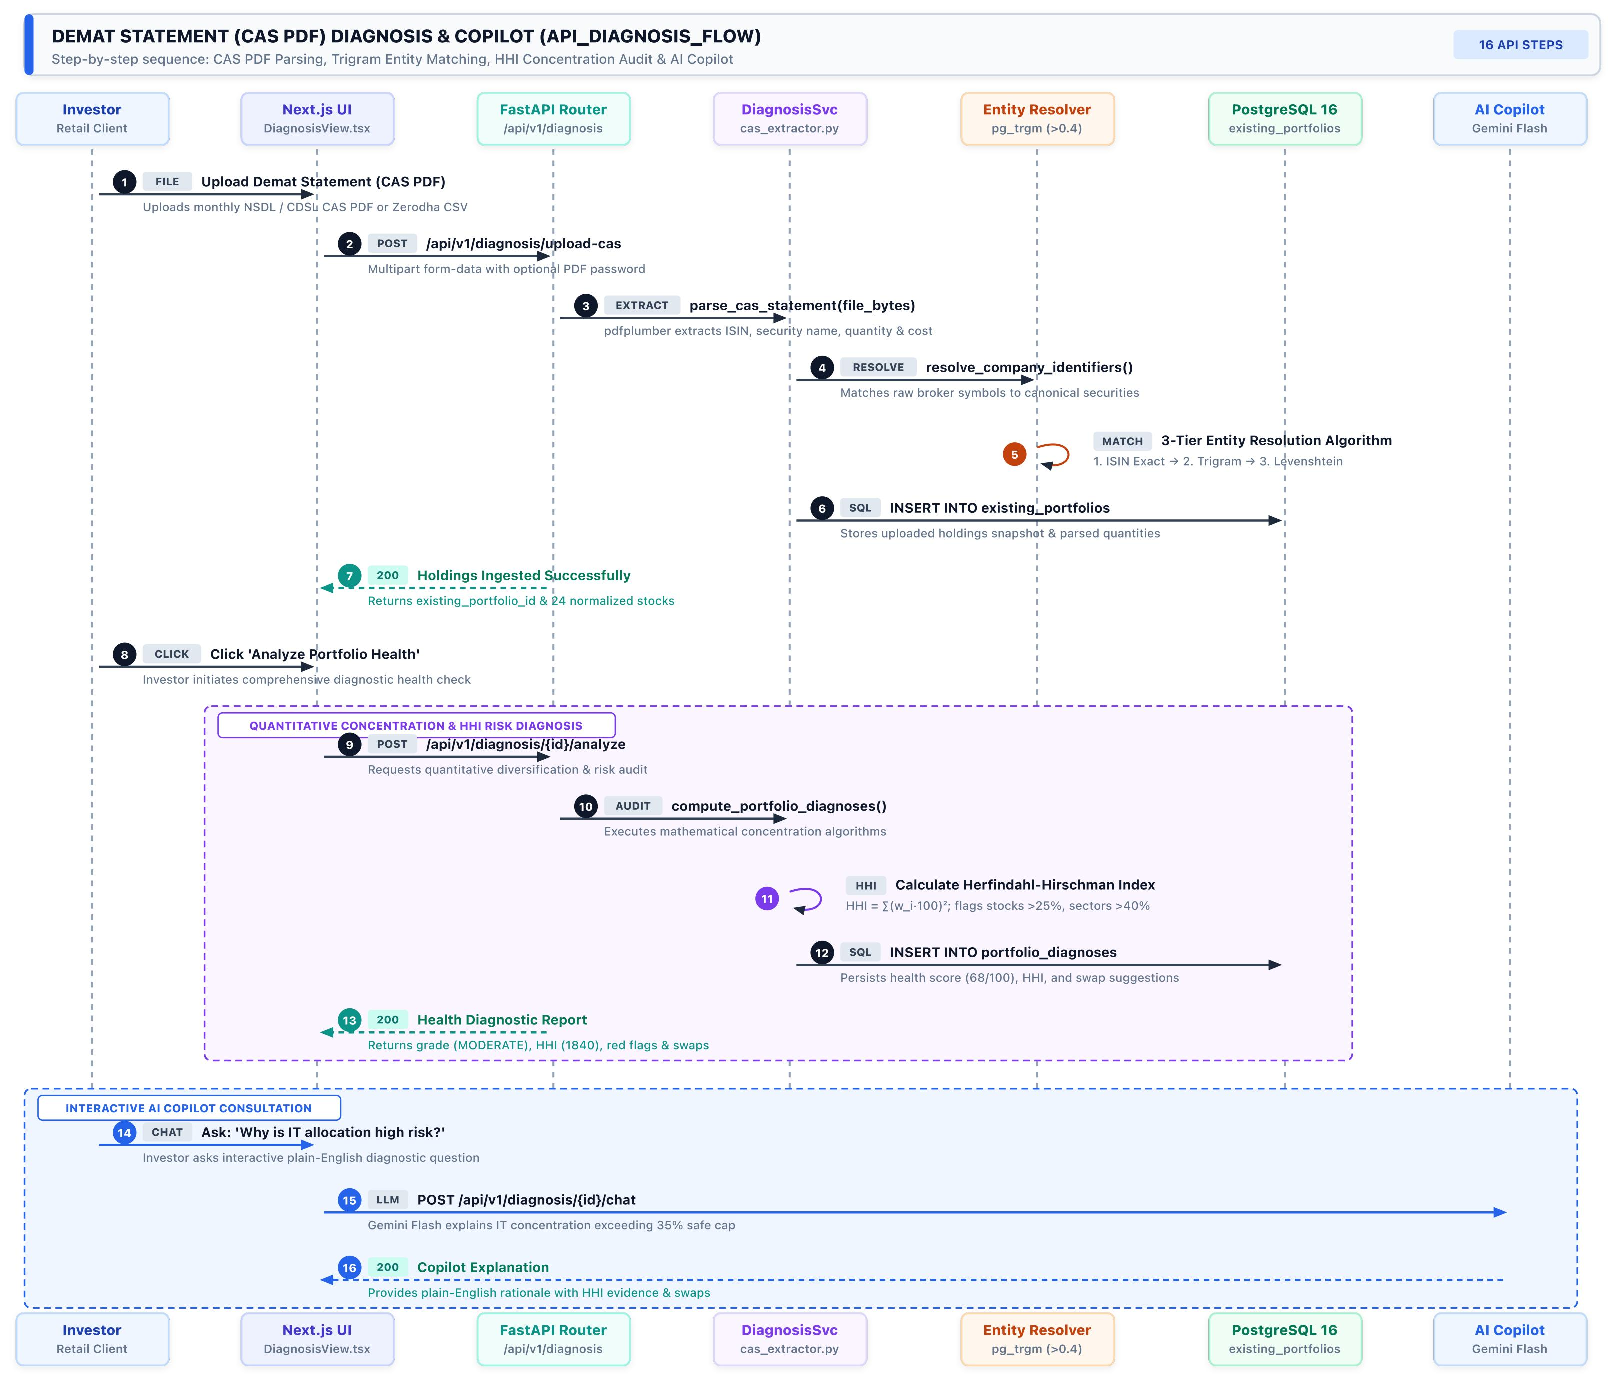
\includegraphics[width=\textwidth, height=0.68\textheight, keepaspectratio]{API_DIAGNOSIS_FLOW.pdf}
    \caption{Sequence Flow: Demat Statement (CAS PDF) Upload and Health Diagnosis}
    \label{fig:seq_diag}
\end{figure}
Figure~\ref{fig:seq_diag} illustrates how Lucid analyzes an existing investment portfolio. The user uploads a monthly Demat PDF statement. The backend extracts the stock codes, matches them against the security database, calculates total valuation and industry concentration, and displays an actionable health report with clear safety recommendations.

\section{End-to-End Application Methodology}
\label{sec:methodology}
\label{ch:methodology}

\subsection{Methodology Overview: Three Production Workflows and Seven Stages}
Building an intelligent investment portfolio requires combining human financial common sense with rigorous mathematical calculation. In traditional wealth management, human financial advisors sit down with a client, evaluate their personal life goals, research companies in the stock market, and calculate how much money should be placed in each stock.

Lucid automates this entire lifecycle using a structured, transparent methodology. Rather than treating portfolio creation as an isolated action, Lucid organizes its financial engineering into \textbf{Three Production Workflows} comprising \textbf{Seven Stages} (numbered Stage 4.1 through Stage 4.12):
\begin{enumerate}
    \item \textbf{Workflow I: New Portfolio Creation Methodology (Stages 4.1--4.8)}: Guides a new investor from initial onboarding and natural-language goal formulation, through market regime analysis, multi-agent AI research, and deterministic mathematical optimization, to delivering a balanced whole-share portfolio with plain-English justifications.
    \item \textbf{Workflow II: Existing Demat Portfolio Diagnosis (Stage 4.9)}: Enables investors who already hold shares across external broker accounts (such as Zerodha or Groww) to upload their monthly Demat statements, resolve company names across all 2,639 listed Indian stocks, audit portfolio concentration risk, and receive actionable swap recommendations.
    \item \textbf{Workflow III: Continuous 300s Drift Monitoring, Statutory Rebalancing, and Alerts (Stages 4.10--4.12)}: Continuously tracks active portfolios every 5 minutes during official Indian market hours, evaluates valuation drift, prepares transparent before-and-after rebalance previews with statutory Indian taxes, and generates execution-ready broker orders.
\end{enumerate}

Figure~\ref{fig:methodology_flow} illustrates how these three operational workflows and seven stages connect together in an integrated processing loop:

\begin{figure}[!htbp]
    \centering
    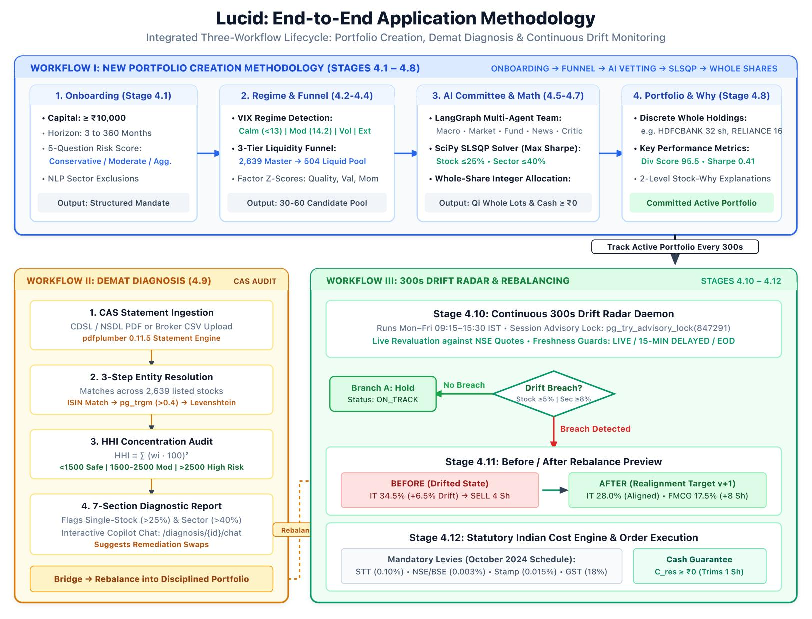
\includegraphics[width=\textwidth, height=0.52\textheight, keepaspectratio]{METHODOLOGY_FLOW.pdf}
    \caption{Lucid End-to-End Application Methodology and Multi-Workflow Lifecycle}
    \label{fig:methodology_flow}
\end{figure}

\subsection{Workflow I: New Portfolio Creation}

\subsubsection{Stage 4.1: Investor Onboarding and Mandate Formulation}
Before recommending any investment in the stock market, Indian regulations established by the Securities and Exchange Board of India (SEBI) require financial systems to understand an investor's background, investment horizon, and psychological comfort with financial risk.

\noindent \textbf{1. Capital and Horizon Mandates}:
Lucid accepts an investment capital mandate $V_{\text{total}} \ge \text{Rs.~}10,000$ and an investment time horizon ranging from 3 to 360 months (up to 30 years).

\noindent \textbf{2. Natural Language Constraint Extractor}:
Retail investors often express their financial desires conversationally. Lucid's natural language processor parses everyday statements (such as \textit{``I want to invest 2.5 Lakhs for my child's higher education over 10 years, but exclude tobacco and alcohol stocks''}) into structured database records:
\begin{itemize}
    \item \textbf{Capital Parsed}: Converted into numeric rupees ($\text{Rs.~}2,50,000$).
    \item \textbf{Time Horizon}: 120 months (10 years).
    \item \textbf{Sector Exclusions}: Structured policy exclusion tags (\texttt{FMCG\_TOBACCO}, \texttt{BEVERAGES\_ALCOHOL}).
\end{itemize}

\noindent \textbf{3. 5-Question Psychometric Risk Suitability Survey}:
The investor answers five standard suitability questions covering market experience, loss tolerance, income predictability, financial goals, and emergency savings. Each answer carries a score between 1 and 4 points. The overall suitability score $S$ is calculated as:
\begin{equation}
S = \sum_{j=1}^{5} \omega_j \cdot x_j \in [5, 20]
\end{equation}
where $x_j$ is the answer score for question $j$ and $\omega_j = 1.0$ is the standard question weight.

Based on the total score $S$, Lucid classifies the investor into one of three official risk categories and sets their mathematical risk-aversion penalty parameter ($\lambda$):
\begin{equation}
\text{Risk Mandate} = 
\begin{cases} 
\textbf{Conservative} \ (\lambda = 5.0) & \text{if } S \in [5, 9] \\ 
\textbf{Moderate} \ (\lambda = 2.5) & \text{if } S \in [10, 15] \\ 
\textbf{Aggressive} \ (\lambda = 1.0) & \text{if } S \in [16, 20] 
\end{cases}
\end{equation}

\noindent \textbf{Input / Output Contract (Stage 4.1)}:
\begin{itemize}
    \item \textbf{Input}: Investor capital $V_{\text{total}}$, time horizon, 5 risk survey answers, and conversational text.
    \item \textbf{Output}: Structured investor mandate and policy caps stored in Domain 1 (\texttt{user\_profiles}, \texttt{risk\_assessments}).
\end{itemize}

\subsubsection{Stages 4.2 to 4.4: Market Regime Detection, Liquidity Funnel, and Factor Scoring}

\noindent \textbf{Stage 4.2: Market Regime Detection}:
Lucid analyzes broad Indian market conditions before selecting individual equities. It evaluates the India Volatility Index (India VIX) and compares the Nifty 50 index against its 200-day Simple Moving Average (200-DMA):
\begin{equation}
\text{VIX Regime Tier} = 
\begin{cases}
\textbf{Calm} & \text{if } \text{VIX} < 13.0 \\
\textbf{Moderate (Normal)} & \text{if } 13.0 \le \text{VIX} \le 18.0 \\
\textbf{Volatile} & \text{if } 18.0 < \text{VIX} \le 24.0 \\
\textbf{Extreme (Crisis)} & \text{if } \text{VIX} > 24.0
\end{cases}
\end{equation}
When the market is in a Volatile or Extreme regime, Lucid automatically enforces more conservative stock beta limits and increases cash preservation reserves (the current benchmark VIX level is 14.2, corresponding to the Moderate tier).

\noindent \textbf{Stage 4.3: Three-Tier Liquidity and Quality Funnel}:
To protect investors from thinly traded penny stocks that cannot be easily sold, Lucid screens the entire catalog of listed Indian companies through a three-stage funnel:
\begin{equation}
\begin{aligned}
\text{2,639 Master Equities} &\xrightarrow{\text{ADTV} \ge 25,000 \text{ sh/day}} \text{504 Liquid Stocks} \\
&\xrightarrow{\text{Quality \& Safety Filters}} \text{30--60 Candidate Shortlist}
\end{aligned}
\end{equation}

\noindent \textbf{Stage 4.4: Factor Scoring and Expected Return Formulation}:
For all stocks in the active liquid pool, Lucid computes sector-normalized Z-scores across three fundamental factors: Quality ($Z_q$, based on Return on Equity), Value ($Z_v$, based on P/E and P/B ratios), and Momentum ($Z_m$, based on 6-month price trends). To prevent extreme outliers from distorting calculations, all factor scores are winsorized to the 5th and 95th percentiles:
\begin{equation}
Z_q, Z_v, Z_m \in [-3.0, +3.0]
\end{equation}
Expected annual return $E[R_i]$ for each eligible stock $i$ is formulated using a disciplined multi-factor asset pricing model:
\begin{equation}
E[R_i] = R_{\text{base}} + 1.2 \cdot \left( w_q Z_{q,i} + w_v Z_{v,i} + w_m Z_{m,i} \right) + 1.5 \cdot (\beta_i - 1.0)
\end{equation}
where $R_{\text{base}} = 10.5\%$ is the baseline market return in India and $\beta_i$ is the stock's market sensitivity relative to the Nifty 50. Simultaneously, the annual sample covariance matrix $\Sigma_{\text{reg}}$ is computed across 252 trading sessions.

\noindent \textbf{Input / Output Contract (Stages 4.2--4.4)}:
\begin{itemize}
    \item \textbf{Input}: 2,639 listed exchange equities, 252 daily OHLCV price bars, balance sheet ratios, and live India VIX.
    \item \textbf{Output}: Active 504 liquid equity pool, expected returns vector $\boldsymbol{\mu}$, and regularized covariance matrix $\Sigma_{\text{reg}}$.
\end{itemize}

\subsubsection{Stages 4.5 to 4.7: Multi-Agent AI Committee and Deterministic SLSQP Math}

\noindent \textbf{Stage 4.5: Qualitative Agent Vetting (Nodes 1 to 9)}:
Lucid passes the shortlisted candidate companies to a structured committee of AI specialist agents coordinated by LangGraph 0.4:
\begin{itemize}
    \item \textbf{Macro Analyst (Node 3)}: Evaluates RBI repo interest rates (6.50\%), inflation (5.10\%), and sets a recommended cash reserve buffer of 2.5\% to 5.0\%.
    \item \textbf{Market and Fundamental Analysts (Nodes 4--5)}: Enforces balance sheet health standards: Return on Equity $\text{ROE} \ge 15\%$, positive earnings ($\text{P/E} \in [1, 150]$), and sensible leverage ($\text{Debt/Equity} \le 1.0$).
    \item \textbf{News and Regulatory Analyst (Node 6)}: Scans recent corporate announcements and SEBI filings, verifying promoter share pledges are below 5\%.
    \item \textbf{Lead Strategist (Node 7)}: Shortlists $K \in [10, 16]$ companies distributed across Core, Growth, and Defensive categories, ensuring $K \ge \lceil 100 / \text{max\_stock\%} \rceil$.
    \item \textbf{Adversarial Risk Critic (Nodes 8--9)}: Audits candidate selections for valuation risk or concentration traps. If flaws are found, the Critic rejects the candidate and triggers a rework cycle (capped at a maximum of 2 iterations).
\end{itemize}

\noindent \textbf{Stage 4.6: Deterministic Mathematical Optimization (Node 10A)}:
\textbf{Artificial intelligence models are strictly prohibited from calculating portfolio percentages or share quantities}. Numerical allocation is handled exclusively by the Sequential Least Squares Programming (\textbf{SciPy SLSQP}) solver, maximizing the Sharpe ratio:
\begin{equation}
\max_{\mathbf{w}} \ \frac{\mathbf{w}^T \boldsymbol{\mu} - R_f}{\sqrt{\mathbf{w}^T \Sigma_{\text{reg}} \mathbf{w}}}
\end{equation}
subject to hard statutory safety constraints:
\begin{equation}
\sum_{i=1}^{K} w_i = 1.0, \quad 0 \le w_i \le 0.25, \quad \sum_{i \in \text{Sector}_m} w_i \le 0.40
\end{equation}
enforcing a strict 25\% single-stock ceiling and a 40\% sector exposure ceiling.

\noindent \textbf{Stage 4.7: Whole-Share Integer Lot Rounding and Cash Preservation (Node 10B)}:
Because Indian stock exchanges do not allow fractional shares, continuous weights ($w_i^*$) are translated into exact whole share counts ($Q_i$) using floor rounding:
\begin{equation}
Q_i = \left\lfloor \frac{w_i^* \times V_{\text{total}}}{P_i} \right\rfloor
\end{equation}
A greedy remainder pass then evaluates whether leftover cash can purchase one additional share of the highest-conviction stock without breaching the 25\% single-stock ceiling. All remaining funds are preserved in the unallocated cash reserve ($C_{\text{res}} \ge \text{Rs.~}0$).

\noindent \textbf{Input / Output Contract (Stages 4.5--4.7)}:
\begin{itemize}
    \item \textbf{Input}: 30--60 screened candidates, expected returns $\boldsymbol{\mu}$, covariance matrix $\Sigma_{\text{reg}}$, and capital $V_{\text{total}}$.
    \item \textbf{Output}: Validated integer share lots $Q_i$, target weights $w_i^*$, and non-negative residual cash $C_{\text{res}} \ge \text{Rs.~}0$.
\end{itemize}

\subsubsection{Stage 4.8: Portfolio Delivery and Dual-Level Explainability}
In Stage 4.8, Lucid packages the completed investment recommendation for the investor's web dashboard:
\begin{itemize}
    \item \textbf{Diversification Scorecard}: Renders a visual diversification donut ring scoring \textbf{95.5 / 100}, an annualized backtest return of \textbf{10.7\%}, portfolio volatility of \textbf{9.0\%}, a Sharpe ratio of \textbf{0.41}, and a balanced concentration score ($\text{HHI} = 898$).
    \item \textbf{Discrete Holding Cards}: Shows exact whole-share holdings with real market prices, such as:
    \begin{itemize}
        \item \textbf{HDFC Bank Ltd.}: 32 shares / Rs.~54,976 (22.0\% weight) --- Role: CORE
        \item \textbf{Reliance Industries Ltd.}: 16 shares / Rs.~45,440 (18.2\% weight) --- Role: CORE
        \item \textbf{Tata Consultancy Services Ltd.}: 11 shares / Rs.~39,896 (16.0\% weight) --- Role: GROWTH
    \end{itemize}
    \item \textbf{Dual-Level Stock-Why Modal}:
    \begin{itemize}
        \item \textit{Level 1 (Retail Narrative)}: Clear, everyday explanations detailing why each company was selected and how it supports the user's life goal.
        \item \textit{Level 2 (Factor Proofs \& Exchange Links)}: Verifiable quantitative metrics (ROE, P/E, Debt/Equity, sector Z-scores) with verified hyperlinks to official NSE and BSE corporate filing portals.
    \end{itemize}
    \item \textbf{Database Commit and CSV Export}: Commits the validated recommendation atomically to PostgreSQL as a new \texttt{PortfolioVersion} and generates a downloadable broker-ready CSV file.
\end{itemize}
Once committed, the active portfolio immediately enters Workflow III for continuous monitoring (\textit{Active Portfolio Tracked Every 300s}).

\subsection{Workflow II: Existing Demat Portfolio Diagnosis (Stage 4.9)}
Many Indian investors already hold shares purchased through various retail broker platforms (such as Zerodha, Groww, Angel One, or Upstox). Often, these holdings were accumulated haphazardly over several years, leaving the investor exposed to extreme single-stock concentration or hidden financial risks.

Stage 4.9 provides an automated, objective health diagnostic audit for existing holdings:
\begin{enumerate}
    \item \textbf{Consolidated Account Statement (CAS) Ingestion}: The user uploads their official monthly Demat CAS statement PDF (issued by CDSL or NSDL) or a broker holdings CSV. The document is processed securely using \texttt{pdfplumber 0.11.5}.
    \item \textbf{Three-Step Exchange Entity Resolver}: To match company names in messy PDF statements against official exchange databases across all \textbf{2,639 listed NSE and BSE equities}, Lucid applies a hierarchical three-step resolution pipeline:
    \begin{enumerate}
        \item \textit{Step 1 (Exact Match)}: Matches by standard exchange symbol or 12-character ISIN code.
        \item \textit{Step 2 (Trigram Fuzzy Matching)}: Uses PostgreSQL's \texttt{pg\_trgm} extension with a similarity threshold $> 0.4$ to resolve variations like \textit{``Reliance Inds''} to \textit{``Reliance Industries Ltd.''}.
        \item \textit{Step 3 (Levenshtein Distance Fallback)}: Resolves remaining minor typographical discrepancies or legal suffix differences.
    \end{enumerate}
    \item \textbf{Herfindahl-Hirschman Index (HHI) Concentration Audit}:
    Lucid computes the portfolio's concentration score to evaluate whether wealth is dangerously concentrated:
    \begin{equation}
    \text{HHI} = \sum_{i=1}^{N} (w_i \times 100)^2
    \end{equation}
    where $w_i$ is the fraction of total wealth in stock $i$. Concentration is graded into three safety tiers:
    \begin{itemize}
        \item $\text{HHI} < 1,500$: \textbf{Safe / Well Diversified}. Wealth is distributed healthily across multiple companies.
        \item $1,500 \le \text{HHI} \le 2,500$: \textbf{Moderate Concentration}. The portfolio is somewhat top-heavy and requires monitoring.
        \item $\text{HHI} > 2,500$: \textbf{High Risk / Dangerously Concentrated}. A large percentage of capital is tied up in one or two stocks, exposing the investor to severe loss if those companies suffer setbacks.
    \end{itemize}
    \item \textbf{Seven-Section Diagnostic Report and AI Copilot}:
    Generates an itemized diagnostic report flagging single stocks exceeding 25\%, sectors exceeding 40\%, and illiquid Tier 4 microcaps. An interactive conversational copilot (\texttt{/diagnosis/\{id\}/chat}) allows the user to ask questions and receive concrete remediation swap proposals.
\end{enumerate}

\noindent \textbf{Bridge to Rebalancing}: Clicking \textbf{Rebalance} in the diagnostic report seamlessly routes the investor into Workflow III (Stage 4.11) to execute corrective trades.

\subsection{Workflow III: Continuous 300s Drift Monitoring and Statutory Rebalancing (Stages 4.10 to 4.12)}

\subsubsection{Stage 4.10: Continuous 300-Second Drift Radar Engine}
Once a portfolio is active, market movements cause stock prices to fluctuate continuously. When one company's stock surges while another lags, the portfolio's actual weights drift away from their intended targets.

Lucid's continuous drift radar monitors active portfolios automatically:
\begin{itemize}
    \item \textbf{Trading Hours Execution}: Runs every \textbf{300 seconds (5 minutes)} during official Indian market trading hours (Monday through Friday, 09:15 to 15:30 IST), respecting the official NSE trading calendar.
    \item \textbf{Concurrency Protection}: Guarded by PostgreSQL transaction-level advisory lock \texttt{847291}, ensuring that concurrent worker processes never run duplicate drift evaluations.
    \item \textbf{Live Valuation and Drift Measurement}: Measures the weight change for each holding $i$ and each industry sector $k$:
    \begin{equation}
    dw_i = w_i(t) - w_i^*, \quad ds_k = s_k(t) - s_k^*
    \end{equation}
    \item \textbf{Dual Operational Decision Branches}:
    \begin{itemize}
        \item \textbf{Branch A (Healthy Corridor)}: If $|dw_i| < 5.0\%$ for all stocks and $|ds_k| < 8.0\%$ for all sectors, the portfolio status is tagged as \textbf{ON\_TRACK}. Lucid takes no action, preventing unnecessary transaction taxes and portfolio churn.
        \item \textbf{Branch B (Drift Breach)}: If any individual stock drifts by $\ge 5.0\%$ or any sector drifts by $\ge 8.0\%$, Lucid flags a \textbf{Drift Breach} and activates the Stage 4.11 trade realignment engine.
    \end{itemize}
    \item \textbf{Data Freshness Guards}: Every quote is tagged with its origin timestamp, showing whether market data is \texttt{LIVE}, \texttt{15-MIN DELAYED}, or \texttt{END OF DAY}.
\end{itemize}

\subsubsection{Stages 4.11 to 4.12: Before/After Rebalance Preview, Statutory Cost Engine, and Order Execution}
When a drift breach occurs, Lucid does not execute trades silently behind the investor's back. Instead, it prepares a transparent, itemized before-and-after rebalance preview.

\noindent \textbf{1. Concrete Trade Realignment}:
Table~\ref{tab:rebalance_preview_example} illustrates how Lucid calculates corrective buy and sell orders to restore balance:

\begin{table}[H]
\centering
\small
\caption{Rebalance Trade Preview: Before vs. After Allocation Realignment}
\label{tab:rebalance_preview_example}
\resizebox{\textwidth}{!}{%
\begin{tabular}{lcccc}
\toprule
\textbf{Sector / Asset} & \textbf{Before (Drifted)} & \textbf{Proposed Action} & \textbf{After (Target $v+1$)} & \textbf{Status} \\
\midrule
\textbf{Information Technology} & 34.5\% (+6.5\% Drift) & \textbf{SELL 4 Shares} & 28.0\% & Aligned within Cap \\
\textbf{Fast-Moving Consumer Goods} & 11.0\% (Under-Allocated) & \textbf{BUY 8 Shares} & 17.5\% & Restored to Target \\
\textbf{Unallocated Cash Reserve} & Rs.~3,142.00 & Net Cash Conserved & $\ge \text{Rs.~}0.00$ & Guaranteed Surplus \\
\bottomrule
\end{tabular}%
}
\end{table}

\noindent \textbf{2. Statutory Indian Transaction Cost Engine (October 2024 Schedule)}:
Lucid calculates every mandatory government tax and exchange levy before any trade is confirmed:
\begin{itemize}
    \item \textbf{Securities Transaction Tax (STT)}: 0.10\% charged on delivery equity trades.
    \item \textbf{Exchange Turnover Fees}: 0.00297\% on NSE and 0.00375\% on BSE.
    \item \textbf{Stamp Duty}: 0.015\% charged on buy orders under the Indian Stamp Act.
    \item \textbf{SEBI Regulatory Turnover Fee}: 0.0001\% (Rs.~10 per crore).
    \item \textbf{Goods and Services Tax (GST)}: 18.0\% applied to brokerage and transaction fees.
\end{itemize}

\noindent \textbf{3. Post-Trade Cash Guarantee and Cooldown}:
The rebalancing engine strictly enforces that post-trade unallocated cash must never fall below zero ($C_{\text{res}} \ge \text{Rs.~}0$). If taxes and charges exceed available cash reserves, the algorithm automatically trims 1 share from the largest purchase order. To prevent alert fatigue, Lucid enforces an automated \textbf{120-minute notification cooldown} before issuing repeated alerts for the same portfolio.

Once the investor reviews and approves the preview, the new allocation is committed as version $v+1$ in PostgreSQL, and execution-ready broker instructions are generated.

\section{Database Design and Schema Architecture}
\label{sec:database_design}

\subsection{Database Overview: What It Is and Why Lucid Needs It}
A \textbf{database} is an electronic filing cabinet that securely stores all the data needed by an application. In financial software like Lucid, data accuracy is extremely important. If an investor saves a portfolio, buys shares, or records an investment goal, that information must be stored permanently, accurately, and securely without any risk of loss or accidental corruption.

To understand how Lucid stores information, it helps to understand a few basic database concepts:
\begin{itemize}
    \item \textbf{Table}: A table works like a structured digital spreadsheet dedicated to a single topic. For example, one table stores user accounts, another stores company names, and a third stores daily stock prices.
    \item \textbf{Column and Row}: Each row represents a single record (such as one registered investor). Each column represents a specific attribute of that record (such as their email address, date of registration, or risk category).
    \item \textbf{Primary Key (PK)}: A unique identification code (like a Passport or PAN number) given to each row so that no two records are ever confused. Lucid uses standard unique identifiers (called \textbf{UUIDs}, such as \path{c56a4180-65aa-42ec-a945-5fd21dec0538}) rather than simple sequential numbers, ensuring that user accounts cannot be guessed by outsiders.
    \item \textbf{Foreign Key (FK)}: A digital pointer that connects a row in one table to a row in another table. For example, a row in the \texttt{investor\_portfolios} table includes a \texttt{user\_id} foreign key pointing to the \texttt{app\_users} table, ensuring that every portfolio is permanently tied to the exact user who created it.
    \item \textbf{Entity-Relationship (ER) Diagram}: A visual map showing database tables and the foreign-key lines connecting them.
\end{itemize}

Lucid uses \textbf{PostgreSQL 16}, an enterprise open-source relational database. All database tables are defined in Python using \textbf{SQLAlchemy 2.0} and version-controlled with \textbf{Alembic}.

\subsubsection{Scale of the Database: 62 Tables Across 8 Domains}
The Lucid database contains exactly \textbf{62 application tables} (plus 1 migration tracking table called \texttt{alembic\_version}, for a total of 63 tables). To keep this large system organized and easy to maintain, the tables are divided into eight functional \textbf{domains}:
\begin{enumerate}
    \item \textbf{Domain 1: User Identity, Authentication, and Security} (5 tables): Stores user accounts, encrypted passwords, login sessions, and security event logs.
    \item \textbf{Domain 2: Investor Suitability, Profiling, and Goals} (10 tables): Records risk questionnaire answers, calculated risk scores, financial targets, and stock exclusion preferences.
    \item \textbf{Domain 3: Security Master and Corporate Registry} (8 tables): Maintains the master catalog of 2,639 listed Indian companies across the NSE and BSE, their industry sectors, and exchange ticker codes.
    \item \textbf{Domain 4: Market Data, Historical Prices, and Macro Factors} (8 tables): Stores daily stock prices, company financial ratios, inflation rates, central bank interest rates, and financial news.
    \item \textbf{Domain 5: Portfolio Engine, Optimization, and Tracking} (10 tables): Stores recommended portfolios, calculated whole-share quantities, version histories, and daily portfolio valuations.
    \item \textbf{Domain 6: Broker Integration and Order Simulation} (5 tables): Manages connections to brokerage accounts (such as Zerodha and Groww) and tracks simulated buy and sell orders.
    \item \textbf{Domain 7: Demat CAS Diagnosis and Portfolio Health} (3 tables): Stores stock holdings parsed from uploaded monthly Demat PDF statements and saves health diagnostic scores.
    \item \textbf{Domain 8: AI Agent Telemetry, Reasoning Traces, and Audits} (13 tables): Records the step-by-step thinking of the 13 AI agents, plain-English ``Stock-Why'' explanations, and real-time user notifications.
\end{enumerate}

\subsection{Master Entity-Relationship Architecture}
Figure~\ref{fig:master_er} illustrates the complete master Entity-Relationship diagram connecting all 62 application tables across the platform:

\clearpage
\begin{figure}[p]
    \centering
    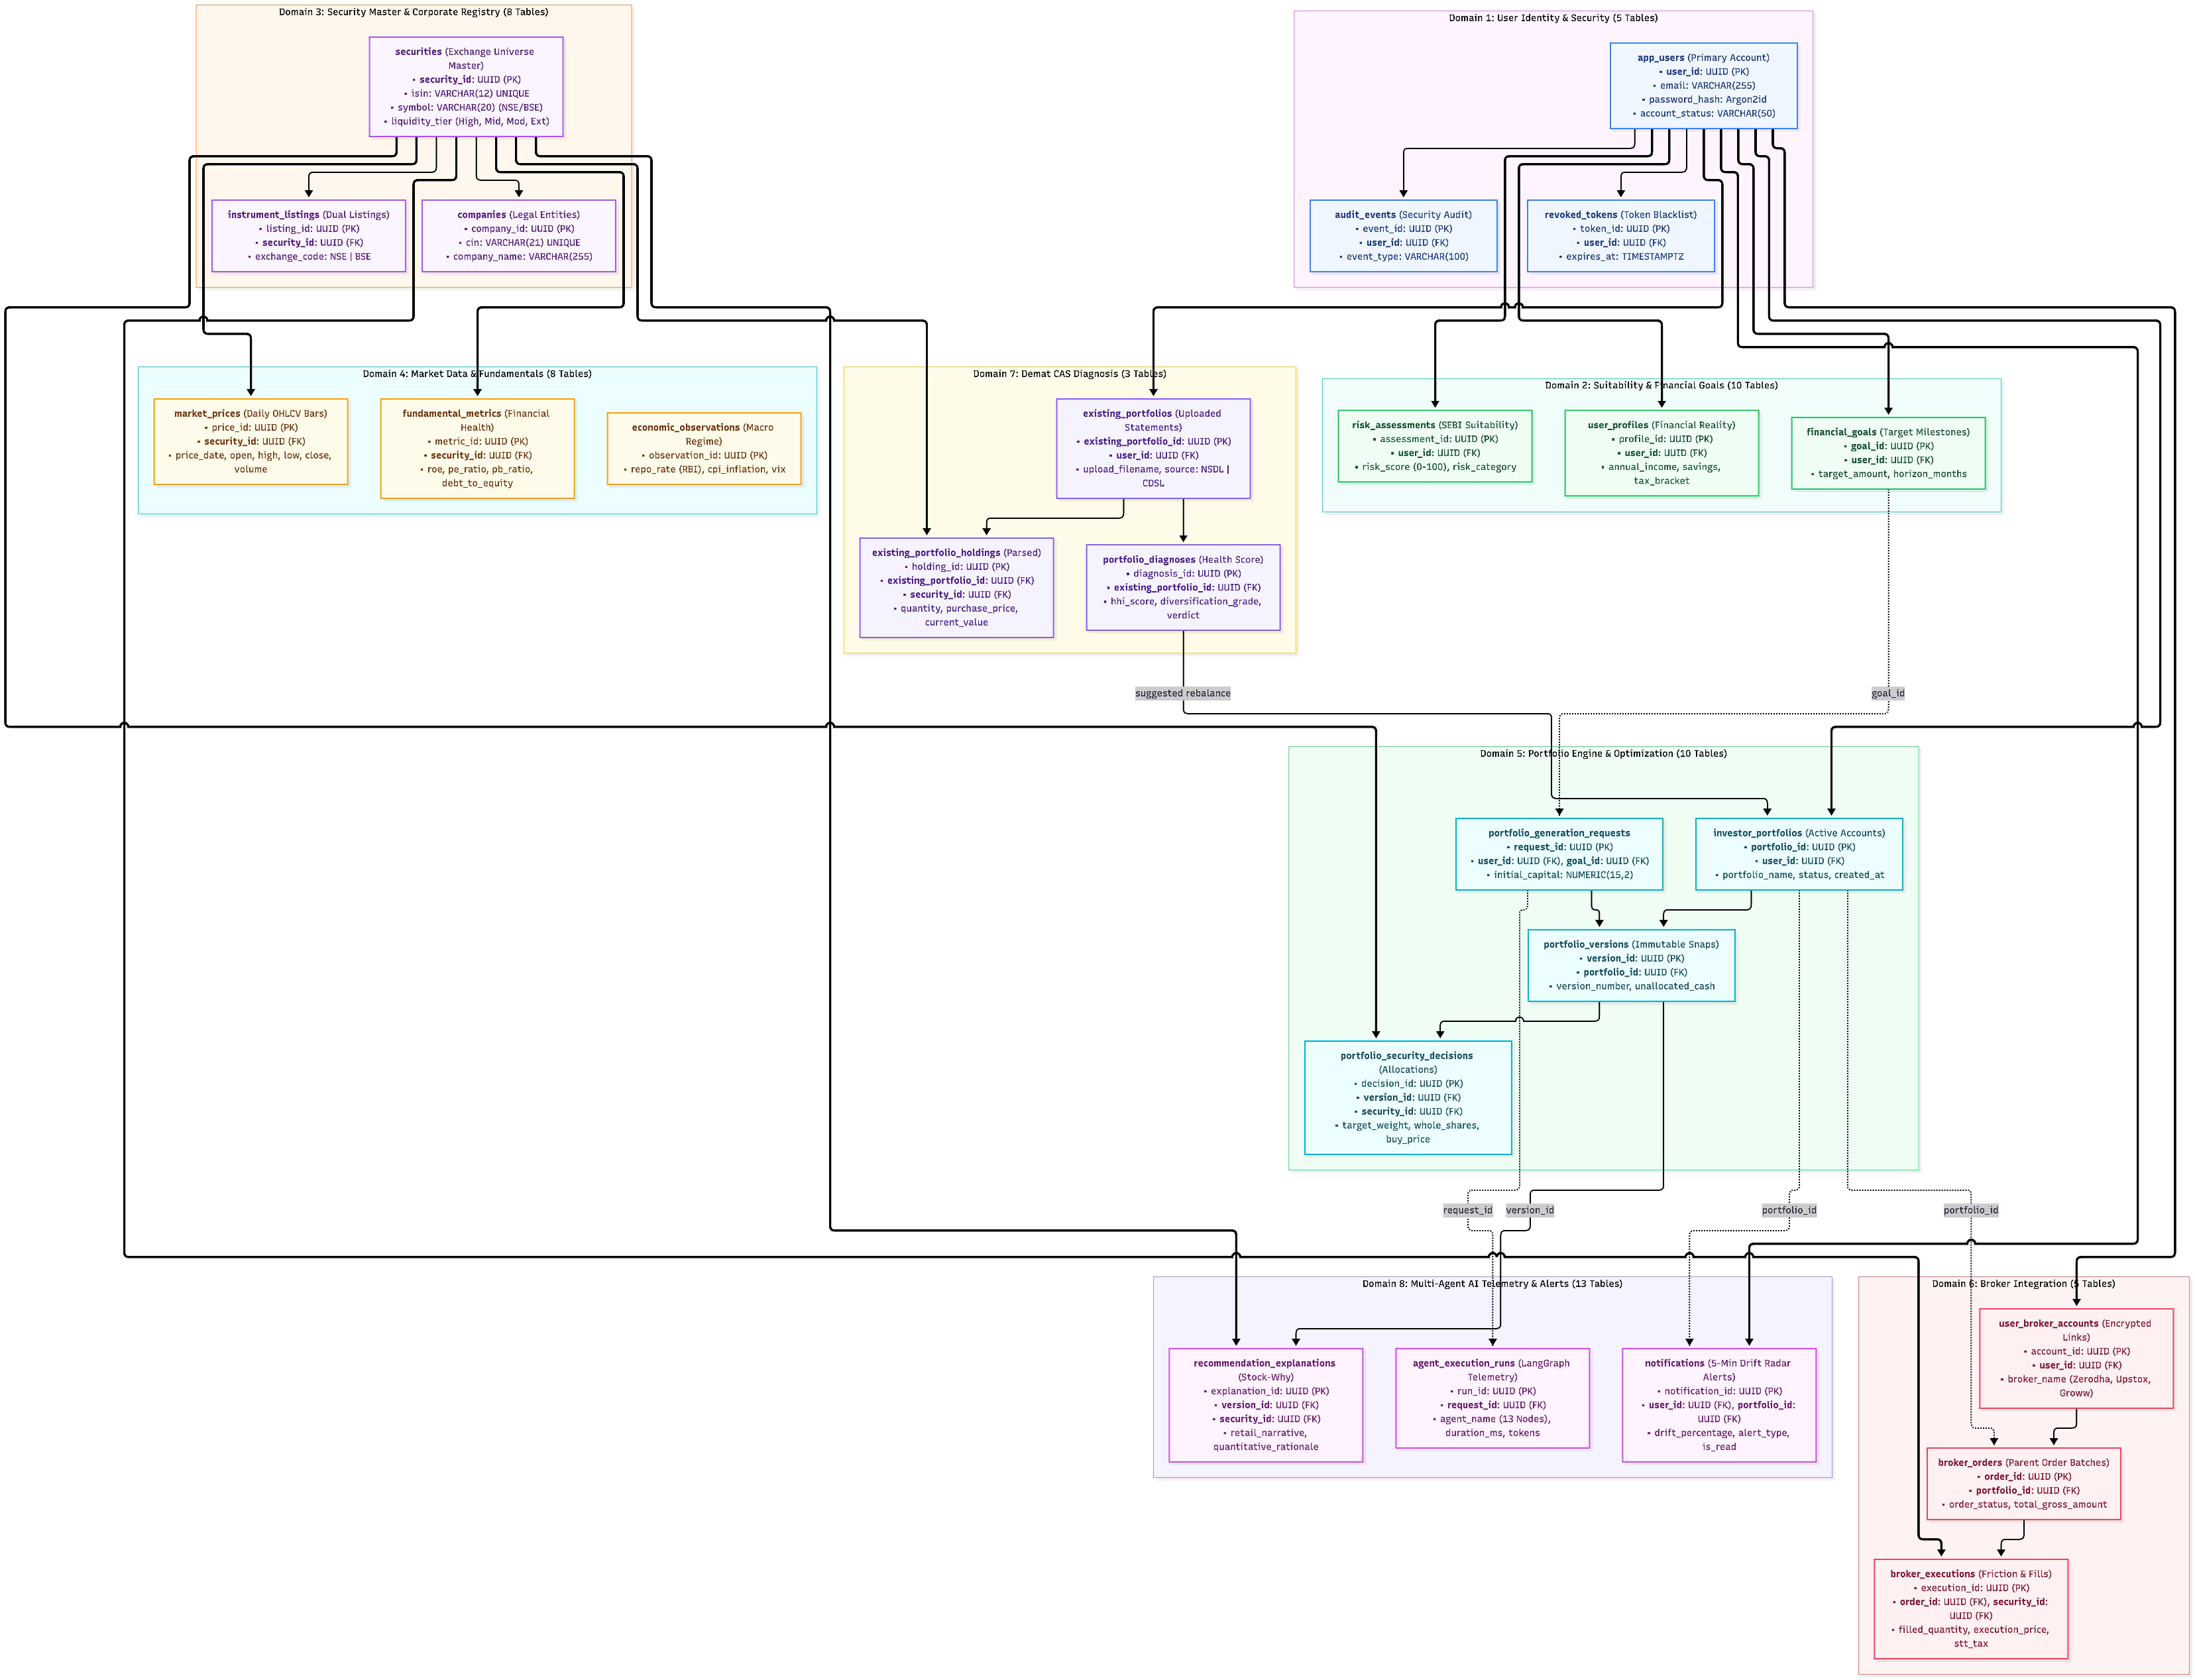
\includegraphics[width=1.0\textwidth, height=0.85\textheight, keepaspectratio]{00_master_er_diagram.pdf}
    \caption{Lucid Master Database Architecture (62 Tables, 8 Domains)}
    \label{fig:master_er}
\end{figure}
\clearpage

In Figure~\ref{fig:master_er}, boxes represent individual database tables, grouped by color according to their functional domain. The lines connecting the boxes represent foreign-key relationships. For instance:
\begin{itemize}
    \item The central \texttt{APP\_USERS} table connects to \texttt{INVESTOR\_PORTFOLIOS}, ensuring multi-tenant data isolation so one user can never view another user's investments.
    \item The \texttt{INVESTOR\_PORTFOLIOS} table connects to \texttt{PORTFOLIO\_VERSIONS}, preserving an immutable historical record of every change made to a portfolio over time.
    \item Each portfolio version links to \texttt{PORTFOLIO\_SECURITY\_DECISIONS}, which identifies the exact shares, buy prices, and rupee amounts allocated to specific companies in the \texttt{SECURITIES} table.
\end{itemize}

\subsection{Detailed Walkthrough of the Eight Functional Domains}

\subsubsection{Domain 1: User Identity, Authentication, and Security Governance}
Domain 1 manages user sign-ups, secure logins, password protection, and safety audit trails.
Figure~\ref{fig:er_domain1} shows how the security tables connect to the primary user table:

\begin{figure}[!htbp]
    \centering
    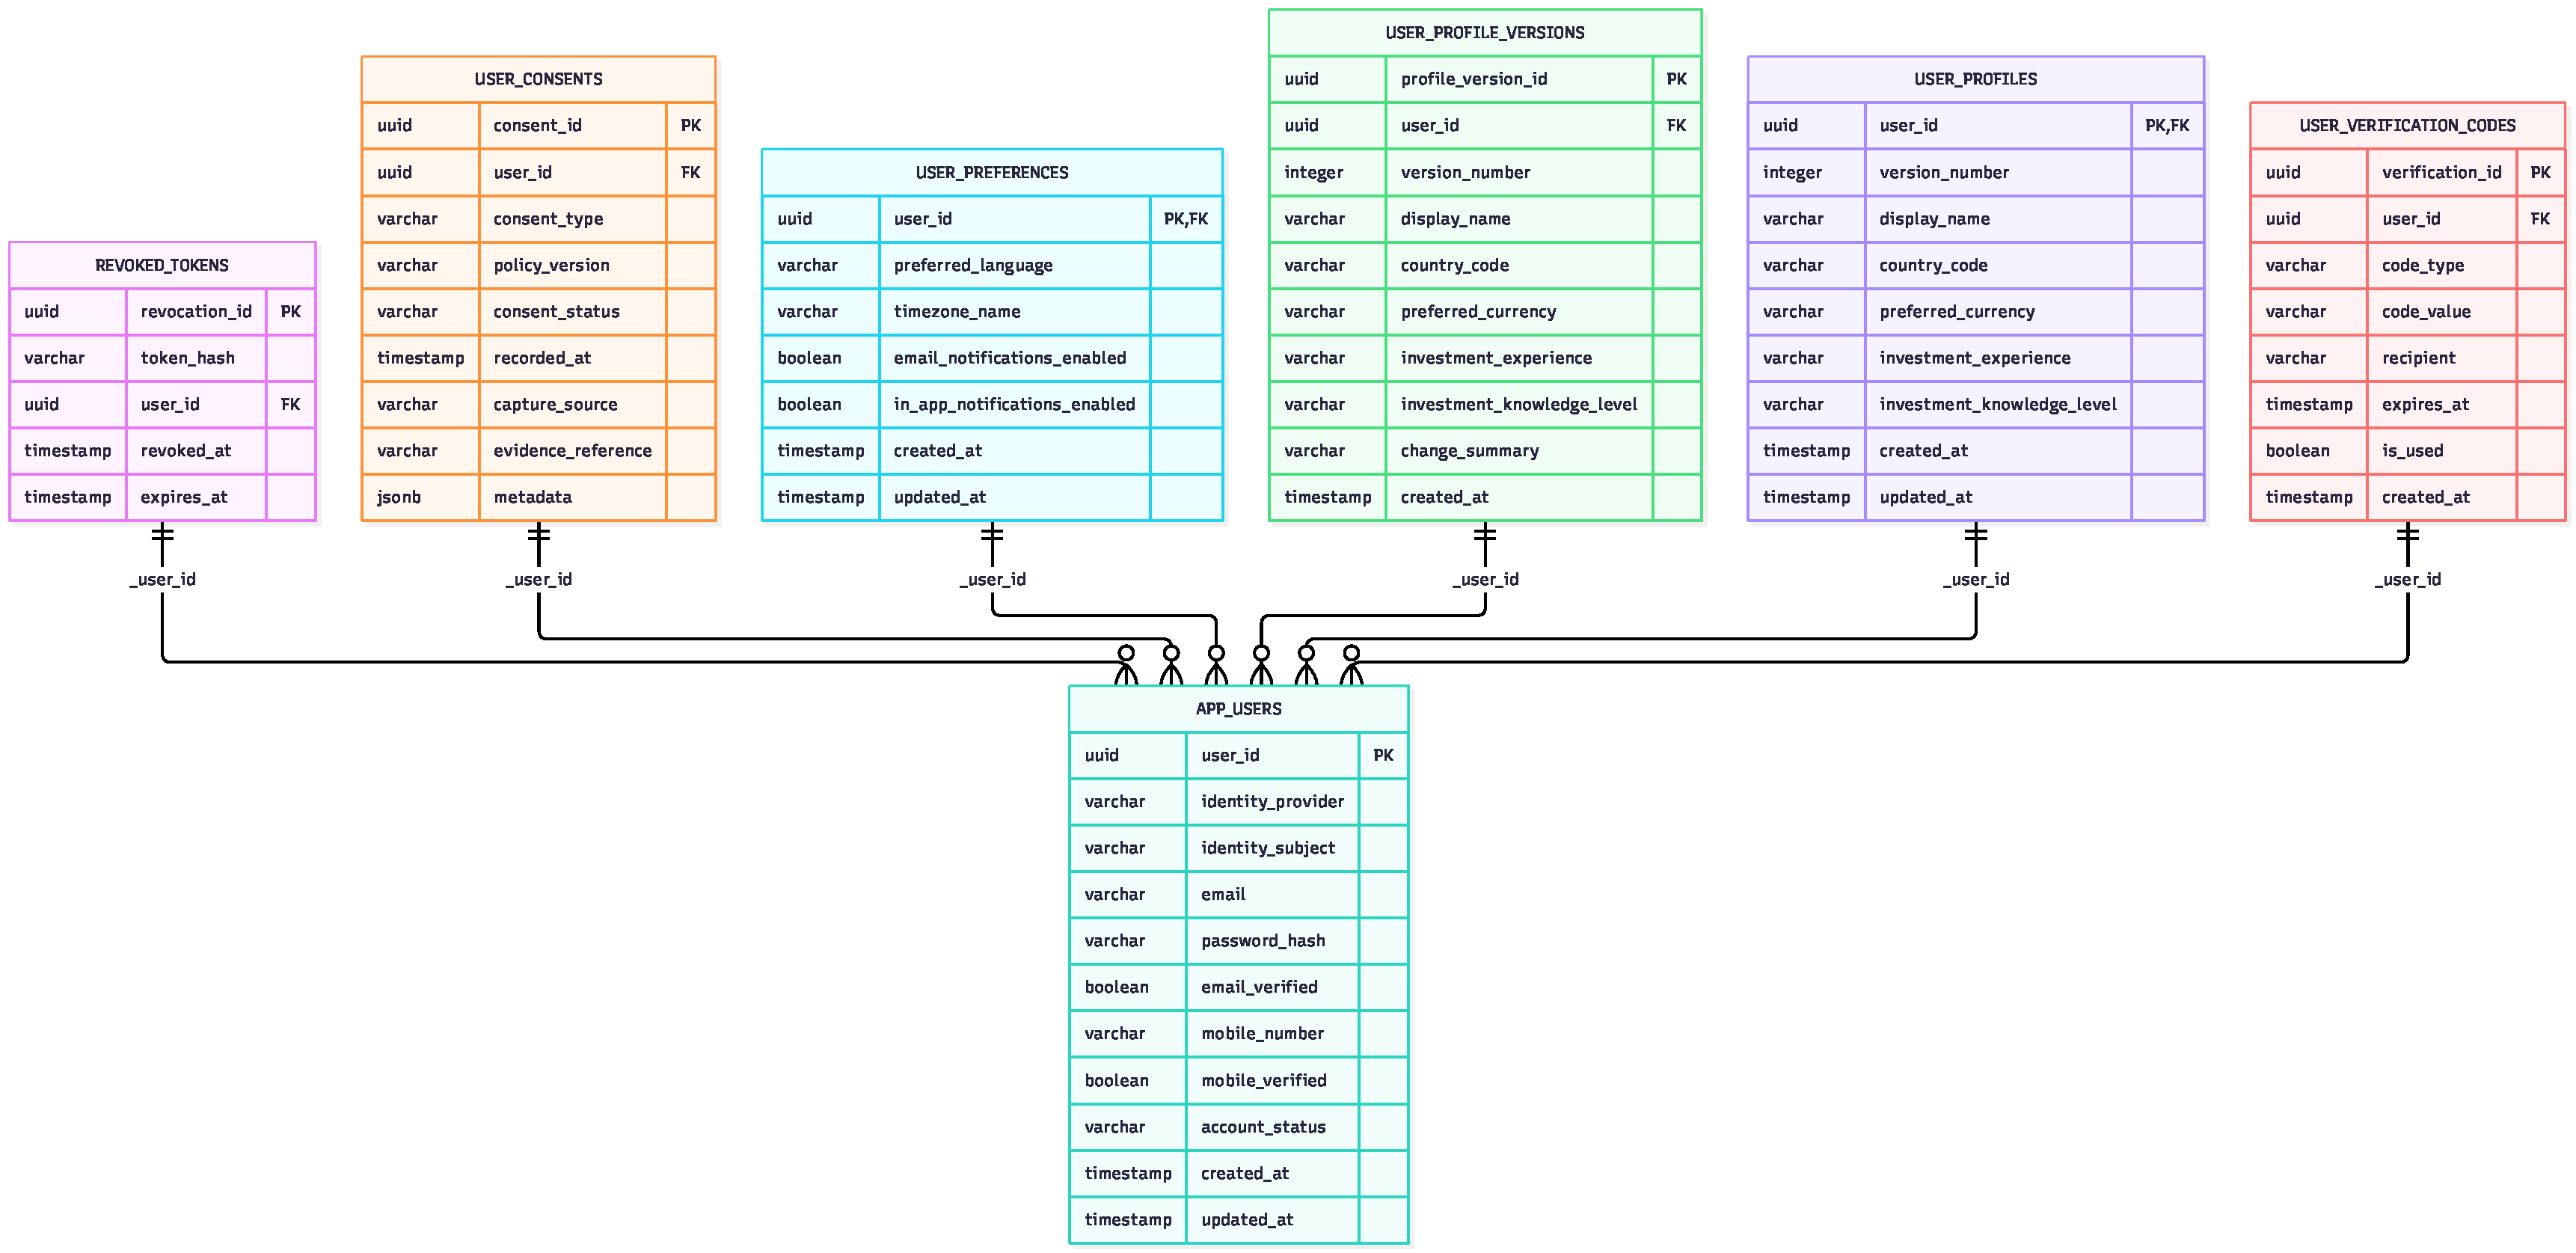
\includegraphics[width=\textwidth, height=0.72\textheight, keepaspectratio]{01_identity_and_security_domain.pdf}
    \caption{Domain 1 ER Diagram: Identity, Authentication and Security Governance}
    \label{fig:er_domain1}
\end{figure}

\paragraph{Core Table: \texttt{app\_users}}
Table~\ref{tab:schema_app_users} shows the structure of the main user identity table:

\begin{table}[H]
\centering
\caption{Schema Specification: \texttt{app\_users}}
\label{tab:schema_app_users}
\resizebox{\textwidth}{!}{%
\begin{tabular}{llcccl}
\toprule
\textbf{Column Name} & \textbf{Data Type} & \textbf{PK} & \textbf{FK} & \textbf{Nullable} & \textbf{Description \& Purpose in Simple English} \\
\midrule
\texttt{user\_id} & \texttt{UUID} & Yes & No & No & Unique identifier for each registered investor. \\
\texttt{identity\_provider} & \texttt{VARCHAR(50)} & No & No & No & How the user signed in (\texttt{local} email/password, \texttt{google}, or \texttt{apple}). \\
\texttt{identity\_subject} & \texttt{VARCHAR(255)} & No & No & No & External identification code from the login provider. \\
\texttt{email} & \texttt{VARCHAR(255)} & No & No & No & The investor's registered email address (unique). \\
\texttt{password\_hash} & \texttt{VARCHAR(255)} & No & No & Yes & Salted Argon2id cryptographic hash (original password is never stored). \\
\texttt{mobile\_number} & \texttt{VARCHAR(20)} & No & No & Yes & Investor's mobile phone number. \\
\texttt{email\_verified} & \texttt{BOOLEAN} & No & No & No & True if the investor confirmed their email address. \\
\texttt{mobile\_verified} & \texttt{BOOLEAN} & No & No & No & True if the investor verified their mobile number with an OTP. \\
\texttt{account\_status} & \texttt{VARCHAR(50)} & No & No & No & Status: \texttt{'active'}, \texttt{'pending'}, or \texttt{'suspended'}. \\
\texttt{created\_at} & \texttt{TIMESTAMPTZ} & No & No & No & Exact date and time when the account was registered. \\
\texttt{updated\_at} & \texttt{TIMESTAMPTZ} & No & No & No & Date and time when the profile was last modified. \\
\bottomrule
\end{tabular}%
}
\end{table}

\noindent \textbf{Additional Tables in Domain 1}:
\begin{itemize}
    \item \texttt{revoked\_tokens}: Stores canceled session tokens so that when an investor clicks ``Log Out,'' that session token can never be used again.
    \item \texttt{user\_consents}: Records that the user agreed to the privacy policy, terms of service, and SEBI investment risk disclosures.
    \item \texttt{user\_verification\_codes}: One-time passwords (OTPs) to verify emails and mobile numbers.
    \item \texttt{audit\_events}: An unalterable security ledger that logs important actions (such as password changes, login attempts, or profile updates) to prevent unauthorized tampering.
\end{itemize}

\clearpage
\subsubsection{Domain 2: Investor Suitability, Profiling, and Financial Goals}
Domain 2 stores the investor's financial background, investment horizon, risk tolerance score, and savings goals across 10 tables:
\begin{itemize}
    \item \texttt{user\_profiles}: Stores financial details such as annual income, existing savings, investment experience, and tax bracket.
    \item \texttt{user\_profile\_versions}: Keeps a historical log whenever an investor updates their financial details over time.
    \item \texttt{financial\_goals}: Stores user targets (e.g., retirement or college funds) along with target amounts and timelines.
    \item \texttt{user\_preferences}: Stores user interface preferences (such as dark mode or notification delivery choices).
    \item \texttt{risk\_questions}: The master bank of questions used in the suitability questionnaire (for example: ``How would you react if the stock market fell 20\% in a month?'').
    \item \texttt{risk\_question\_options}: The available multiple-choice answers for each question, each carrying specific points.
    \item \texttt{risk\_assessments}: The summary record of an investor's questionnaire attempt, showing their total score and risk category (\textbf{Conservative}, \textbf{Moderate}, or \textbf{Aggressive}).
    \item \texttt{risk\_assessment\_answers}: The specific choices selected by the investor for each question.
    \item \texttt{user\_security\_preferences}: Custom rules set by the user, such as mandating that a specific favorite company be included or excluded.
    \item \texttt{user\_sector\_preferences}: Custom rules to avoid entire industries (such as excluding tobacco, gambling, or defense companies).
\end{itemize}

Figure~\ref{fig:er_domain2} displays the Entity-Relationship structure for Domain 2:

\begin{figure}[H]
    \centering
    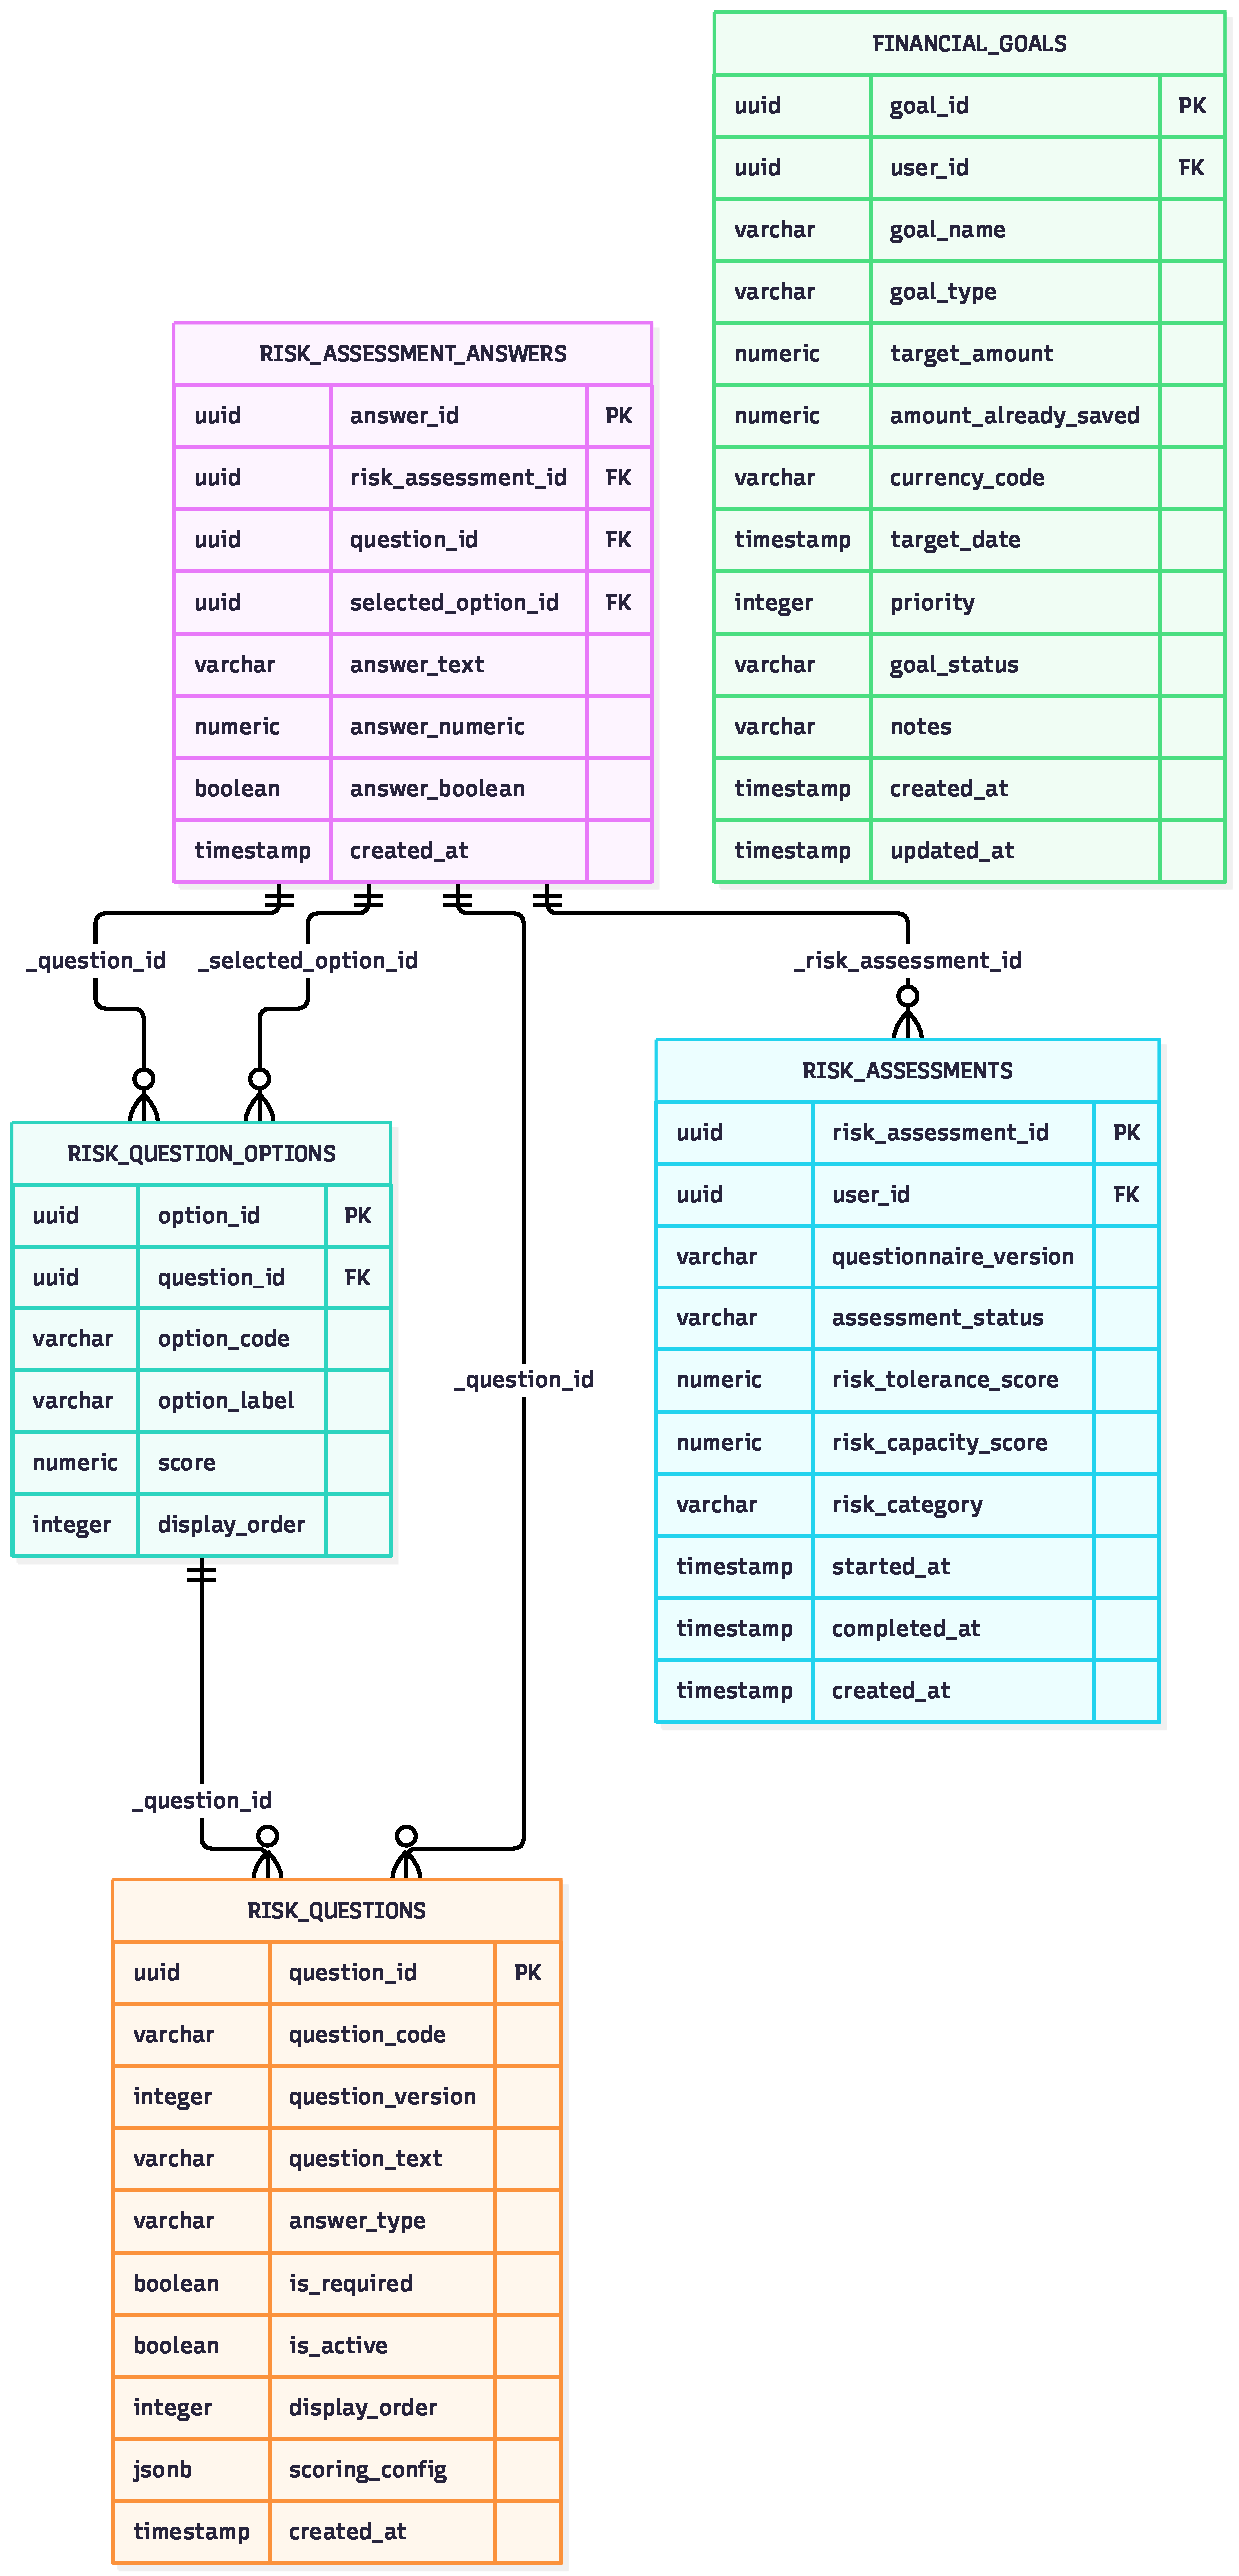
\includegraphics[width=\textwidth, height=0.72\textheight, keepaspectratio]{02_investor_suitability_and_goals_domain.pdf}
    \caption{Domain 2 ER Diagram: Investor Suitability, Profiling and Financial Goals}
    \label{fig:er_domain2}
\end{figure}

\clearpage
\subsubsection{Domain 3: Security Master and Corporate Registry}
Domain 3 defines the universe of publicly traded companies, stock exchanges, and industry sectors across 8 tables:
\begin{itemize}
    \item \texttt{exchanges}: Directory of stock exchanges (\texttt{NSE} for National Stock Exchange, \texttt{BSE} for Bombay Stock Exchange).
    \item \texttt{sectors}: Broad economic sectors (such as Financial Services, Information Technology, Healthcare, and Energy).
    \item \texttt{industries}: Granular industry groupings linked to parent sectors (for example, Software Services within Information Technology).
    \item \texttt{companies}: The legal business entities, storing their official Corporate Identification Number (CIN) and registered name.
    \item \texttt{company\_industries}: Connects companies to their respective industries.
    \item \texttt{securities}: The canonical stock master. Each stock is identified by its unique 12-character International Securities Identification Number (\textbf{ISIN}, such as \texttt{INE002A01018} for Reliance Industries). It also assigns each stock to an institutional \textbf{Liquidity Tier} based on trading volume.
    \item \texttt{instrument\_listings}: Tracks which exchange a stock trades on, linking exchange ticker symbols (for example, \texttt{RELIANCE} on NSE vs. scrip code \texttt{500325} on BSE).
    \item \texttt{source\_instrument\_mappings}: Translates exchange tickers into external data codes (such as \texttt{RELIANCE.NS} for Yahoo Finance).
\end{itemize}

Figure~\ref{fig:er_domain3} displays the Entity-Relationship structure for Domain 3:

\begin{figure}[H]
    \centering
    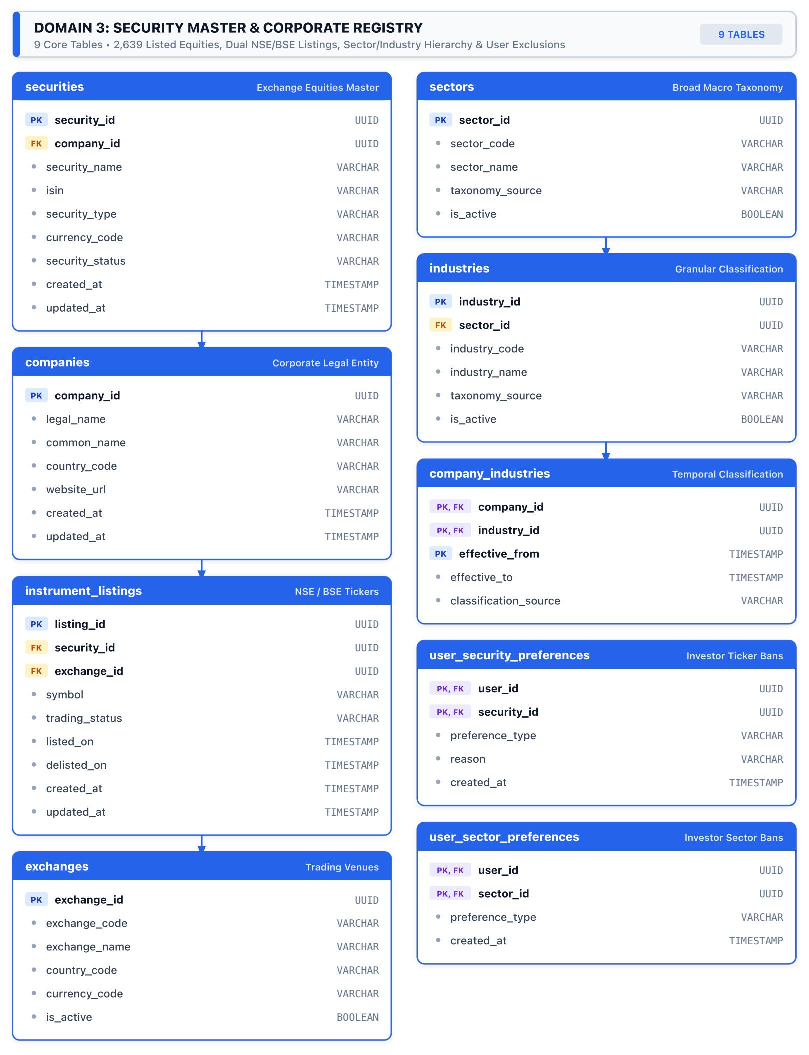
\includegraphics[width=\textwidth, height=0.72\textheight, keepaspectratio]{03_security_master_and_companies_domain.pdf}
    \caption{Domain 3 ER Diagram: Security Master and Corporate Registry}
    \label{fig:er_domain3}
\end{figure}

\clearpage
\subsubsection{Domain 4: Market Data, Historical Quotes, and Macroeconomic Regime}
Domain 4 stores the financial information that Lucid uses to analyze stocks across 8 tables:
\begin{itemize}
    \item \texttt{market\_prices}: Stores daily OHLCV historical price bars (Open, High, Low, Close, Volume) for listed securities.
    \item \texttt{fundamental\_metrics}: Stores point-in-time financial health ratios for companies—including Return on Equity (ROE), Debt-to-Equity, Price-to-Earnings (P/E), and Market Capitalization.
    \item \texttt{metric\_definitions}: The reference dictionary defining how each financial ratio is calculated.
    \item \texttt{economic\_indicators}: Reference list of country-wide economic indicators, such as the RBI Repo Rate, inflation (CPI), and government bond yields.
    \item \texttt{economic\_observations}: Historical values for economic indicators over time.
    \item \texttt{market\_news\_articles}: Recent financial news, corporate announcements, and filings.
    \item \texttt{news\_article\_securities}: Connects news stories to the specific companies mentioned in the articles.
    \item \texttt{knowledge\_documents}: Reference documents, including SEBI circulars, investment case studies, and educational guides.
\end{itemize}

Figure~\ref{fig:er_domain4} displays the Entity-Relationship structure for Domain 4:

\begin{figure}[H]
    \centering
    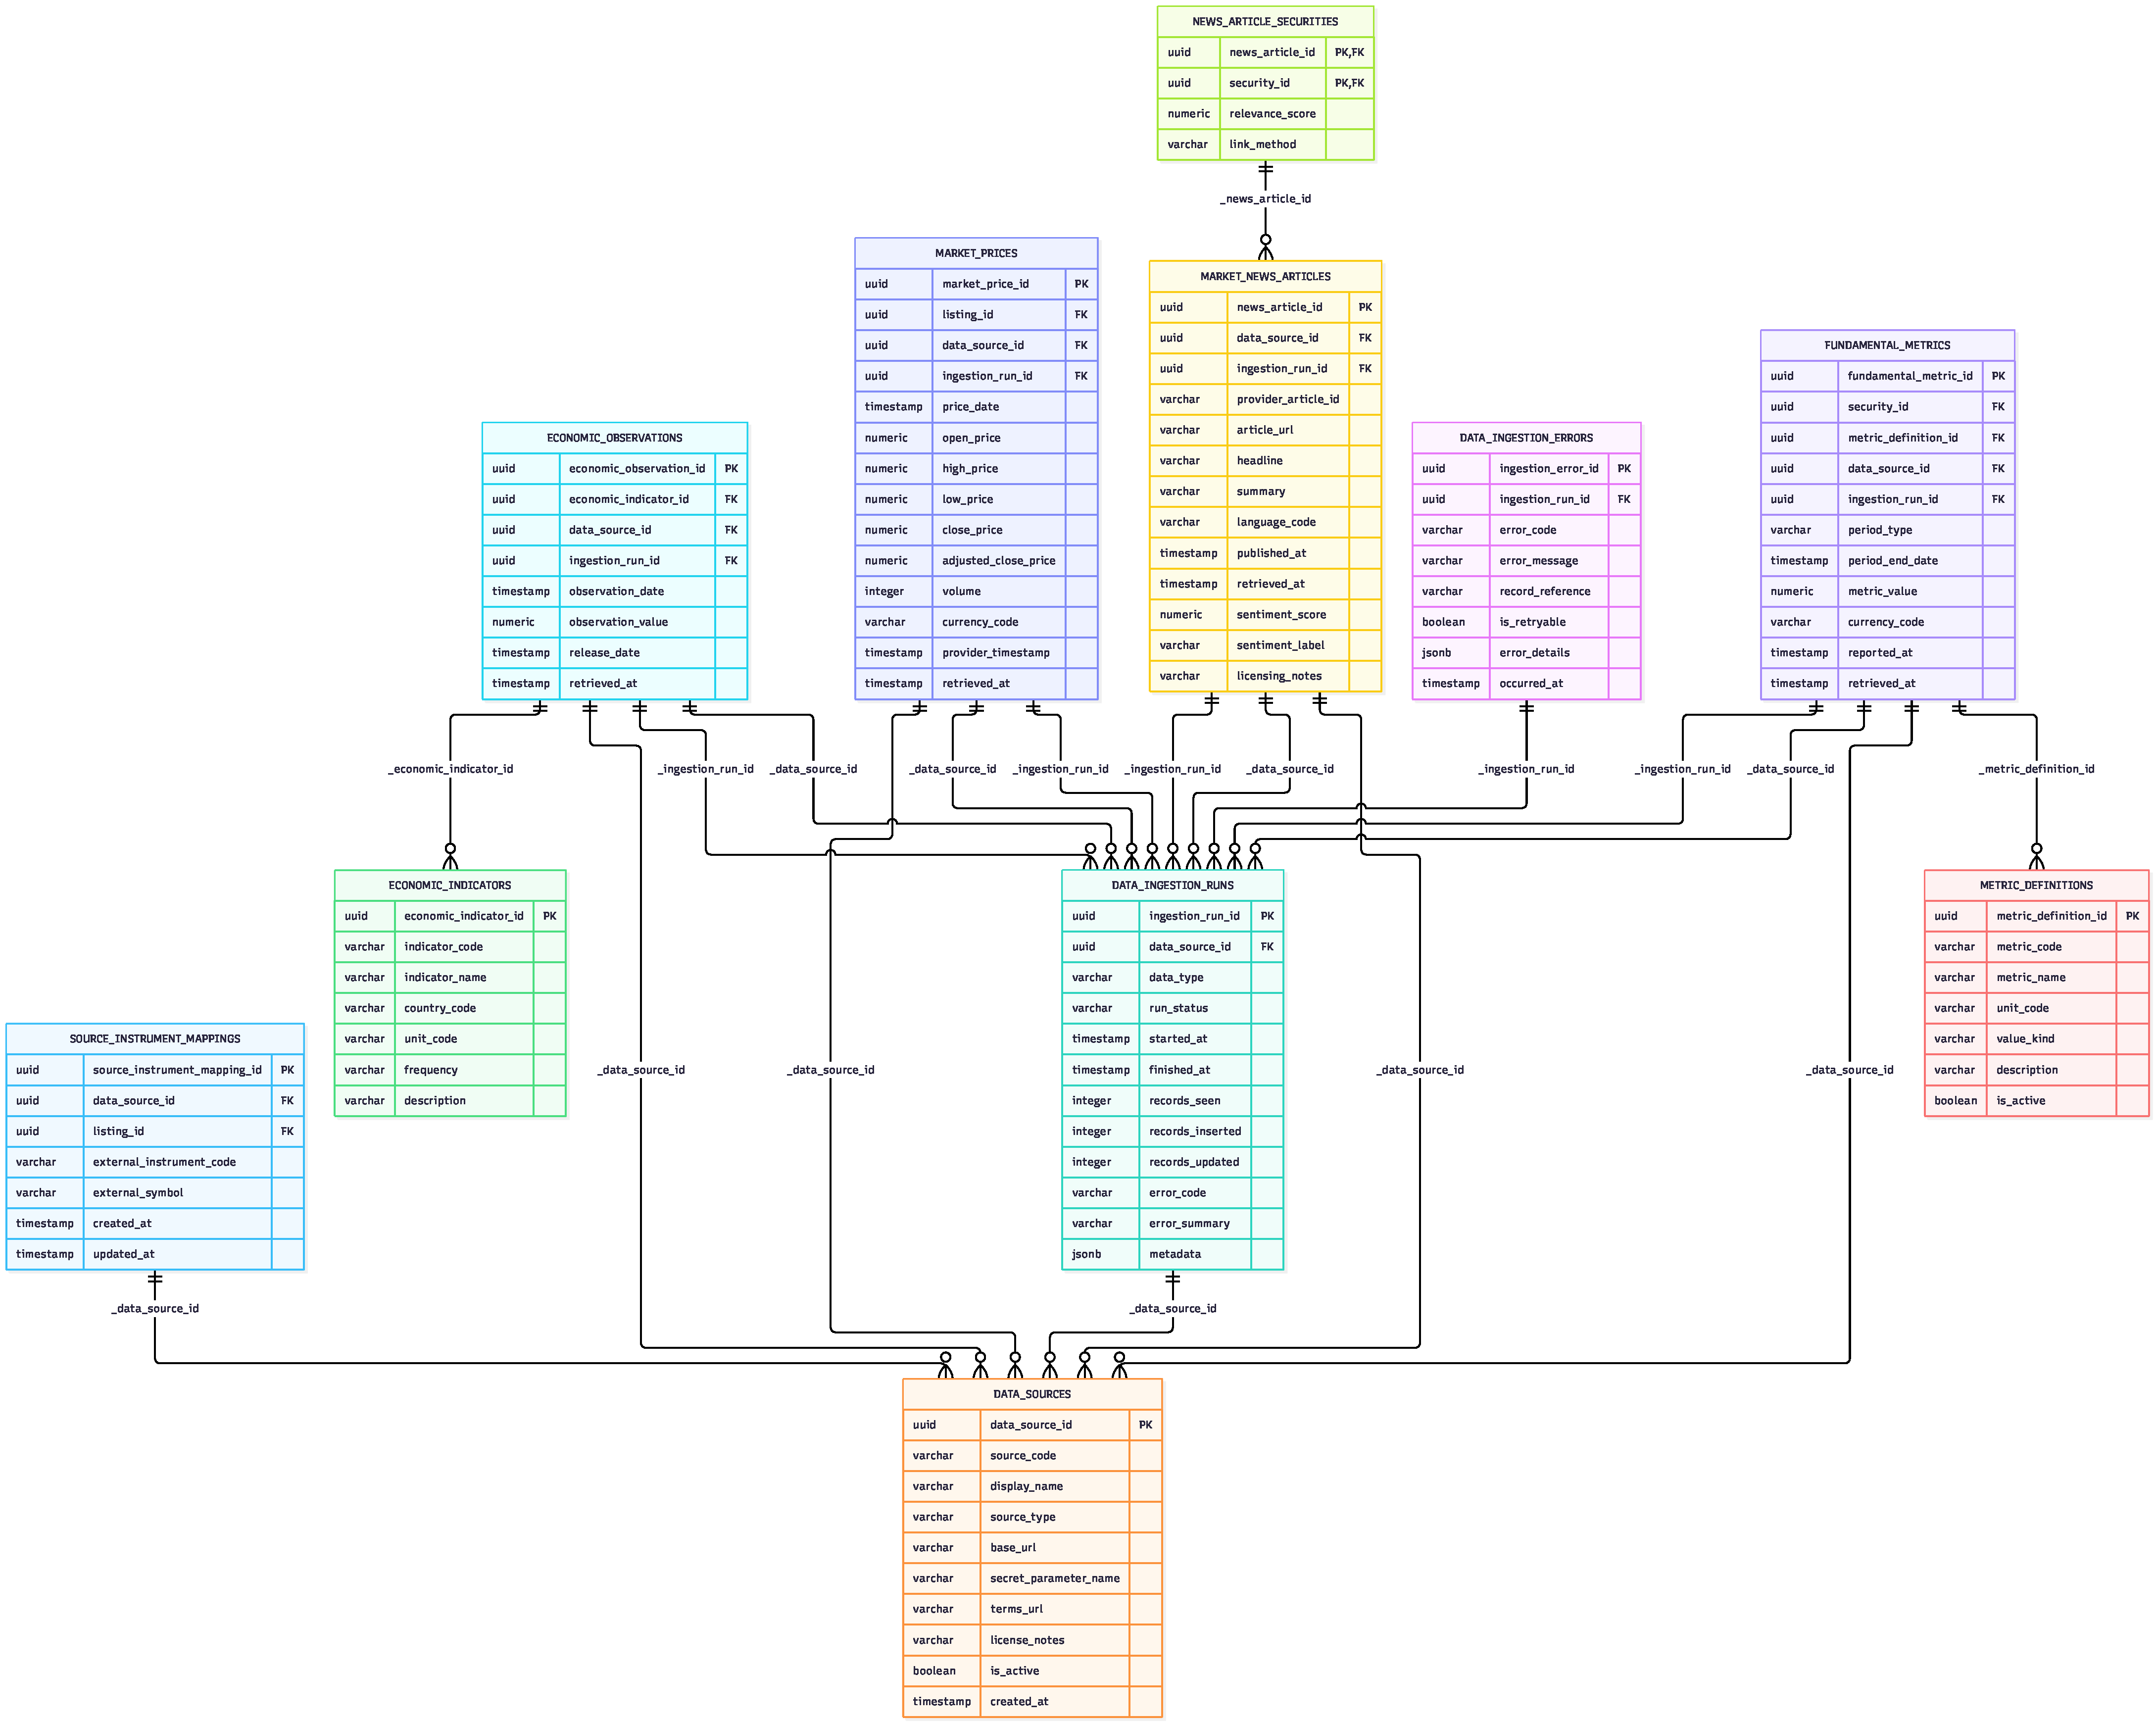
\includegraphics[width=\textwidth, height=0.72\textheight, keepaspectratio]{04_market_data_and_fundamentals_domain.pdf}
    \caption{Domain 4 ER Diagram: Market Data, Historical Quotes and Macro Regime}
    \label{fig:er_domain4}
\end{figure}

\clearpage
\subsubsection{Domain 5: Portfolio Engine, Quantitative Optimization, and Tracking}
Domain 5 forms the transactional core of Lucid, recording recommended portfolios, version histories, and daily valuations across 10 tables:
\begin{itemize}
    \item \texttt{strategy\_definitions}: Strategy templates (\textbf{Conservative}, \textbf{Moderate}, and \textbf{Aggressive}).
    \item \texttt{strategy\_versions}: Mathematical parameter sets (such as risk aversion penalties) assigned to each strategy.
    \item \texttt{investor\_portfolios}: The master account record linking each portfolio to its owner.
    \item \texttt{portfolio\_versions}: Whenever a portfolio is created or rebalanced, Lucid saves an immutable new version snapshot (Version 1, Version 2, etc.), recording the date, reason for change, and unallocated cash balance.
    \item \texttt{portfolio\_version\_constraints}: The safety limits enforced for that version (for example, no single stock exceeding 25\% and no sector exceeding 40\%).
    \item \texttt{portfolio\_generation\_requests}: An audit record of the user's input parameters (amount, goal, timeline) that triggered the portfolio creation.
    \item \texttt{portfolio\_security\_decisions}: The exact line-item stock allocations, recording the company name, recommended percentage weight, number of whole shares, purchase price, and total invested rupees.
    \item \texttt{portfolio\_performance\_snapshots}: Daily valuation records tracking the total value of the portfolio and cumulative gains or losses over time.
    \item \texttt{portfolio\_scenarios}: Projections evaluating how the portfolio would behave during major historical market crashes (such as the 2008 financial crisis or the March 2020 COVID shock).
    \item \texttt{rebalance\_suggestions}: Proposed adjustments generated by the monitoring daemon when stock prices drift away from planned targets.
\end{itemize}

Figure~\ref{fig:er_domain5} displays the Entity-Relationship structure for Domain 5:

\begin{figure}[H]
    \centering
    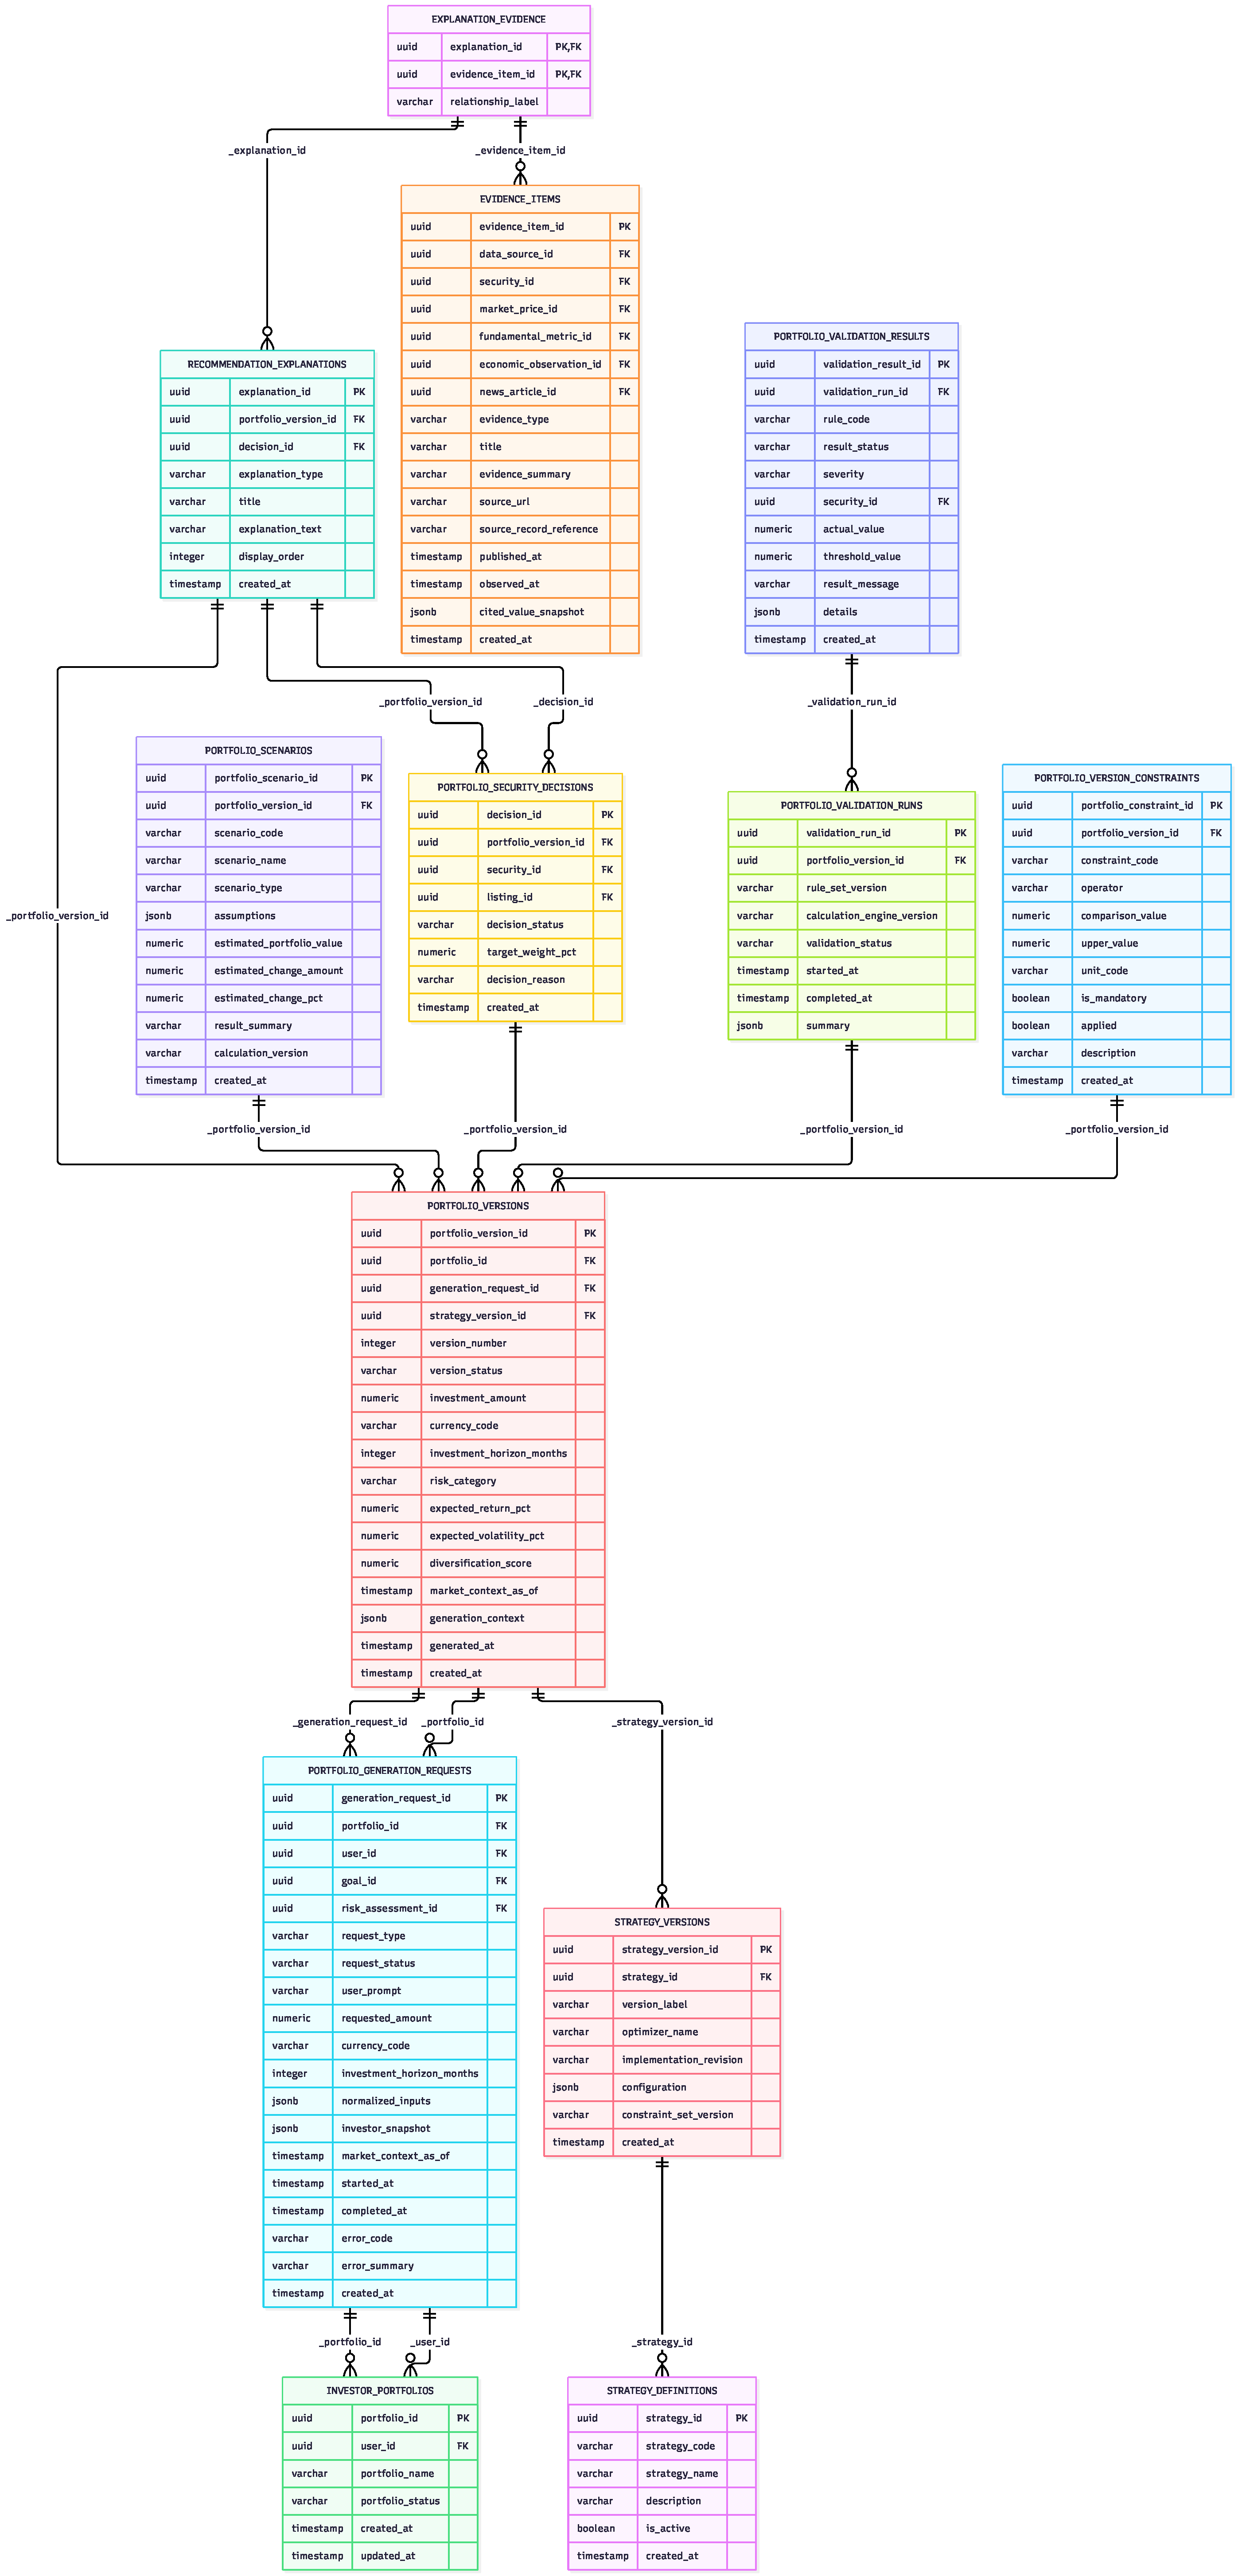
\includegraphics[width=\textwidth, height=0.72\textheight, keepaspectratio]{05_portfolio_engine_and_optimization_domain.pdf}
    \caption{Domain 5 ER Diagram: Portfolio Engine, Quantitative Optimization and Tracking}
    \label{fig:er_domain5}
\end{figure}

\clearpage
\subsubsection{Domain 6: Broker Integration, Execution, and Order Lifecycle}
Domain 6 manages connections to brokerage platforms and tracks simulated order execution across 5 tables:
\begin{itemize}
    \item \texttt{broker\_providers}: Supported brokerage platforms (such as Zerodha, Upstox, and Groww).
    \item \texttt{user\_broker\_accounts}: Securely links an investor's brokerage credentials using strong encryption.
    \item \texttt{broker\_orders}: Batches of buy and sell orders generated when an investor rebalances a portfolio.
    \item \texttt{broker\_order\_events}: Audit timeline tracking order stages (\texttt{CREATED}, \texttt{SUBMITTED}, \texttt{EXECUTED}).
    \item \texttt{broker\_executions}: The final trade execution receipts, recording filled share quantities, average purchase prices, and execution timestamps.
\end{itemize}

Figure~\ref{fig:er_domain6} displays the Entity-Relationship structure for Domain 6:

\begin{figure}[H]
    \centering
    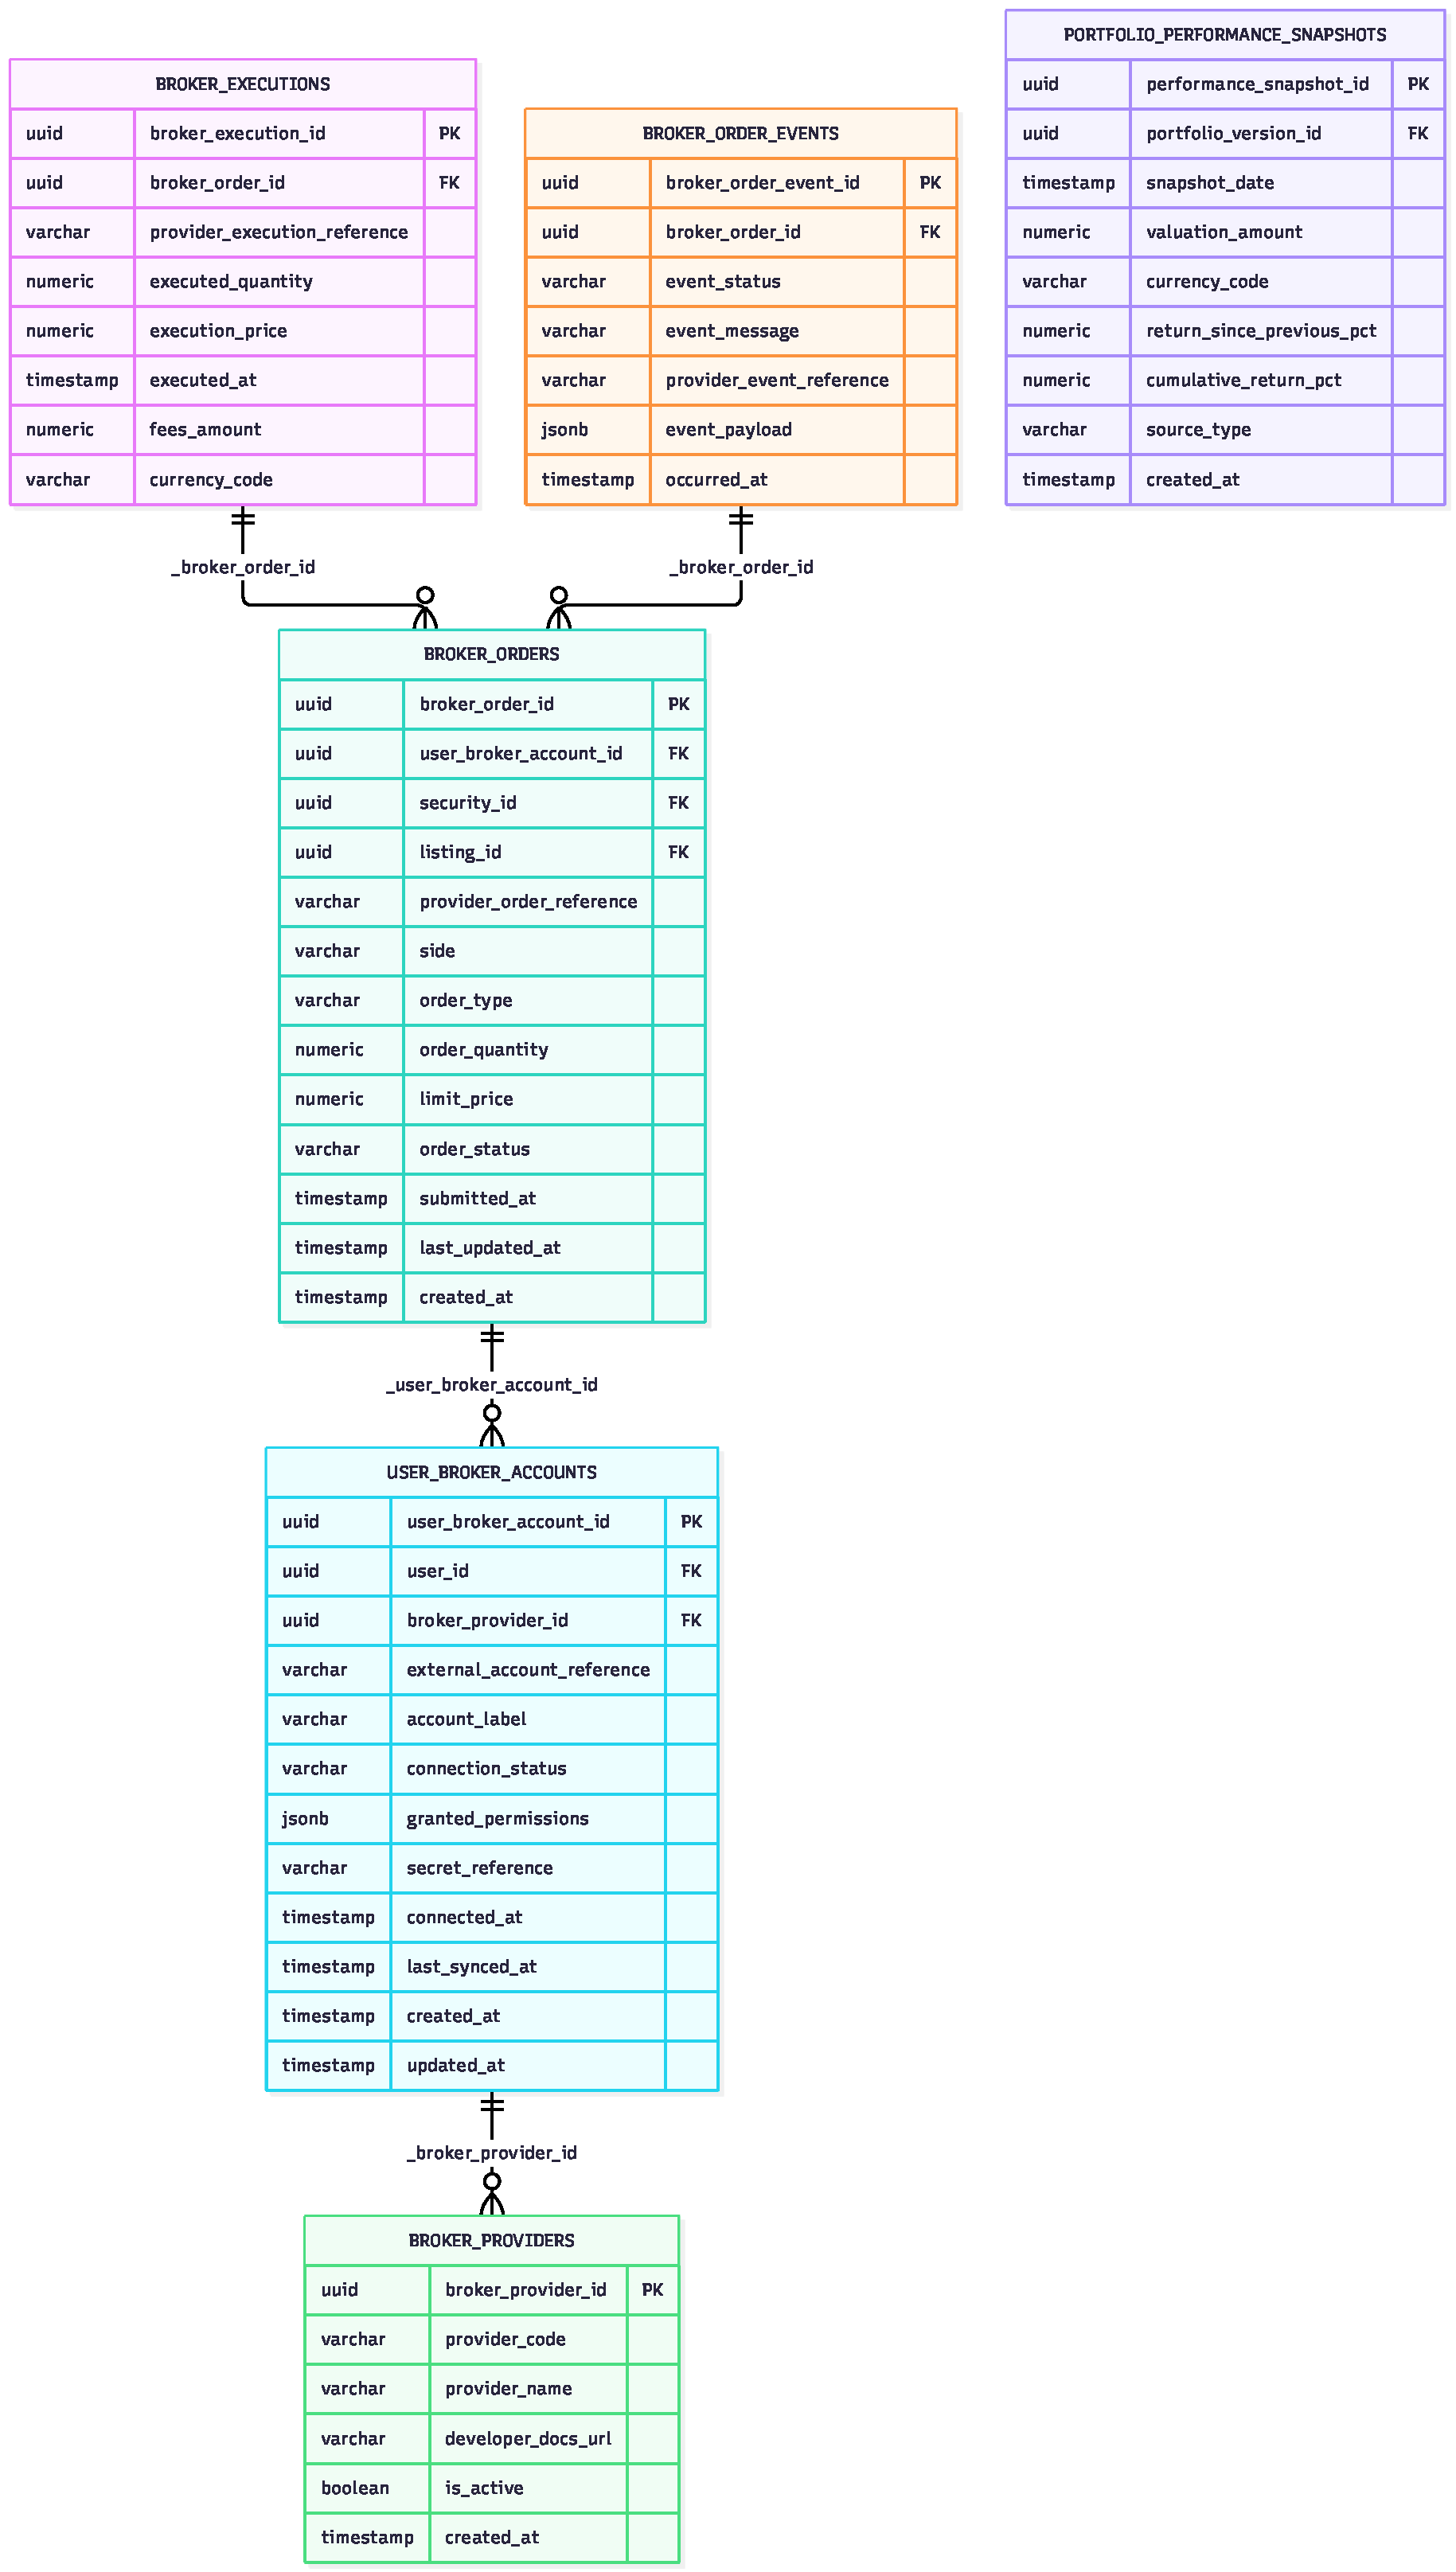
\includegraphics[width=\textwidth, height=0.72\textheight, keepaspectratio]{06_broker_integrations_and_orders_domain.pdf}
    \caption{Domain 6 ER Diagram: Broker Integration, Execution and Order Lifecycle}
    \label{fig:er_domain6}
\end{figure}

\clearpage
\subsubsection{Domain 7: Demat CAS Diagnosis and Portfolio Analytics}
Domain 7 stores imported external Demat portfolios and health diagnostic assessments across 3 tables:
\begin{itemize}
    \item \texttt{existing\_portfolios}: Records of uploaded monthly Demat statements (via PDF CAS statement or manual entry).
    \item \texttt{existing\_portfolio\_holdings}: The parsed holdings extracted from the statement (company ISIN, share quantities, and original purchase costs).
    \item \texttt{portfolio\_diagnoses}: The complete diagnostic report, including total current valuation, sector concentration risk, the Herfindahl-Hirschman Index (HHI) diversification score, and actionable hold, buy, or trim recommendations.
\end{itemize}

Figure~\ref{fig:er_domain7} displays the Entity-Relationship structure for Domain 7:

\begin{figure}[H]
    \centering
    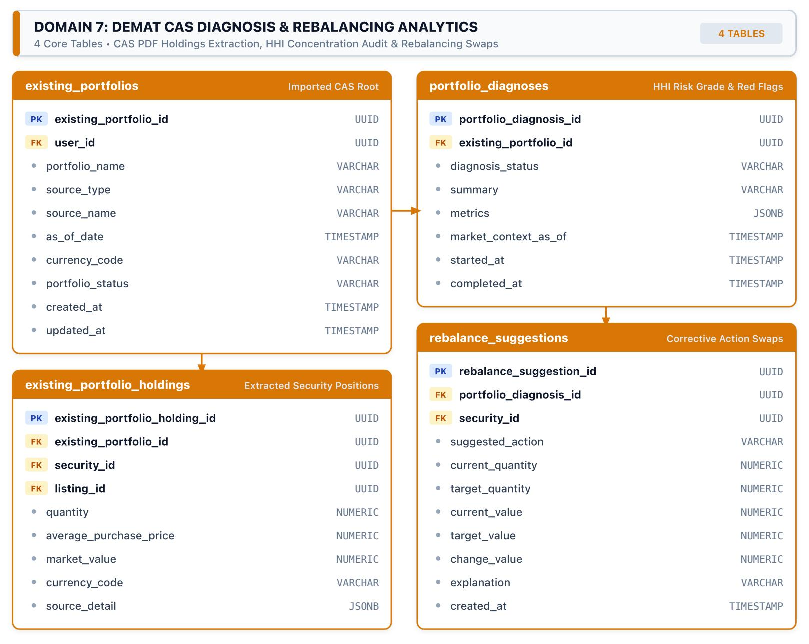
\includegraphics[width=\textwidth, height=0.72\textheight, keepaspectratio]{07_demat_diagnosis_and_rebalancing_domain.pdf}
    \caption{Domain 7 ER Diagram: Demat CAS Diagnosis and Portfolio Analytics}
    \label{fig:er_domain7}
\end{figure}

\clearpage
\subsubsection{Domain 8: Multi-Agent AI Telemetry, Reasoning Traces, and Audits}
Domain 8 stores the execution logs of the AI agents, plain-English explanations, and real-time user alerts across 13 tables:
\begin{itemize}
    \item \texttt{agent\_definitions}: Master catalog of the 13 specialized AI roles (Macro, Fundamental, News, Critic, etc.).
    \item \texttt{agent\_versions}: Tracks versions of agent prompts and model settings over time.
    \item \texttt{agent\_execution\_runs}: Audit log recording how long each agent took to think, token costs, and structured outputs.
    \item \texttt{recommendation\_explanations}: The plain-English ``Stock-Why'' justifications and financial metric breakdowns shown to the user.
    \item \texttt{evidence\_items}: Verifiable factual data points (such as company profit numbers or RBI interest rate quotes) that support the explanations.
    \item \texttt{explanation\_evidence}: Connects each explanation to its specific supporting evidence items.
    \item \texttt{portfolio\_validation\_runs}: Audit logs verifying that portfolios satisfy mathematical rules.
    \item \texttt{portfolio\_validation\_results}: Pass/fail audit records for rules.
    \item \texttt{data\_sources}: Directory of external data providers (NSE, BSE, Yahoo Finance).
    \item \texttt{data\_ingestion\_runs}: Execution logs of automated nightly price and news download jobs.
    \item \texttt{data\_ingestion\_errors}: Detailed error logs capturing any API failures or bad data records.
    \item \texttt{notifications}: Real-time investor alerts (such as portfolio drift notices and rebalancing recommendations).
    \item \texttt{user\_feedback}: User ratings and comments on whether an explanation was clear and helpful.
\end{itemize}

Figure~\ref{fig:er_domain8} displays the Entity-Relationship structure for Domain 8:

\begin{figure}[H]
    \centering
    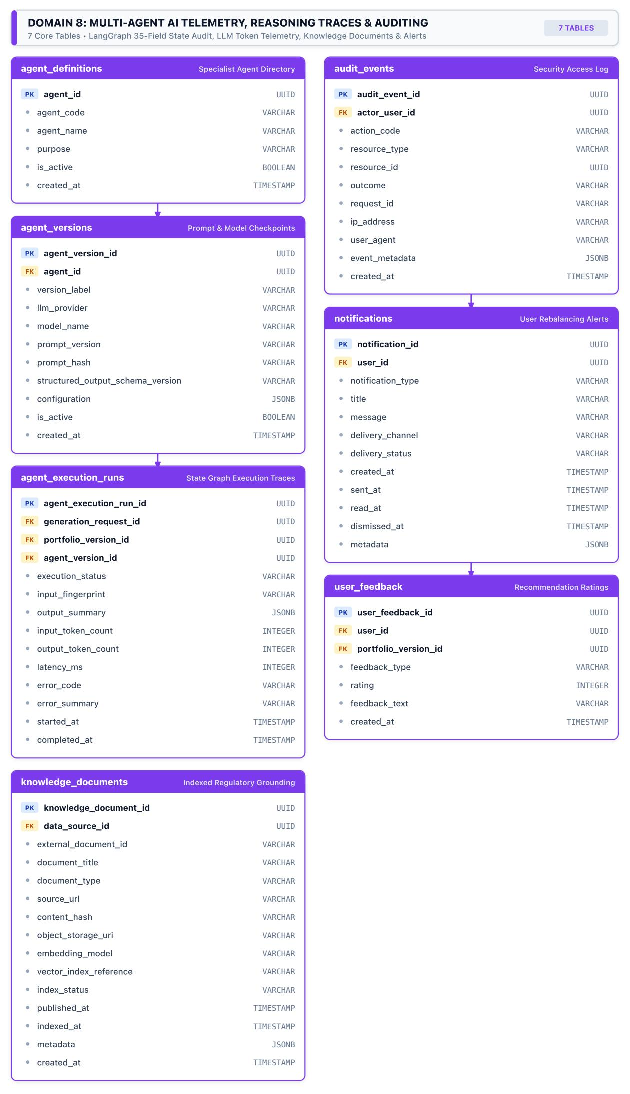
\includegraphics[width=\textwidth, height=0.72\textheight, keepaspectratio]{08_multi_agent_telemetry_and_auditing_domain.pdf}
    \caption[Domain 8 ER Diagram: AI Telemetry and Verification]{Domain 8 ER Diagram: Multi-Agent AI Telemetry, Reasoning Traces and Verification}
    \label{fig:er_domain8}
\end{figure}

\subsection{Database Design: Speed and Safety}
To ensure the database runs quickly and reliably, four key engineering choices were made:
\begin{enumerate}
    \item \textbf{High Speed with Structured Flexibility}: Core tables (users, portfolios, stock prices) follow strict relational rules to prevent duplicate or conflicting records. At the same time, complex analysis reports (such as sector concentration breakdowns and AI factor scores) are stored in structured JSON columns (\texttt{JSONB}). This allows the web dashboard to load complete portfolio screens in less than 5 milliseconds without running dozens of separate database queries.
    \item \textbf{Secure Universal IDs (UUIDs)}: Every account, portfolio, and order uses a randomized 128-bit universal identifier (UUID) instead of a simple number like 1, 2, or 3. This protects user privacy by preventing unauthorized parties from guessing other users' portfolio links.
    \item \textbf{Fast Search Indexes}: Searching through thousands of daily stock prices or looking up companies by ticker symbol is made nearly instantaneous by creating specialized B-Tree search indexes on frequently queried columns (such as \texttt{securities.isin} and \texttt{market\_prices.price\_date}).
    \item \textbf{Accidental Deletion Protection}: Strong database rules (called \textbf{foreign key constraints}) protect financial records. For example, deleting a user account is strictly blocked if active transaction ledgers or historical investment records exist, ensuring that audit trails can never be accidentally erased.
\end{enumerate}

\section{Datasets Used and External Data Sources}
\label{sec:dataset}

\subsection{Overview of Data Sources: What Information Lucid Uses}
To make intelligent investment recommendations, a financial system needs reliable, up-to-date information about companies, market prices, and the broader economy. Just as a human investor reads newspapers, reviews company annual reports, and checks stock exchange prices, Lucid collects data from verified official sources.

Lucid relies on five primary categories of data:
\begin{enumerate}
    \item \textbf{Stock Exchange Directories (NSE and BSE)}: The official registers of actively traded companies in India, including company names, exchange ticker symbols, and unique international identification numbers (called \textbf{ISINs}).
    \item \textbf{Historical Market Prices}: Daily trading prices (Open, High, Low, Close, and Volume) over the past 252 trading sessions (one full year) for every listed company.
    \item \textbf{Corporate Financial Fundamentals}: Vital balance sheet health metrics retrieved from quarterly financial reports, such as Return on Equity (ROE), Debt-to-Equity ratios, and Price-to-Earnings (P/E) ratios.
    \item \textbf{Macroeconomic Benchmarks from the Reserve Bank of India (RBI)}: Crucial national economic numbers, including the official RBI policy repo rate (6.50\%), inflation rates, and 10-year Indian government bond yields.
    \item \textbf{Financial News and Corporate Announcements}: Curated headlines and articles from recognized Indian business publications to identify company developments, legal risks, or management changes.
\end{enumerate}

Figure~\ref{fig:api_to_agent} illustrates how raw external information is downloaded, cleaned, stored in PostgreSQL, and converted into structured summaries for the AI agents:

\clearpage
\begin{figure}[p]
    \centering
    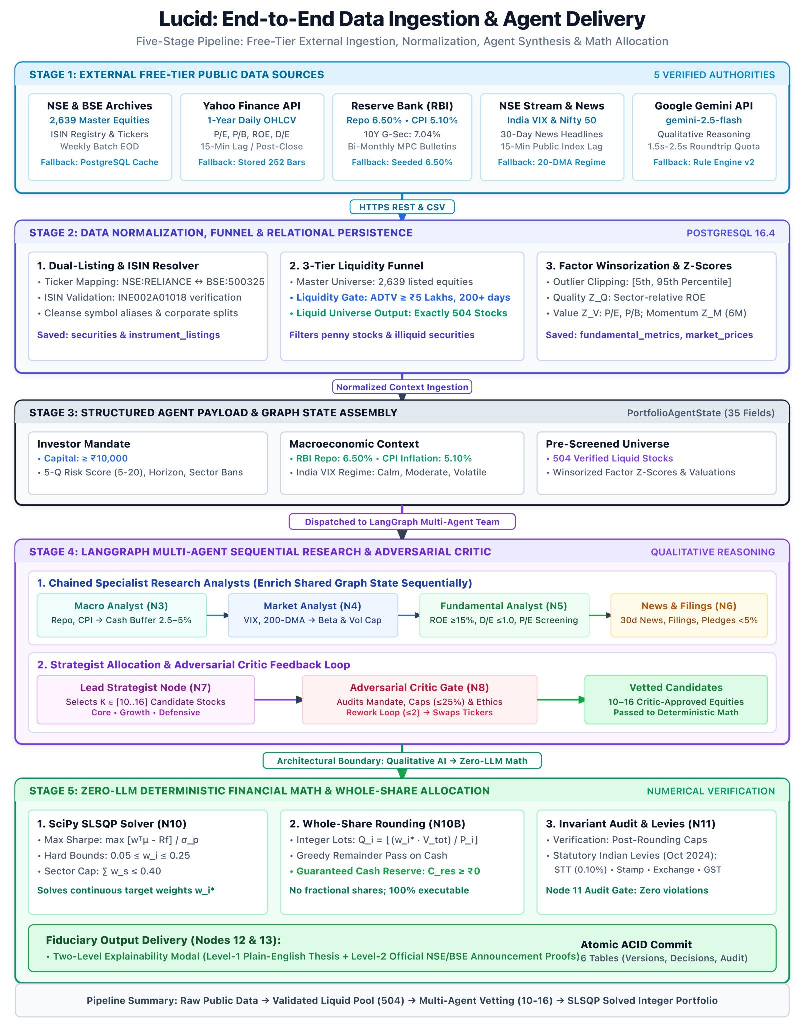
\includegraphics[width=\textwidth, keepaspectratio]{API_TO_AGENT_DATA_FLOW.pdf}
    \caption{Data Ingestion, Transformation, and Agent Payload Delivery Pipeline}
    \label{fig:api_to_agent}
\end{figure}
\clearpage

\subsection{Inventory of External Data Sources}
Table~\ref{tab:external_data_sources} provides a comprehensive overview of every external data source integrated into Lucid, explaining what information is retrieved, its update frequency and associated delay profile, its primary purpose, and what fallback safety measure is used if a provider is temporarily unavailable:

\begin{table}[H]
\centering
\small
\caption{Lucid External Data-Source Inventory and Ingestion Parameters}
\label{tab:external_data_sources}
\resizebox{\textwidth}{!}{%
\begin{tabular}{lllll}
\toprule
\textbf{Data Source / Authority} & \textbf{Data Retrieved} & \textbf{Update Frequency \& Delay Profile} & \textbf{Primary Purpose} & \textbf{Offline Fallback Safety} \\
\midrule
\textbf{National Stock Exchange (NSE)} & Active stock list, ISINs, tickers & Weekly EOD / 15-Min Delayed Index & Security master catalog & Cached PostgreSQL records \\
\textbf{Bombay Stock Exchange (BSE)} & Dual-listed tickers \& scrip codes & Monthly batch sync & Cross-exchange ticker mapping & Primary NSE ticker records \\
\textbf{Yahoo Finance (\texttt{yfinance})} & 1-Year daily price bars (OHLCV) & Daily after 16:30 IST (15-Min Intraday Lag) & Volatility and covariance matrix & Stored historical price database \\
\textbf{Yahoo Finance Fundamentals} & P/E, P/B, ROE, Debt/Equity, MCAP & Weekly batch / Quarterly filing lag & Balance sheet health screening & Cached \texttt{fundamental\_metrics} \\
\textbf{Reserve Bank of India (RBI)} & Repo Rate (6.50\%), CPI (5.10\%) & Bi-monthly MPC / 2--3 week inflation lag & Macroeconomic regime score & Seeded 6.50\% baseline \\
\textbf{NSE Index Stream} & India VIX \& Nifty 50 Index & 15-Minute statutory delayed public feed & Market volatility tiering & 20-Day moving average \\
\textbf{Google Gemini API} & Qualitative analysis \& agent reasoning & 1.5s--2.5s network roundtrip (Free quota) & Contextual reasoning & 0.48s Rule Engine (\texttt{fiduciary-rule-engine-v2}) \\
\bottomrule
\end{tabular}%
}
\end{table}

\subsubsection{Free-Tier API Data Delays and Real-Time Limitations}
Because Lucid connects to public free-tier endpoints rather than dedicated institutional feeds, each external data provider introduces specific operational delays:
\begin{enumerate}
    \item \textbf{15-Minute Statutory Exchange Delay (Yahoo Finance and NSE Public Streams)}: 
    Public market data feeds provided by Yahoo Finance (\texttt{yfinance}) and the National Stock Exchange public web portal are legally restricted by Indian exchange regulations to a \textbf{15-minute statutory delay} during live market hours (09:15 to 15:30 IST). Free endpoints do not supply sub-second, tick-by-tick Level 2 (order depth) or Level 3 (order queue) feeds. As a result, intraday quotes, stock prices, and the India VIX index reflect market conditions from 15 minutes prior.
    
    \item \textbf{End-of-Day (EOD) Settlement and Historical Data Finalization}: 
    Historical daily price candles (Open, High, Low, Close, and Volume) are published in batch after exchange trading closes. Yahoo Finance finalizes official closing prices and corporate action adjustments only after \textbf{16:30 IST}. Intraday historical bars on free endpoints can occasionally experience missing candles or rate-limiting during peak market volatility hours.
    
    \item \textbf{Quarterly and Bi-Monthly Macroeconomic Reporting Lags}: 
    Fundamental corporate financial statements (quarterly earnings, debt levels, and Return on Equity) are updated on a quarterly reporting cycle following company disclosures to stock exchanges. Similarly, official macroeconomic data from the Reserve Bank of India (RBI) is updated \textbf{bi-monthly} following scheduled Monetary Policy Committee (MPC) meetings, while Ministry of Statistics and Programme Implementation (MoSPI) inflation statistics (CPI) are released monthly with an inherent two-to-three-week reporting lag. Free public endpoints cannot provide continuous real-time macroeconomic updates because the underlying governmental sources publish periodically.
    
    \item \textbf{Cloud AI Network Latency and Free Quota Throttling}: 
    The Google Gemini 3.8 Flash language model communicates with the backend via HTTPS cloud requests. Under free-tier and standard API developer tiers, each prompt incurs a \textbf{1.5-second to 2.5-second network roundtrip latency}. Additionally, free developer tiers enforce rate limits (such as 15 requests per minute). If multiple users generate portfolios simultaneously, free endpoints risk experiencing temporary HTTP 429 (Too Many Requests) throttling.
\end{enumerate}

\paragraph{Why API Delays Do Not Impact Lucid's Investment Premise}
While a 15-minute price delay would be catastrophic for high-frequency day-trading algorithms that attempt to profit from millisecond price fluctuations, it has virtually \textbf{zero adverse impact} on Lucid's investment performance. 

Lucid is designed specifically for \textbf{goal-driven, medium-to-long-term investing} with investment horizons extending from 3 months to 30 years (360 months):
\begin{itemize}
    \item \textbf{Mathematical Invariance of Risk Models}: Quantitative portfolio optimization relies on expected returns ($\boldsymbol{\mu}$) and the asset covariance matrix ($\Sigma_{\text{reg}}$) computed across 252 full trading sessions (one full year of daily closing prices). A 15-minute intraday fluctuation changes a stock's 252-day annual volatility by less than $0.01\%$. Mathematically, the resulting Markowitz optimal weights and integer share quantities are identical whether calculated on a 15-minute delayed price or a tick-level price.
    \item \textbf{Macro and Fundamental Stability}: Company balance sheet ratios (such as ROE $\ge 15\%$ or Debt/Equity $\le 1.0$) represent long-term operational health that remains stable across months. A 15-minute price lag does not change the financial health of HDFC Bank or Tata Consultancy Services.
    \item \textbf{Disciplined 5\% Drift Bands}: Lucid's background monitoring evaluates portfolio drift against a 5\% tolerance band. In real-world Indian equity markets, a diversified blue-chip portfolio typically takes several days or weeks of continuous price drift to breach a 5\% rebalancing trigger, making intraday millisecond price precision unnecessary.
\end{itemize}

\paragraph{Architectural Safeguards Against Free-Tier API Delays and Failures}
To ensure complete transparency and system reliability despite free-tier API constraints, Lucid implements three architectural safeguards:
\begin{enumerate}
    \item \textbf{User Interface Freshness Badges}: Every stock quote, portfolio valuation, and performance chart in the frontend displays an explicit data freshness chip (such as \texttt{15-MIN DELAYED}, \texttt{END OF DAY}, or \texttt{CACHED BASELINE}). The retail investor is always fully aware of the data timestamp and is never misled into believing delayed information is real-time streaming.
    \item \textbf{PostgreSQL Resilient Caching}: All retrieved price records, exchange directories, and fundamental metrics are stored locally in the PostgreSQL database. If an external free API is throttled, experiences downtime, or fails to respond, Lucid automatically serves the most recent cached records, allowing the user to generate or inspect portfolios without failure.
    \item \textbf{Deterministic 0.48-Second Fallback Circuit-Breaker}: If the Google Gemini cloud API encounters network latency or hits free-tier rate limits, the LangGraph workflow instantly switches to the deterministic local rule engine (\texttt{fiduciary-rule-engine-v2}). This local engine selects pre-vetted liquid stocks and calculates optimal allocations in just \textbf{0.48 seconds}, ensuring the application never freezes or times out.
\end{enumerate}

\subsection{Exchange Universe Coverage and Synchronization}

\subsubsection{Why Unique Company Identification (ISIN) Matters}
In India, a single company can have different names and ticker symbols across different platforms. For example, Tata Consultancy Services is traded as \texttt{TCS} on the National Stock Exchange (NSE) and as scrip code \texttt{532540} on the Bombay Stock Exchange (BSE). Furthermore, companies occasionally split their shares or change their corporate names.

To prevent confusion and eliminate duplicate entries, Lucid uses the \textbf{International Securities Identification Number (ISIN)}. An ISIN is a globally standardized 12-character alphanumeric code (such as \texttt{INE467B01029} for TCS) that permanently and uniquely identifies a security, regardless of which exchange it is traded on or what nickname it has.

\subsubsection{Resolving Corporate Splits and Duplicate Codes}
When corporate actions occur, companies may update their ISINs. Lucid's synchronization service (\texttt{exchange\_universe\_sync.py}) includes automated conflict resolution logic (\texttt{ON CONFLICT (isin) DO UPDATE}):
\begin{itemize}
    \item When \textbf{Bajaj Finance Ltd.} underwent a stock split from a face value of Rs.~10 to Rs.~2, its ISIN changed from \texttt{INE296A01016} to \texttt{INE296A01024}. Lucid recognized the corporate event, updated the active security identifier, and preserved all previous historical price records seamlessly.
    \item Similar split events for \textbf{Dr.~Reddy's Laboratories} and \textbf{Hindustan Aeronautics Ltd. (HAL)} were handled automatically without creating orphan records or crashing the database.
\end{itemize}

\subsubsection{Scale of the Active Investment Universe}
As verified in PostgreSQL:
\begin{itemize}
    \item \textbf{Total Cataloged Listed Equities}: Exactly \textbf{2,639 listed Indian companies} stored in the \texttt{securities} table.
    \item \textbf{Total Exchange Trading Listings}: Exactly \textbf{2,715 trading listings} in the \texttt{instrument\_listings} table (including dual listings across the NSE and BSE).
    \item \textbf{Active Recommendation Eligibility}: All 2,639 listed equities are dynamically screened based on investor risk capacity, institutional liquidity thresholds, and price data freshness.
    \item \textbf{Complete Coverage for Search and Statement Diagnostics}: All 2,639 stocks are instantly searchable in the user interface and fully recognized when users upload monthly Demat CAS statements.
\end{itemize}

\subsection{Historical Price Data and Statistical Calculations}
To calculate investment risks and expected returns, Lucid analyzes 252 consecutive trading sessions (one standard financial year) stored in the \texttt{market\_prices} table:

\begin{enumerate}
    \item \textbf{Daily Logarithmic Returns}:
    Instead of simple percentage changes, quantitative finance uses logarithmic returns because they are additive across time:
    \begin{equation}
    r_{i,t} = \ln \left( \frac{P_{i,t}^{\text{adjusted}}}{P_{i,t-1}^{\text{adjusted}}} \right)
    \end{equation}
    where $P_{i,t}^{\text{adjusted}}$ is the closing stock price adjusted for any dividends or stock splits.
    \item \textbf{Covariance Matrix ($\mathbf{\Sigma}$)}:
    To measure how different stocks move in relation to one another, Lucid calculates the sample covariance matrix across all shortlisted candidates:
    \begin{equation}
    \Sigma_{ij} = \frac{1}{T-1} \sum_{t=1}^{T} (r_{i,t} - \bar{r}_i)(r_{j,t} - \bar{r}_j)
    \end{equation}
    To convert daily covariance into annual terms, the matrix is multiplied by the annual trading day factor ($\sqrt{252}$).
\end{enumerate}

\subsection{Data Delivery: Feeding Clean Information to AI Agents}
A foundational architectural rule in Lucid is that \textbf{raw, unstructured API data is never dumped directly into the AI language model}.

Dumping raw website data or huge JSON files into an AI prompt causes three serious problems:
\begin{enumerate}
    \item It wastes expensive AI context tokens.
    \item It significantly slows down response times for the end user.
    \item It overwhelms the AI model with irrelevant information, increasing the risk of hallucinated or inaccurate conclusions.
\end{enumerate}

Instead, Lucid acts as a strict filter. Backend Python services process, clean, and verify external market data first, packaging only the essential, relevant fields into compact JSON payloads for each specialist agent.

Table~\ref{tab:agent_payloads} lists the exact structured data delivered to each agent:

\begin{table}[H]
\centering
\caption{Exact Data Payloads Delivered to LangGraph Multi-Agent Nodes}
\label{tab:agent_payloads}
\resizebox{\textwidth}{!}{%
\begin{tabular}{lllp{6cm}}
\toprule
\textbf{Agent Node} & \textbf{Data Source} & \textbf{Raw Data Format} & \textbf{Exact Structured Fields Delivered to Agent} \\
\midrule
\textbf{Input Validator} & User Web Form & JSON Payload & \texttt{capital\_inr}, \texttt{risk\_category}, \texttt{time\_horizon\_years}, \texttt{goal\_name}, \texttt{excluded\_sectors} \\
\textbf{Macro Analyst} & RBI Policy Bulletins & HTML / Reports & \texttt{rbi\_repo\_rate\_pct}, \texttt{inflation\_cpi\_pct}, \texttt{gdp\_forecast}, \texttt{monetary\_stance} \\
\textbf{Market Regime} & NSE Index Streams & Live Quotes & \texttt{india\_vix\_value}, \texttt{vix\_tier}, \texttt{nifty\_current}, \texttt{nifty\_50\_dma}, \texttt{regime\_trend} \\
\textbf{Universe Selector} & PostgreSQL Master & SQL Records & Filtered candidates: \texttt{symbol}, \texttt{company\_name}, \texttt{sector}, \texttt{liquidity\_tier} \\
\textbf{Fundamental Analyst} & Yahoo Finance / DB & Balance Sheets & Per Candidate: \texttt{symbol}, \texttt{pe\_ratio}, \texttt{pb\_ratio}, \texttt{roe\_pct}, \texttt{debt\_to\_equity} \\
\textbf{News Analyst} & Curated Ingested News & Text Articles & Per Candidate: \texttt{symbol}, \texttt{headline\_count}, \texttt{sentiment\_score}, \texttt{legal\_risk\_flags} \\
\textbf{Adversarial Critic} & Preceding Agent State & Python Dictionary & Candidate shortlist, proposed sector weights, identified risk factors \\
\textbf{SLSQP Optimizer} & Quant Service & Math Arrays & Covariance matrix $\mathbf{\Sigma}$, expected returns $\boldsymbol{\mu}$, risk-free rate $R_f$, budget bounds \\
\textbf{Explainability Node} & Portfolio Decisions & DB Records & Final chosen symbols, allocated shares, weights, Sharpe score, risk contributions \\
\bottomrule
\end{tabular}%
}
\end{table}

\subsubsection{Example of a Sanitized Agent Payload}
Below is a real example of the clean, focused data package sent to the \textbf{Fundamental Analyst Agent}:

\begin{footnotesize}
\begin{verbatim}
{
  "macro_context": {
    "repo_rate": 6.50,
    "vix_tier": "Normal Volatility (14.2)",
    "market_trend": "Bullish above 200-DMA"
  },
  "candidate_stocks": [
    {
      "symbol": "TCS",
      "company": "Tata Consultancy Services Ltd.",
      "sector": "Information Technology",
      "pe_ratio": 28.4,
      "roe_pct": 46.2,
      "debt_to_equity": 0.08
    },
    {
      "symbol": "HDFCBANK",
      "company": "HDFC Bank Ltd.",
      "sector": "Financial Services",
      "pe_ratio": 18.9,
      "roe_pct": 16.8,
      "debt_to_equity": 1.12
    }
  ]
}
\end{verbatim}
\end{footnotesize}

By providing only verified, essential numbers, the AI agent can complete its evaluation quickly, reliably, and without confusion.

\section{API Contract and Integration Design}
\label{sec:api_contract}

\subsection{What is an API and Why Does Lucid Use One?}
To understand how Lucid's website communicates with its calculation engine, it helps to use the analogy of a restaurant:
\begin{itemize}
    \item \textbf{The Customer (The User Interface / Frontend)}: The investor interacts with buttons, forms, and charts displayed in their web browser (built with Next.js and React).
    \item \textbf{The Kitchen (The Backend Server and Database)}: The backend server runs the 13 AI agents, accesses 2,639 listed Indian companies, and executes mathematical solvers to optimize portfolios.
    \item \textbf{The Waiter (The API)}: An \textbf{Application Programming Interface (API)} acts as the professional waiter. When the investor clicks ``Generate Portfolio,'' the waiter takes the customer's order to the kitchen, ensures the kitchen prepares it according to the customer's rules, and brings the final dish (the recommended portfolio) back to the table in a clean, organized format.
\end{itemize}

Because Lucid's frontend and backend are decoupled, the website never touches the database directly. Every interaction occurs through secure, standardized API messages.

\subsection{Core Rules of Lucid's API Communication}
Lucid follows four foundational design principles to ensure fast, secure, and reliable communication:
\begin{enumerate}
    \item \textbf{Standardized Base URL and Versioning}: All API routes begin with the prefix \texttt{/api/v1/}. Versioning ensures that if new features are added in the future (such as \texttt{/api/v2/}), existing apps continue working without breaking.
    \item \textbf{Secure Digital Session Badges (JWT Tokens)}: When a user logs in, the server gives them a temporary, cryptographically signed digital pass (called a \textbf{JSON Web Token} or JWT). For every subsequent action (such as saving a goal or checking holdings), the browser presents this badge in the request header (\texttt{Authorization: Bearer <token>}). This proves the user's identity without requiring them to re-enter their password for every click. Tokens expire after 60 minutes for safety.
    \item \textbf{Strict Input Inspection (Pydantic v2)}: The server inspects every incoming message before processing it. If a user tries to enter negative money, an invalid email address, or an unrecognized stock ticker, the server immediately stops the request and returns a friendly error message, protecting the system from bad data.
    \item \textbf{Predictable Status Codes}: Lucid uses standard international web response codes:
    \begin{itemize}
        \item \texttt{200 OK}: The request was successful, and the requested information is returned.
        \item \texttt{201 Created}: A new record (such as a newly generated portfolio or saved financial goal) was created successfully.
        \item \texttt{400 Bad Request}: The request contained invalid information (such as entering an investment amount below the minimum Rs.~5,000 threshold).
        \item \texttt{401 Unauthorized}: The user has not logged in or their session token has expired.
        \item \texttt{429 Too Many Requests}: The user is sending requests too quickly, activating rate-limiting protections.
        \item \texttt{500 Internal Server Error}: An unexpected technical error occurred on the server.
    \end{itemize}
\end{enumerate}

\subsection{Complete API Inventory: 82 Active Endpoints}
The Lucid backend provides exactly \textbf{82 unique API endpoints} organized into eleven functional groups, as detailed in Table~\ref{tab:api_domain_inventory}:

\begin{table}[H]
\centering
\caption{Lucid Complete API Endpoint Domain Inventory (82 Endpoints)}
\label{tab:api_domain_inventory}
\resizebox{\textwidth}{!}{%
\begin{tabular}{lcl}
\toprule
\textbf{Functional API Domain} & \textbf{Routes} & \textbf{Primary Routes and Key Operations} \\
\midrule
\textbf{1. Authentication \& Security} & 8 & \texttt{/auth/login}, \texttt{/auth/register}, \texttt{/auth/logout}, \texttt{/auth/me}, \texttt{/auth/change-password} \\
\textbf{2. User Profile \& Preferences} & 6 & \texttt{/profile}, \texttt{/profile/preferences}, \texttt{/profile/security-preferences}, \texttt{/profile/sector-preferences} \\
\textbf{3. Financial Goal Management} & 5 & \texttt{/goals}, \texttt{/goals/\{id\}}, \texttt{/goals/\{id\}/progress}, \texttt{/goals/\{id\}/link-portfolio} \\
\textbf{4. Risk Questionnaire \& Scoring} & 5 & \texttt{/risk-questions}, \texttt{/risk-questions/\{id\}}, \texttt{/risk-assessments}, \texttt{/risk-assessments/latest} \\
\textbf{5. Security Master \& Search} & 10 & \texttt{/securities}, \texttt{/securities/search}, \texttt{/securities/\{isin\}}, \texttt{/securities/sectors}, \texttt{/securities/tickers} \\
\textbf{6. Market Data, Prices \& Regime} & 8 & \texttt{/market-data/prices/\{symbol\}}, \texttt{/market-data/regime}, \texttt{/market-data/indicators} \\
\textbf{7. Portfolio Engine \& Generation} & 12 & \texttt{/portfolio-generation-requests}, \texttt{/portfolios}, \texttt{/portfolios/\{id\}/versions/\{v\}/stocks/\{sym\}/why} \\
\textbf{8. Demat Statement Diagnosis} & 6 & \texttt{/diagnosis/upload-cas}, \texttt{/diagnosis/analyze/\{id\}}, \texttt{/diagnosis/\{id\}/chat}, \texttt{/diagnosis/\{id\}/holdings} \\
\textbf{9. Continuous Monitoring \& Drift} & 6 & \texttt{/monitoring/\{portfolio\_id\}}, \texttt{/monitoring/\{id\}/drift}, \texttt{/monitoring/scheduler/status} \\
\textbf{10. Rebalancing \& Orders} & 8 & \texttt{/rebalancing/evaluate/\{id\}}, \texttt{/rebalancing/preview/\{id\}}, \texttt{/rebalancing/orders/generate} \\
\textbf{11. Notifications \& System Health} & 8 & \texttt{/notifications}, \texttt{/notifications/unread-count}, \texttt{/notifications/\{id\}/read}, \texttt{/api/health} \\
\bottomrule
\textbf{Total Active API Routes} & \textbf{82} & \textbf{100\% Verified and Documented via OpenAPI Specification} \\
\bottomrule
\end{tabular}%
}
\end{table}

\subsection{Detailed Walkthrough of Core API Interactions}

\subsubsection{1. Generating a New Investment Portfolio}
When an investor completes the onboarding flow and requests a portfolio, the browser sends a \texttt{POST} request to \texttt{/api/v1/portfolio-generation-requests}:

\noindent \textbf{The Request (What the Browser Sends)}:
\begin{footnotesize}
\begin{verbatim}
{
  "investment_amount": 250000.0,
  "risk_category": "moderate",
  "goal_id": "3fa85f64-5717-4562-b3fc-2c963f66afa6",
  "time_horizon_years": 10,
  "excluded_sectors": ["FMCG_TOBACCO"]
}
\end{verbatim}
\end{footnotesize}

\noindent \textbf{The Response (What the Server Delivers Back)}:
The server coordinates the 13 AI agents, runs the SciPy SLSQP optimizer, rounds shares to whole integer counts, and returns a complete, executable portfolio in approximately 2.1 seconds:
\begin{footnotesize}
\begin{verbatim}
{
  "portfolio_id": "c1f7b8a2-8924-4b5a-9311-c9182046ef12",
  "version_number": 1,
  "total_invested_amount": 248920.0,
  "cash_balance": 1080.0,
  "allocated_stocks_count": 12,
  "expected_annual_return_pct": 14.8,
  "annualized_volatility_pct": 11.2,
  "sharpe_ratio": 0.70,
  "holdings": [
    {
      "symbol": "TCS",
      "company_name": "Tata Consultancy Services Ltd.",
      "sector": "Information Technology",
      "allocated_shares": 18,
      "buy_price": 3850.0,
      "allocated_amount": 69300.0,
      "target_weight_pct": 24.5
    }
  ]
}
\end{verbatim}
\end{footnotesize}

\subsubsection{2. Asking ``Why Was This Stock Chosen?'' (Stock-Why API)}
When a user clicks on an individual company in their portfolio to understand why it was selected, the browser sends a \texttt{GET} request to the Stock-Why endpoint (\path{/api/v1/portfolios/{id}/versions/{v}/stocks/{symbol}/why}):

\noindent \textbf{The Response Delivered to the User}:
\begin{footnotesize}
\begin{verbatim}
{
  "symbol": "TCS",
  "company_name": "Tata Consultancy Services Ltd.",
  "allocated_weight_pct": 24.5,
  "retail_narrative": "TCS was selected for its 46% ROE, "
                     "near-zero debt, and high cash flow.",
  "factor_metrics": {
    "pe_ratio": 28.4,
    "roe_pct": 46.2,
    "debt_to_equity": 0.08,
    "marginal_risk_contribution_pct": 18.2
  }
}
\end{verbatim}
\end{footnotesize}

\subsubsection{3. Uploading and Diagnosing a Demat Account Statement}
When an investor uploads their monthly Demat statement (PDF format), the browser sends a \path{multipart/form-data} request to the CAS diagnosis endpoint (\path{/api/v1/diagnosis/upload-cas}). The server parses the document and responds with a complete health diagnostic:
\begin{footnotesize}
\begin{verbatim}
{
  "diagnosis_id": "d9812401-291b-419a-9e12-b21908239014",
  "total_holdings_count": 8,
  "total_valuation": 412500.0,
  "hhi_score": 2840.0,
  "concentration_risk": "HIGH",
  "overlapping_stocks": ["RELIANCE", "INFY"],
  "recommendation_summary": "Portfolio concentrated in two large-caps. "
                            "Adding mid-caps is recommended."
}
\end{verbatim}
\end{footnotesize}

\subsection{API Sequence Interaction Flows}
Figures~\ref{fig:api_auth_seq} through \ref{fig:api_diag_seq} display the step-by-step sequence diagrams for the primary user workflows:

\clearpage
\begin{figure}[p]
    \centering
    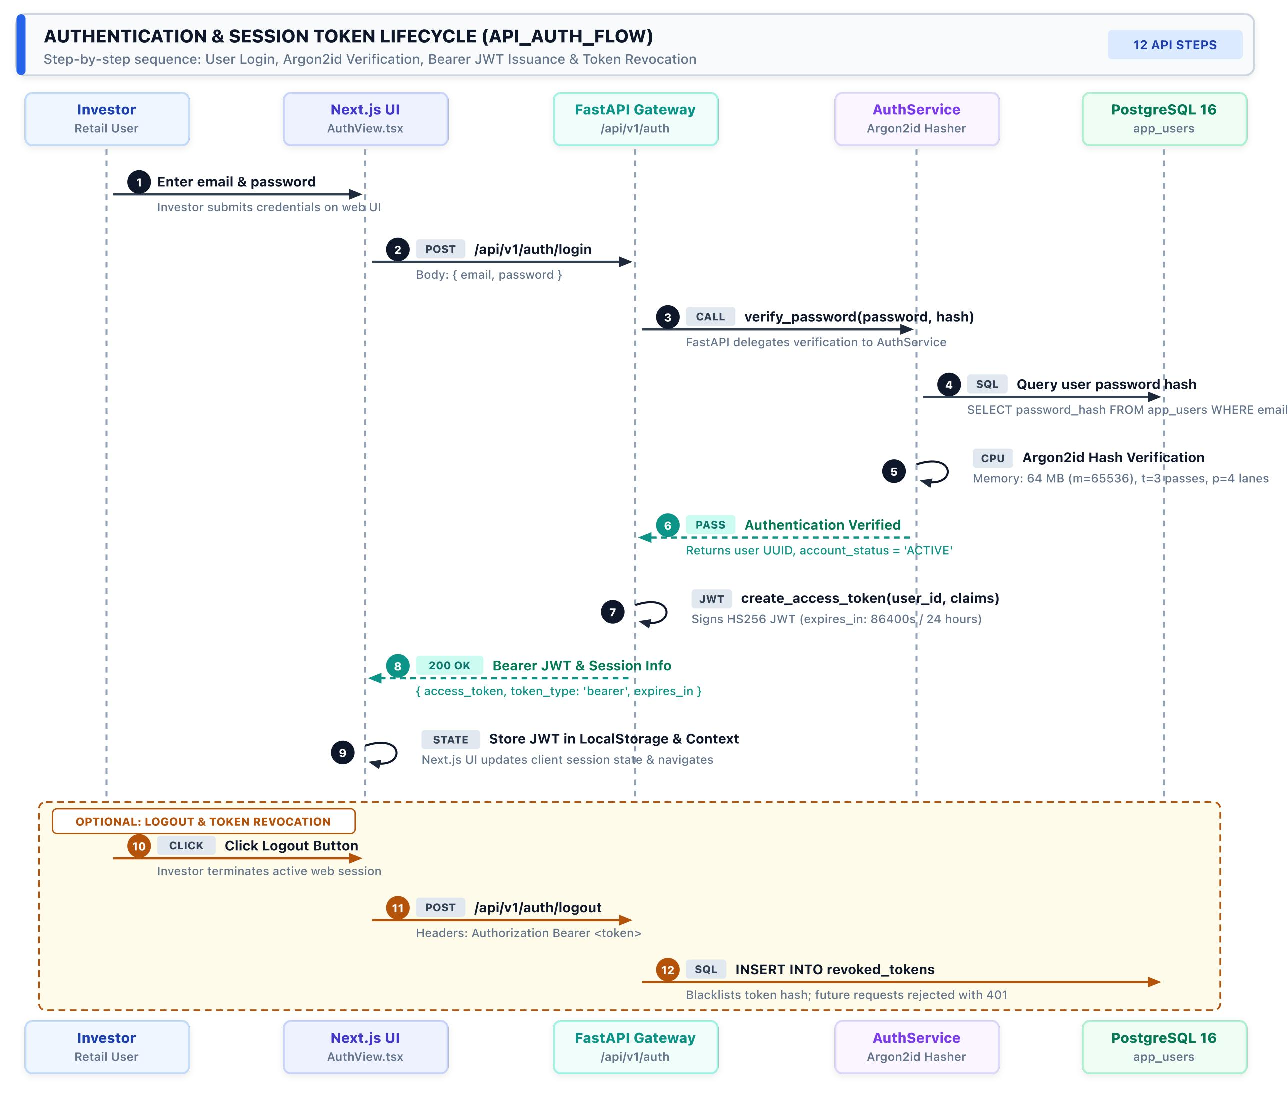
\includegraphics[width=\textwidth, height=0.72\textheight, keepaspectratio]{API_AUTH_FLOW.pdf}
    \caption{API Sequence Diagram: User Registration, Login, and Session Token Flow}
    \label{fig:api_auth_seq}
\end{figure}

\clearpage
\begin{figure}[p]
    \centering
    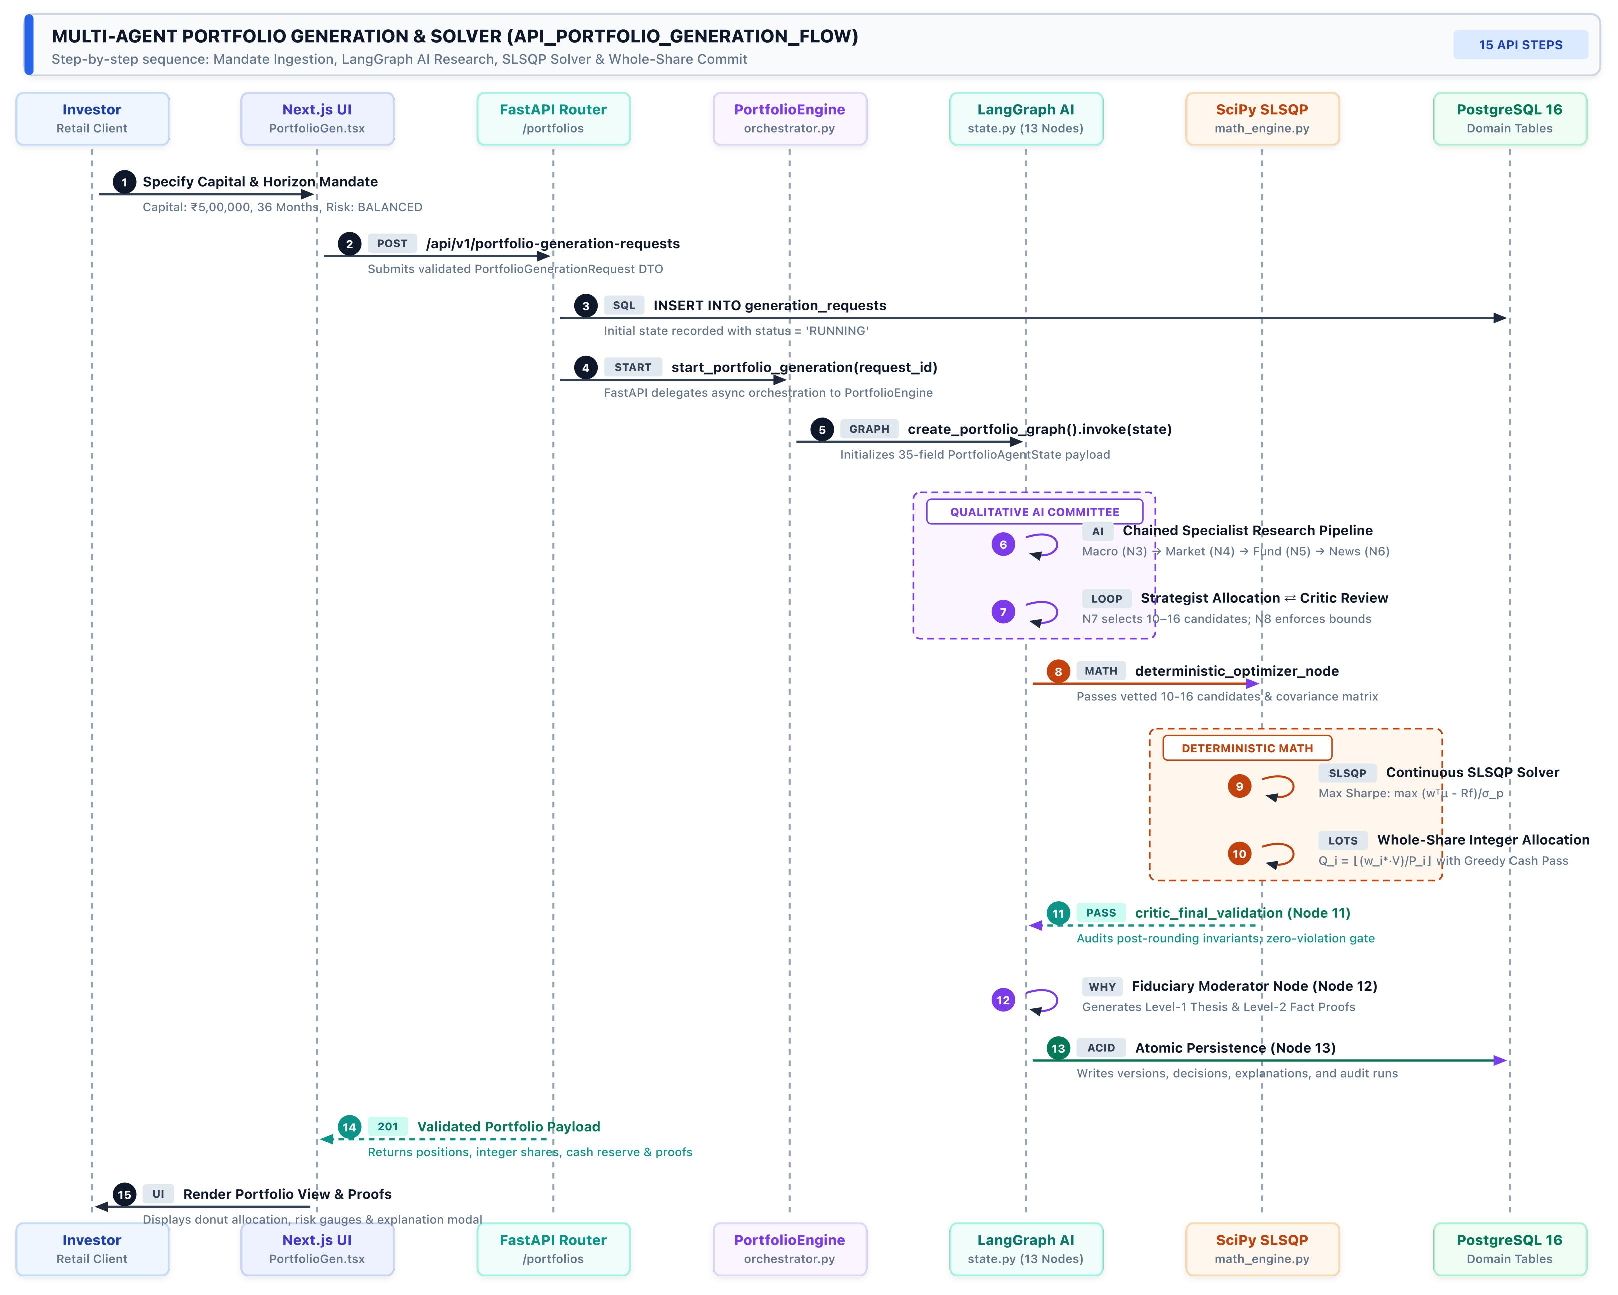
\includegraphics[width=\textwidth, height=0.72\textheight, keepaspectratio]{API_PORTFOLIO_GENERATION_FLOW.pdf}
    \caption[API Sequence Diagram: Multi-Agent Portfolio Solver Flow]{API Sequence Diagram: Multi-Agent Portfolio Generation and Solver Flow}
    \label{fig:api_port_seq}
\end{figure}

\clearpage
\begin{figure}[p]
    \centering
    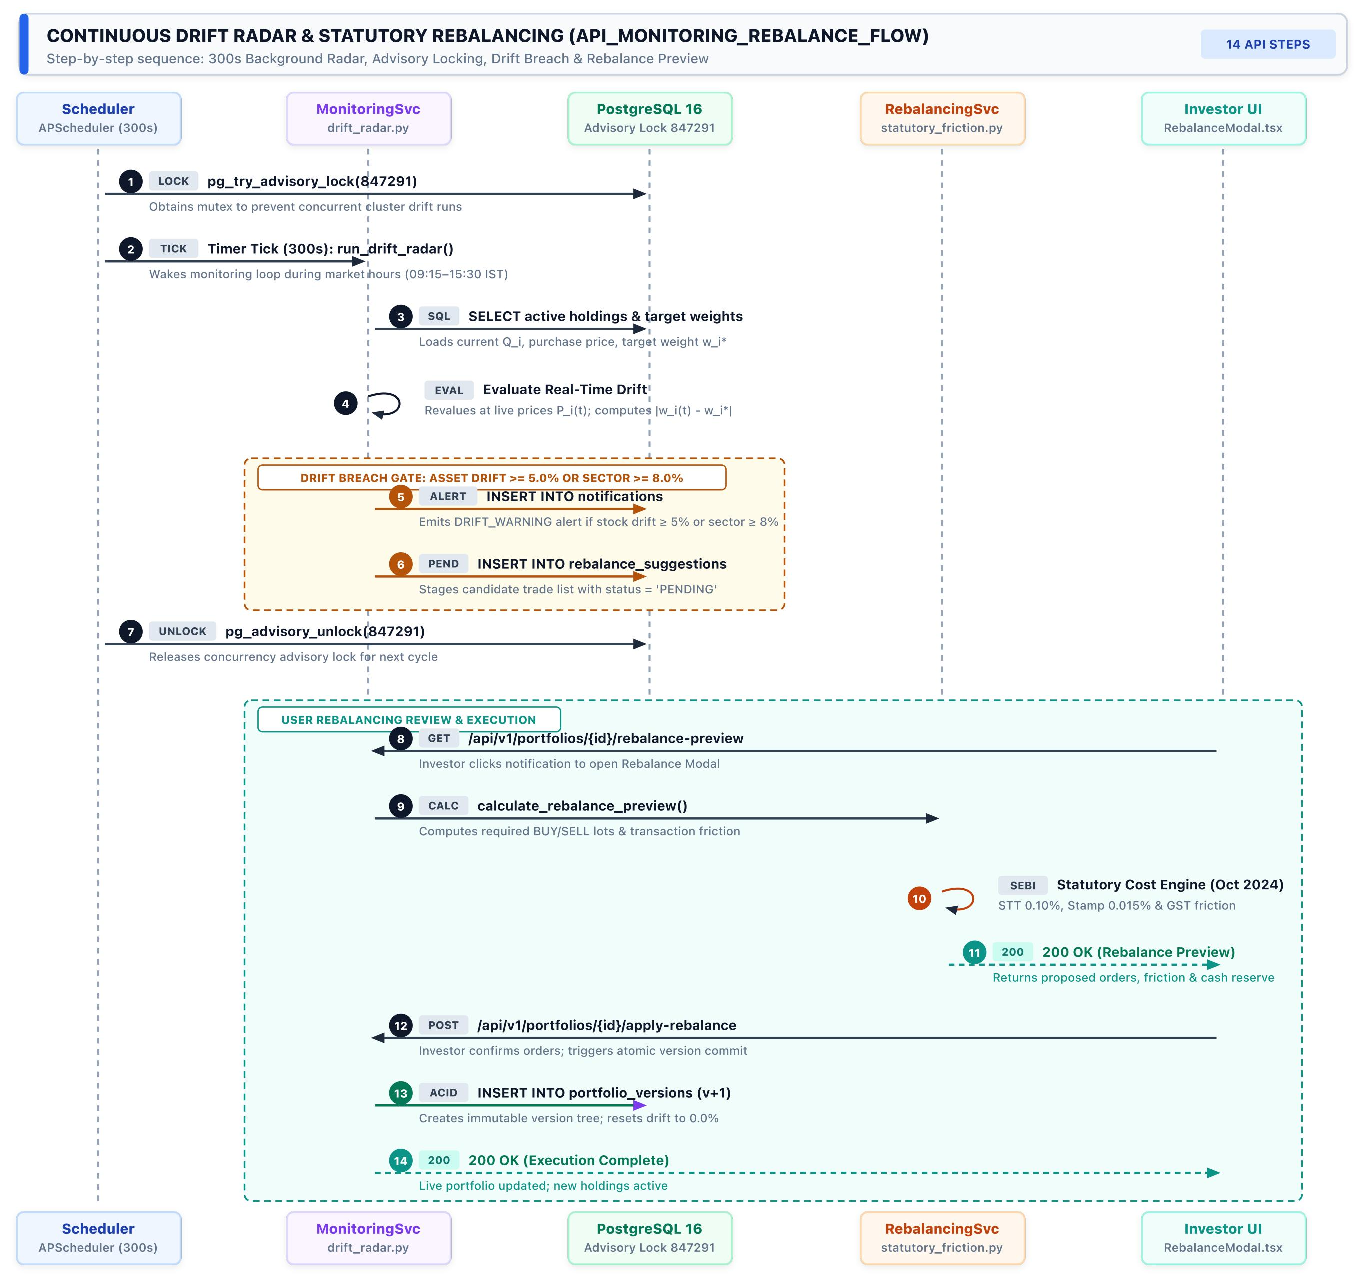
\includegraphics[width=\textwidth, height=0.72\textheight, keepaspectratio]{API_MONITORING_REBALANCE_FLOW.pdf}
    \caption{API Sequence Diagram: Continuous Drift Radar and Rebalance Preview Flow}
    \label{fig:api_mon_seq}
\end{figure}

\clearpage
\begin{figure}[p]
    \centering
    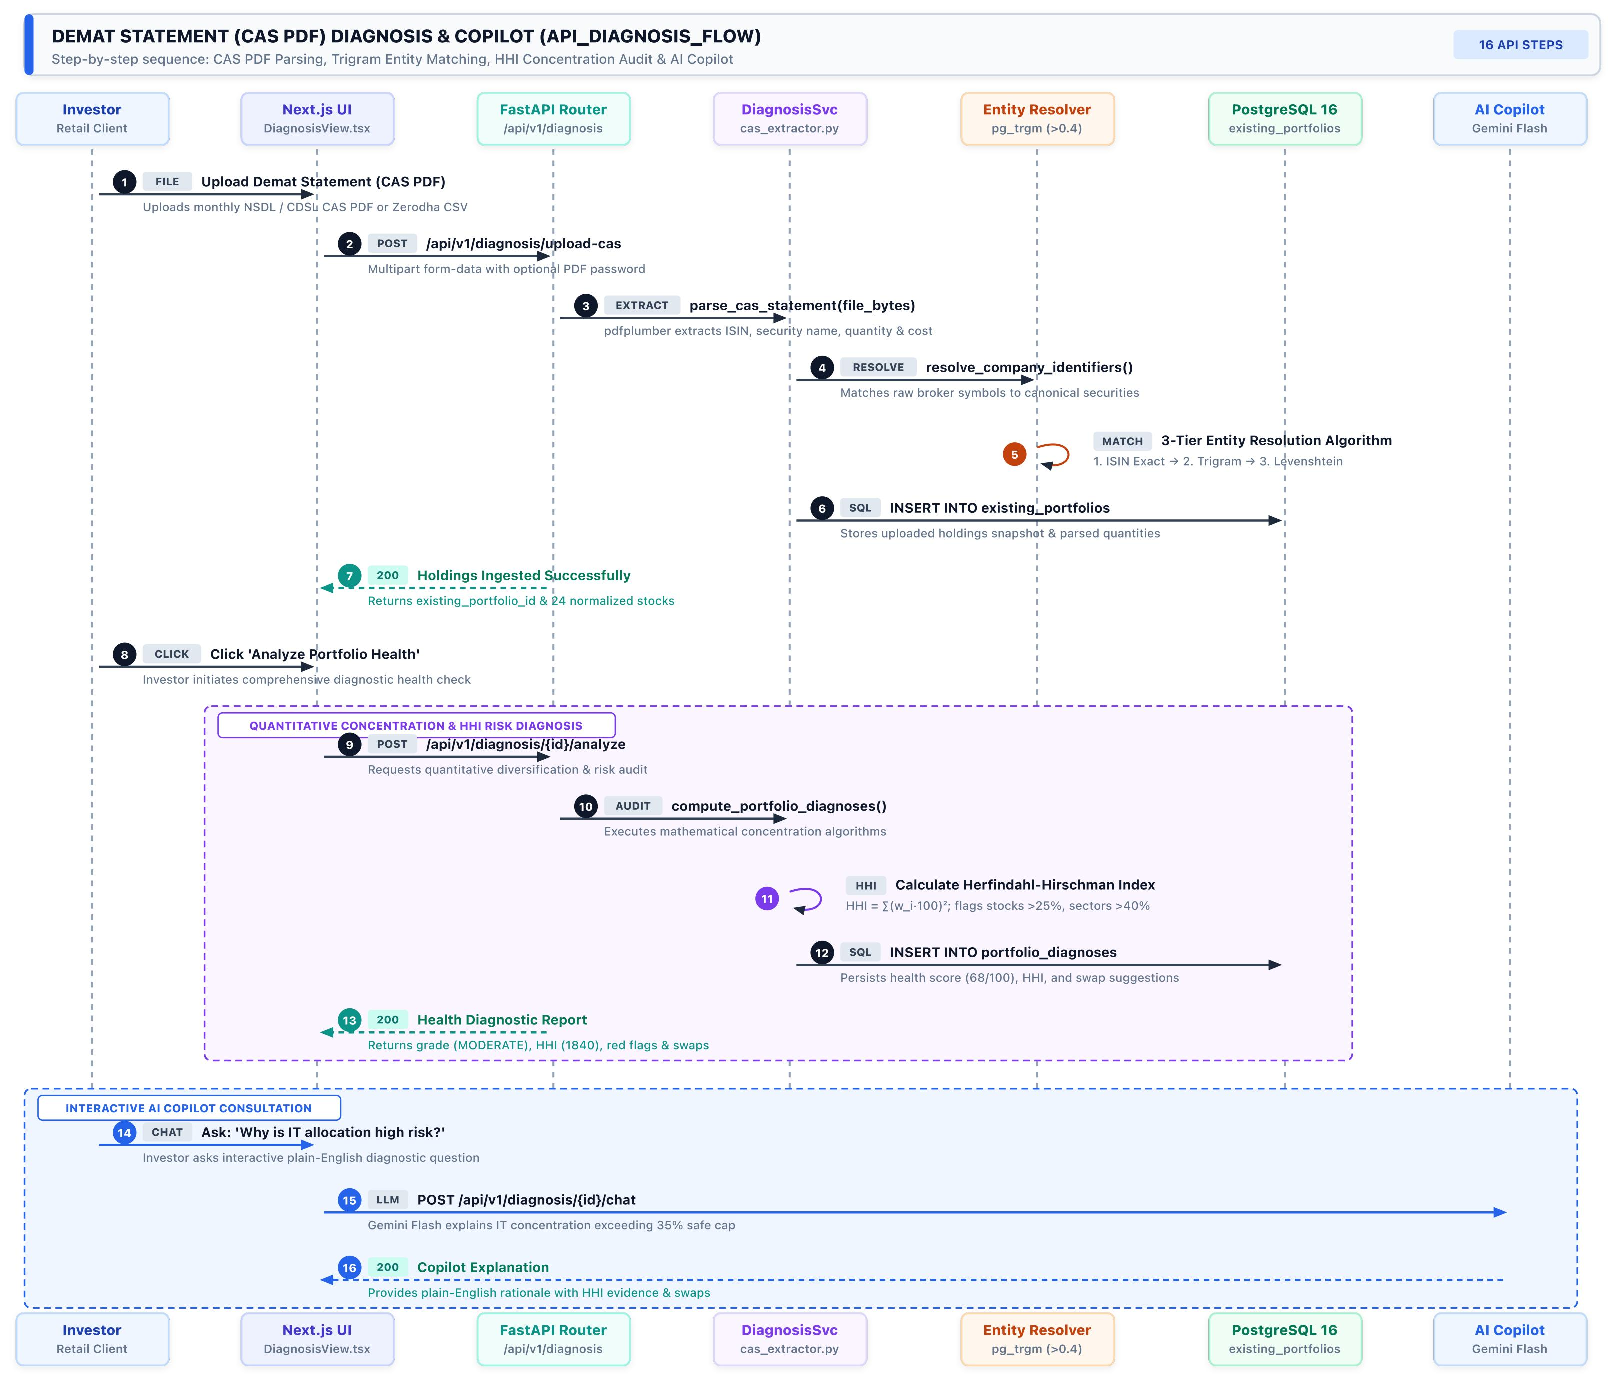
\includegraphics[width=\textwidth, height=0.72\textheight, keepaspectratio]{API_DIAGNOSIS_FLOW.pdf}
    \caption{API Sequence Diagram: Demat CAS Statement PDF Diagnosis Flow}
    \label{fig:api_diag_seq}
\end{figure}
\clearpage

\subsection{Postman Collection and Developer Testing Tools}
To allow engineers and system auditors to test the API easily, Lucid provides an importable Postman collection located in \texttt{postman/}:
\begin{itemize}
    \item \textbf{Collection File (\path{Lucid_API_Collection.json})}: Contains \textbf{96 API requests} organized across 16 folders covering all features.
    \item \textbf{Environment File (\path{Lucid_Development_Environment.json})}: Configured with server URLs and test developer credentials.
    \item \textbf{Automated Test Scripts}: When a developer runs the login request, Postman automatically captures the new session token and saves it into the active environment. All subsequent requests use this token automatically, enabling one-click test runs across the entire platform.
\end{itemize}

